% Use only LaTeX2e, calling the article.cls class and 12-point type.

\documentclass[12pt]{article}
%\usepackage[textwidth=18.5cm]{geometry}
\usepackage[textwidth=18.5cm, textheight=26cm]{geometry}
%\usepackage[a4paper, total={8in, 11in}, margin=1in]{geometry}
% Users of the {thebibliography} environment or BibTeX should use the
% scicite.sty package, downloadable from *Science* at
% http://www.sciencemag.org/authors/preparing-manuscripts-using-latex 
% This package should properly format in-text
% reference calls and reference-list numbers.

\usepackage{adjustbox}
%\usepackage{scicite}

\usepackage{times}
\usepackage{units}

%\usepackage[T1]{fontenc}
%\usepackage[ngerman]{babel}
\usepackage[english]{babel}
\usepackage{empheq}

\usepackage[]{graphicx}
\graphicspath{ {./fig/} }
\usepackage[utf8]{inputenc}
\usepackage{subcaption}
\usepackage[labelformat=simple]{subcaption}  
\captionsetup[subfigure]{font={bf,small}, skip=1pt, margin=-0.1cm, singlelinecheck=false}
\usepackage[labelfont=bf]{caption}
\captionsetup{labelfont=bf}
\captionsetup{font=footnotesize}


\usepackage{amsmath}
\usepackage{booktabs} % Add this to your preamble
\usepackage{adjustbox} % Already used
\usepackage{array} % For better column formatting
\usepackage{amssymb}
\usepackage{cancel}
\usepackage{dirtytalk}
\usepackage{fourier}
\usepackage{siunitx}
\usepackage{tcolorbox}
\usepackage{textgreek}
\usepackage{wrapfig}
\usepackage{tikz}
\newcommand*\circled[1]{\tikz[baseline=(char.base)]{
		\node[shape=circle,draw,inner sep=2pt] (char) {#1};}}

% Added by authors
\usepackage{siunitx}
\usepackage{tabularx,ragged2e,booktabs}
\usepackage{multirow}
\usepackage{lipsum}
\usepackage{bm}
\usepackage{mathtools}
\captionsetup[figure]{name={Fig.},labelsep=period}
%\captionsetup[table]{name={Table},labelsep=period}
\usepackage{hyperref}
\usepackage{xcolor}
\usepackage[normalem]{ulem}
\usepackage{hyperref}
\urlstyle{same}

\usepackage{xr}

\usepackage[nolist]{acronym}
\newacro{ai}[AI]{artificial intelligence}
\newacro{dai}[DAI]{disembodied artificial intelligence}
\newacro{eai}[EAI]{embodied artificial intelligence}

\newacro{gpu}[GPU]{graphics processing unit}
\newacro{cce}[CCE]{computation and communication expenditure}
\newacro{bee}[BEE]{basal energy expenditure}
\newacro{mie}[MIE]{motion and interaction expenditure}


\newacro{isl}[IsL]{isolated learning}
\newacro{il}[IL]{incremental learning}
\newacro{tl}[TL]{transfer learning}
\newacro{til}[TIL]{transfer with incremental learning}
\newacro{cl}[CL]{collective learning}
\newacro{dcl}[DCL]{distributed collective learning}
\newacro{slad}[SLAD]{simultaneous learning and discovery}

\newacro{c1}[C1]{first energy challenge}
\newacro{c2}[C2]{second energy challenge}
\newacro{c3}[C3]{third energy challenge}


\externaldocument{supplementary_materials}


%\usepackage[demo]{graphicx}
%\usepackage{ifdraft}
%\ifdraft{\renewcommand{\includegraphics}{\relax}}{\relax}
%\usepackage{comment}
%\excludecomment{figure}
%\let\endfigure\relax


\newcommand\hl[1]{\colorbox{yellow}{\textcolor{red}{#1}}}
\newcommand\myhl[1]{\textcolor{blue}{#1}}



% Use this to display line numbers
\usepackage{lineno}
\linenumbers

\DeclareMathAlphabet\mathbfcal{OMS}{cmsy}{b}{n}
\DeclareMathAlphabet{\mathcal}{OMS}{cmsy}{m}{n}
\renewcommand{\emph}[1]{\textit{#1}}
\let\textcircledold\textcircled

\renewcommand{\textcircled}[1]{\raisebox{.5pt}{\textcircledold{\raisebox{-.45pt} {#1}}}}
\newcommand*{\important}[1]{\textcolor{red}{\danger~\textbf{IMPORTANT:~}} \textcolor{red}{#1}}
\newcommand*{\pending}[1]{\textcolor{blue}{$\bigstar$~\textbf{PENDING~#1}}}
\newcommand\mybox[2][]{\tikz[overlay]\node[fill=blue!100,inner sep=4pt, anchor=text, rectangle, rounded corners=1mm,#1] {#2};\phantom{#2}}

\newcommand{\TODO}[1]{\mybox[fill=yellow]{\textcolor{blue}{\warning~\Large \textbf{TODO}}:~\textcolor{blue}{\textbf{\emph{#1}}}}}
\newcommand{\xmark}{\ding{55}}%
\newcommand{\textcircledD}[1]{\raisebox{.9pt}{\textcircled{\raisebox{+.5pt} {\footnotesize#1}}}}
\newcommand{\diaz}[1]{\textcolor{blue}{[Diaz: #1]}}
\newcommand{\haddadin}[1]{\textcolor{red}{[Haddadin: #1]}}
\newcommand{\del}[1]{\textcolor{orange}{\xout{#1}}}
\newcommand{\new}[1]{\textcolor{orange}{#1}}
\DeclareMathOperator*{\E}{\mathbb{E}}
\renewcommand{\thesubfigure}{\textbf{\Alph{subfigure}}}
\newtheorem{assumption}{Modeling Assumption}
\newtheorem{definition}{Definition}

\renewcommand{\figurename}{Fig.}


%% MY ADDED SECTION
\usetikzlibrary{backgrounds}
\makeatletter

\tikzset{%
	fancy quotes/.style={
		text width=\fq@width pt,
		align=justify,
		inner sep=1em,
		anchor=north west,
		minimum width=\linewidth,
	},
	fancy quotes width/.initial={.8\linewidth},
	fancy quotes marks/.style={
		scale=8,
		text=white,
		inner sep=0pt,
	},
	fancy quotes opening/.style={
		fancy quotes marks,
	},
	fancy quotes closing/.style={
		fancy quotes marks,
	},
	fancy quotes background/.style={
		show background rectangle,
		inner frame xsep=0pt,
		background rectangle/.style={
			fill=gray!25,
			rounded corners,
		},
	}
}

\newenvironment{fancyquotes}[1][]{%
	\noindent
	\tikzpicture[fancy quotes background]
	\node[fancy quotes opening,anchor=north west] (fq@ul) at (0,0) {``};
	\tikz@scan@one@point\pgfutil@firstofone(fq@ul.east)
	\pgfmathsetmacro{\fq@width}{\linewidth - 2*\pgf@x}
	\node[fancy quotes,#1] (fq@txt) at (fq@ul.north west) \bgroup
}
{\egroup;
	\node[overlay,fancy quotes closing,anchor=east] at (fq@txt.south east) {''};
	\endtikzpicture}

\makeatother
\newcommand{\task}{\ensuremath{\tau}}
\newcommand{\sltwoi}{\ensuremath{t_l}} %single learning time without index
\newcommand{\slt}[1]{\ensuremath{t_{l,#1}}} %... with index
\newcommand{\tlt}{\ensuremath{T}} %total learning time
\newcommand{\comp}{\ensuremath{c}} %complexity (learning time from scratch)
\newcommand{\diste}[1]{\ensuremath{\mathrm{d}(\task_{#1},\{ \})}}
\newcommand{\dist}[2]{\ensuremath{\mathrm{d}(\task_{#1},\{\task_1, \task_2, \dots, \task_{#2}\})}}
\newcommand{\En}{\ensuremath{E}}
\newcommand{\opt}{\ensuremath{\mathrm{opt}}}
\newcommand{\tot}{\ensuremath{\mathrm{tot}}}
\newcommand{\Opt}{\ensuremath{\mathrm{Opt}}}
\newcommand{\densMan}{\ensuremath{\rho_{\mathrm{man}}}} %manufacturing energy density
\newcommand{\Tau}{\ensuremath{\mathcal{T}}}

\newcommand{\redtext}[1]{\textcolor{red}{#1}}
\setlength{\columnsep}{1cm}

\newtheorem{challenge}{\textbf{CHALLENGE}}

\renewcommand{\arraystretch}{2} 

% The preamble here sets up a lot of new/revised commands and
% environments.  It's annoying, but please do *not* try to strip these
% out into a separate .sty file (which could lead to the loss of some
% information when we convert the file to other formats).  Instead, keep
% them in the preamble of your main LaTeX source file.


% The following parameters seem to provide a reasonable page setup.
\topmargin 0.0cm
\oddsidemargin 0.2cm
\textwidth 16cm 
\textheight 21cm
\footskip 1.0cm


%The next command sets up an environment for the abstract to your paper.
\newenvironment{sciabstract}{%
\begin{quote} \bf}
{\end{quote}}


% Include your paper's title here
% \title{\textbf{Title:} From Many, One Mind: Collective Learning for Sustainable AI and Robotics}

% \title{\textbf{Title:} All for One and One for All: The Sustainable Knowledge Composition Dynamics for Collective EAI}

\title{Collective Simultaneous Learning and Discovery of Knowledge for Scalable Yet Sustainable Embodied AI}


% Place the author information here.  Please hand-code the\\
% information and notecalls; do *not* use \footnote commands.  Let the
% author contact information appear immediately below the author names
% as shown.  We would also prefer that you don't change the type-size
% settings shown here.

\author
{Fernando D\'iaz Ledezma$ {}^{1}$ and Sami Haddadin${}^{2,\ast}$
	\\
	%\normalsize{\textbf{Affiliations:} \normalsize{${}^{1}$TUM - Technical University of Munich}}\\
	\normalsize{${}^{2}$MBZUAI - Mohamed bin Zayed University of Artificial Intelligence}\\
	\\
	\normalsize{$^\ast$To whom correspondence should be addressed; E-mail: \url{sami.haddadin@mbzuai.ac.ae}}
}
% Include the date command, but leave its argument blank.

\date{}



%%%%%%%%%%%%%%%%% END OF PREAMBLE %%%%%%%%%%%%%%%%



\begin{document} 
% Double-space the manuscript.

\baselineskip24pt

% Make the title.

\maketitle 



% Place your abstract within the special {sciabstract} environment.
\begin{sciabstract}
	\textbf{Abstract:}
    % The current learning paradigms in \ac{dai} are characterized by substantial energy consumption, primarily due to intensive computational processes and limited utilization of acquired knowledge. As \ac{ai} converges with robotics to form \ac{eai} systems, their energy demands are poised to escalate further because data acquisition and learning necessitate continuous interaction with the physical environment. This study delves into the core energy requirements of \ac{eai} systems and explores the energy-related challenges linked to maintaining existing learning paradigms. Consequently, we advocate for collective learning, a paradigm shift that promotes efficient learning in \ac{eai} agents by actively sharing, aggregating, and leveraging past and current knowledge across systems. This approach is pivotal for reducing energy consumption and expediting the acquisition of new skills.
As \ac{ai} becomes increasingly embodied in physical agents---robots, vehicles, drones---the energy demands of learning and adaptation rise sharply. Unlike disembodied \ac{ai}, which relies on computational training detached from physical action, \ac{eai} systems must interact continuously with the real world, incurring motion, interaction, and communication energy costs. In this work, we analyze the fundamental energy expenditures of \ac{eai} and identify the limitations of conventional learning paradigms---isolated, incremental, and transfer learning---in large-scale robotic deployments. We propose \ac{cl} as a scalable, energy-efficient alternative that leverages structured inter-agent knowledge sharing. We present a dynamical systems model of CL on a structured skill manifold and reveal nine canonical regimes of learning behavior, determined by intra-agent memory retention and inter-agent knowledge sharing. Our results demonstrate that CL dramatically reduces learning episodes and energy consumption---by a substantial margin compared to the closest conventional alternative---especially as the number of agents increases. Through simulation and a smart factory case study, we show that CL achieves superior skill acquisition while enabling zero-shot learning and minimal production downtime. These findings position \ac{cl} as a key enabler for sustainable, scalable, and adaptive \ac{ai} in robotics and beyond.    
\end{sciabstract}

%\textbf{One-Sentence Summary:} Embracing collective learning in (embodied) AI reduces energy consumption and accelerates skill acquisition by orders of magnitude.

% In setting up this template for *Science* papers, we've used both
% the \section* command and the \paragraph* command for topical
% divisions.  Which you use will of course depend on the type of paper
% you're writing.  Review Articles tend to have displayed headings, for
% which \section* is more appropriate; Research Articles, when they have
% formal topical divisions at all, tend to signal them with bold text
% that runs into the paragraph, for which \paragraph* is the right
% choice.  Either way, use the asterisk (*) modifier, as shown, to
% suppress numbering.

%%%%%% Main Text %%%%%%

\newcommand{\beginsupplement}
{%
	\setcounter{table}{0}
	\renewcommand{\thesection}{S\arabic{section}}
	\renewcommand{\thetable}{S\arabic{table}}%
	\setcounter{figure}{0}
	\renewcommand{\thefigure}{S\arabic{figure}}%
}

% ===================================================================================================
%                                                 |                                                 |
%                                                 |                                                 |
% -------------------------------------------- SECTION ---------------------------------------------|
%                                                 |                                                 |
%                                                 |                                                 |
% ===================================================================================================
\section*{Main Text:}

\Ac{ai}-powered technology, especially machine learning, is increasingly integrated into daily life. We anticipate a future with smart factories, \ac{ai}-enhanced healthcare services, and automated homes. Modern robots, equipped with advanced computing and communication capabilities, will become ubiquitous in industry, logistics, service, and healthcare. These robots will take advantage of \ac{ai} to acquire new skills and share knowledge between systems, integrate synergistically with various environments, and collaborate with humans on various tasks. However, this growing ubiquity of \ac{ai} and robotics also presents significant challenges, particularly with regard to their energy demands.

% ===================================================================================================
\paragraph*{The grand energy challenges in \ac{ai}}
Rapid advancements driven by \ac{ai} applications come at a substantial energy cost. This constitutes the \underline{\ac{c1}}. Cutting-edge machine learning algorithms require immense computational power to process, analyze, and learn from vast datasets, often requiring numerous iterations to converge \cite{Strubell2019EnergyPolicyConsiderations}. Researchers and companies rely heavily on available on-premise infrastructure or cloud computing services in data centers for these energy-intensive workloads during the learning and deployment phases. This has led to a clear spike in energy consumption in an ever-increasing number of data centers and associated hardware such as GPUs. Training \ac{ai} models in data centers is estimated to consume about three times more energy than traditional cloud tasks, significantly straining resources \cite{Thomas2023cloudusesmassive}.

Consider the latest breakthroughs in generative \ac{ai}, including large language models (LLMs), text-to-image, and text-to-video models. These models, with billions of parameters, require thousands of deep learning GPU units and millions of GPU hours for training \cite{Vanian2023ChatGPTgenerativeAI, Corbyn2023Nvidiachipmaker}. As more \ac{ai} applications are developed, the demand for \ac{ai} infrastructure surges, leading to a substantial increase in GPU-based \ac{ai} server sales. This escalation directly translates into a parallel increase in data center energy consumption. Globally, data center energy consumption rose from 200 TWh in 2015 to an estimated 220-320 TWh in 2021, according to the International Energy Agency\footnote{Data from the International Energy Agency, available at \url{https://www.iea.org/reports/data-centres-and-data-transmission-networks}}. This concerning trend is illustrated in Fig.~\ref{fig:energy_consumption_trends_ai_and_robotics}~(\textbf{A})).

The \underline{\ac{c2}}, the escalating energy demand of a potential robotic revolution, is amplified by the rise of Industry 4.0, the implementation of smart factories, and the expanding use of robots in service applications. This rapid proliferation has even been dubbed the ``Cambrian explosion'' of robotics \cite{Pratt2015Iscambrianexplosion}. Despite advances in robot technology that have improved energy efficiency, the focus remains predominantly on individual systems, often overlooking the aggregate impact of all active units.

During the past decade, the installed base of industrial robots has undergone a remarkable transformation. According to the International Federation of Robotics (IFR), this base grew from 1.2 million units in 2012 to approximately 4.2 million units in 2023, an astonishing increase of 350~\% with an average annual growth rate close to 12~\% \cite{IFR2024WorldRobotics2024}. Extrapolating this trend suggests that within the coming years, six million robots will be operational in factories worldwide\footnote{These projections closely align with the slightly more cautious estimates presented by *The Boston Consulting Group* in \cite{Sirkin2015HowRobotsWill}.}. Using this estimated installed base and assuming round-the-clock operation, we can approximate the forthcoming energy demand attributable to industrial robots, termed the World Robot Energy Consumption (WREC), as shown in Fig.~\ref{fig:energy_consumption_trends_ai_and_robotics} (\textbf{B}). To contextualize the significance of WREC, in 2025, it is projected to constitute 7.2~\% of Germany's installed power generation capacity \cite{FraunhoferISENetinstalledelectricity}, one of the most industrialized countries in the world. A detailed description of these estimates is provided in Sec.~\ref{sec:app_robot_ener_consumption}.

The far-reaching influence of collaborative and even service robots mirrors the significance observed among their industrial counterparts. Collaborative robots (cobots), for instance, have undergone a paradigm shift, rising from a mere 6~\% of the market in 2017 to accounting for approximately one-quarter of annual installations \cite{tobe2015}, as illustrated in Fig.~\ref{fig:industrial_cobot_share}. Drawing from analogous assumptions applied to industrial robots, Fig.~\ref{fig:energy_consumption_trends_ai_and_robotics} (\textbf{C}) depicts the projected growth trajectory of cobots and their associated energy consumption. Concurrently, the domain of service robots is experiencing an analogous surge. For example, estimates projected that the service robotics market would reach 56 billion euros by 2025 \cite{statista_service_robots}. These robots are used in various fields, including logistics, defense, public relations, and medical applications, aligning with the increasing trends observed among industrial and collaborative robots.

The \underline{\ac{c3}}, often overlooked in the realm of \ac{ai}, is the energetic expenditure associated with the actual manufacture of the hardware required for \ac{ai} and robotics. This energy demand encompasses two primary facets. First, it involves the energy expenditure to procure materials for robot manufacturing and associated computational hardware (for example, processors, GPUs, and \ac{ai} servers). Second, it pertains to the intrinsic energy consumption of the manufacturing process itself. Given the direct correlation between energy demand and the number of \ac{ai}-powered robots produced, an exponential increase in the latter directly corresponds to the increase in the energy consumption for their production. Assessment and formulation of strategies to address this aspect are crucial. Although an immediate solution may not be evident and substantial energy savings in the procurement of raw materials may be impractical, significant potential lies in the recycling of electronic components of computer and robot hardware as a means of conserving energy \cite{Ude2025Recycling}.

% \footnote{An example of such an endeavor is the international competition Robothon\textsuperscript{\textregistered} - The Grand Challenge, see \url{[https://automatica-munich.com/en/munich-i/robothon/](https://automatica-munich.com/en/munich-i/robothon/)}.}.

% ---
\begin{figure*}[t!]
	\centering
	\hspace*{\fill}
	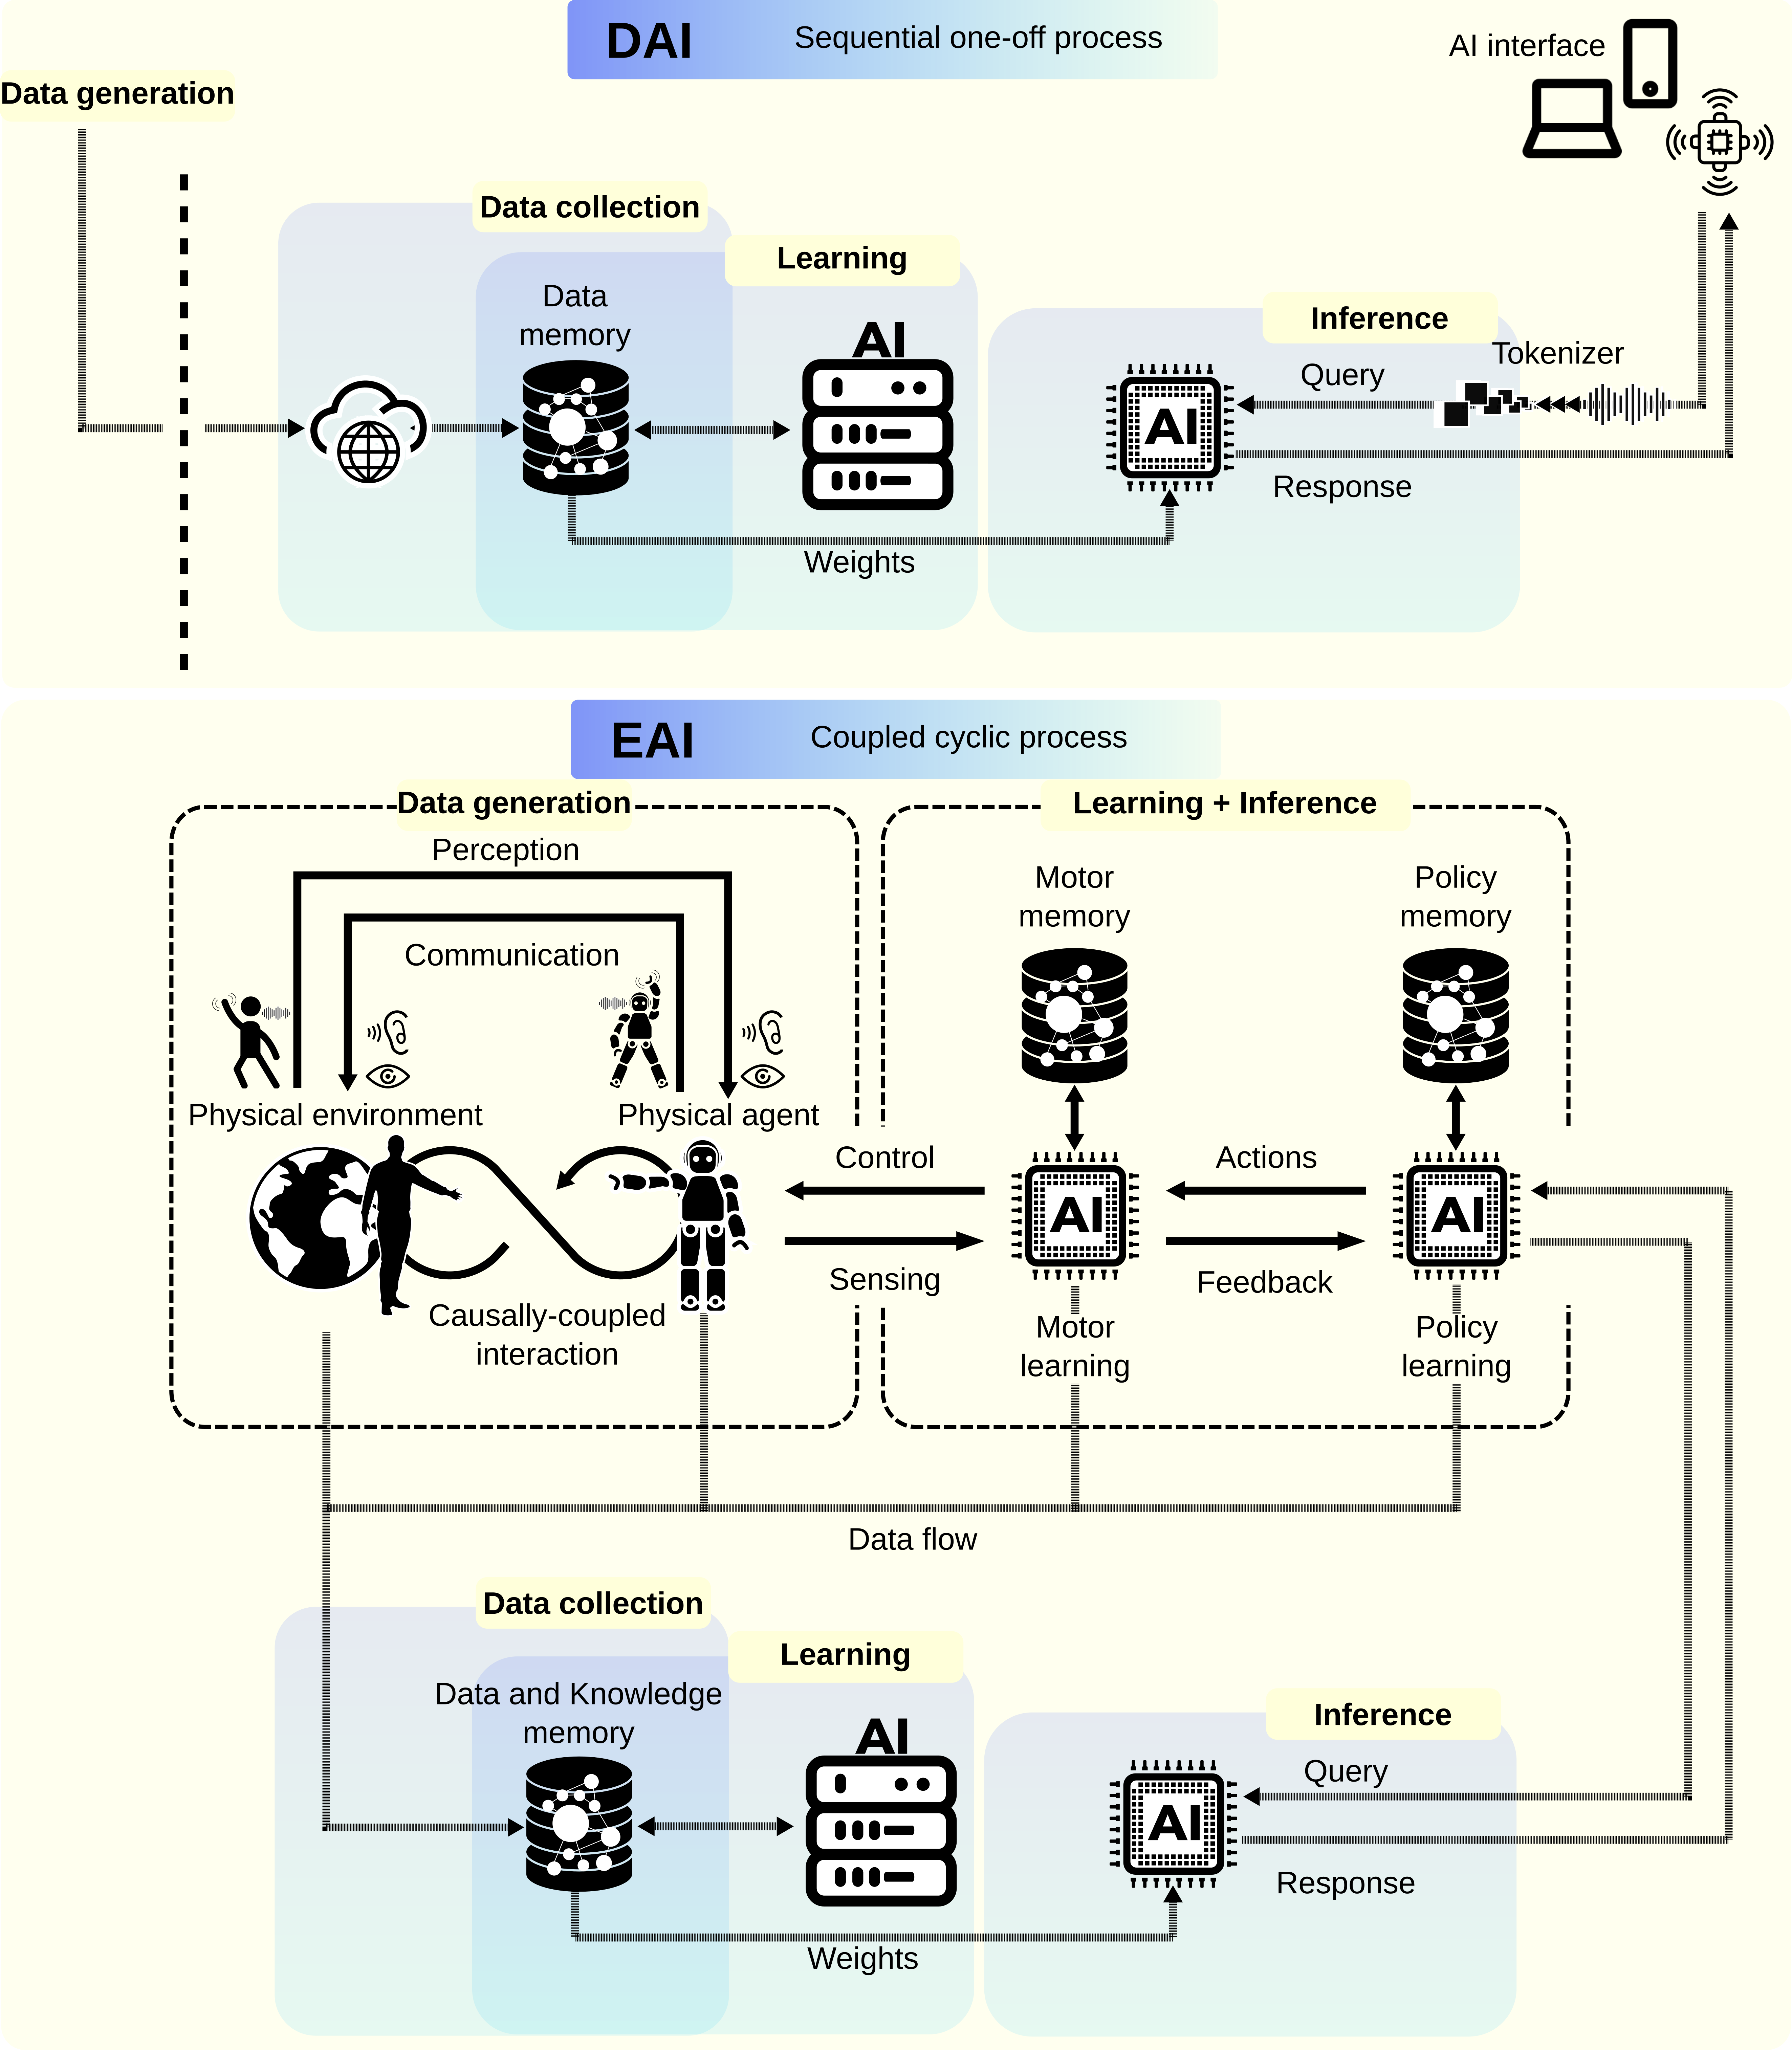
\includegraphics[width=0.95\textwidth]{eai_and_dai_concept_figure.png}
	\hspace*{\fill}
	\caption[] {\label{fig:eai_and_dai_concept_figure} \textbf{Disembodied and embodied \ac{ai}.} (\textbf{A}) In \ac{dai} learning is a sequential one-off process from which data generation is detached. (\textbf{B}) Causally-coupled cyclic interaction of \ac{eai} agents with the environment continuously generating non-repetitive data for learning.}
	
\end{figure*}
% ---

% ===================================================================================================
\paragraph*{Energy Expenditure in Disembodied and Embodied \ac{ai}.} To effectively address the energy demands of \ac{ai} and robotics, we differentiate between classical \acl{dai} and \acl{eai}, as illustrated in Fig.~\ref{fig:eai_and_dai_concept_figure}.

We define \ac{dai} as methods and algorithms that tackle purely computational problems, detached from embodied systems and lacking interaction with our vast physical world (see Fig.~\ref{fig:eai_and_dai_concept_figure}~\textbf{A}). In \ac{dai}, data collection occurs passively through various edge devices, with a prototypical \ac{dai} agent not directly involved in the generation or collection of training data. The energetic demands of \ac{dai} applications primarily stem from learning (training models) and deployment (running inference and prediction) \cite{Vries2023growingenergyfootprint}.

In \ac{dai} applications aimed at various tasks or systems, effective knowledge transfer depends on whether the learning approach is suitable and whether the model and training data adequately encapsulate the relevant information for the problem. However, when any of these elements are lacking, it may be essential to retrain, possibly even starting anew, resulting in energy-intensive learning procedures. Even if learning occurs only once, the ongoing deployment of the model can require significant energy due to the constant execution that is computationally intensive \cite{Vries2023growingenergyfootprint}. Thus, depending on the application, the energetic cost of learning and deployment in \ac{dai} can outweigh the benefits \cite{Strubell2019EnergyPolicyConsiderations}. This also applies to recent breakthroughs, such as transformer models for Natural Language Processing, whose results are accompanied by energetic challenges \cite{Cao2020TowardsAccurateReliable}.

The evolution toward \ac{eai}, the integration of \ac{ai} and robotics \cite{Pfeifer2004Embodiedartificialintelligence}, further expands the spectrum of energy use. Unlike virtual environments, the real world cannot be faithfully replicated, despite considerable advances in sim-to-real applications \cite{Chebotar2019Closingsimreal}. Learning and deployment in \ac{eai} demand constant, energy-expending interaction with the physical environment for active data generation, as depicted in Fig.~\ref{fig:eai_and_dai_concept_figure}~\textbf{B}, facilitated by physical agents such as robots, vehicles, and drones. Mastering skills in the physical realm requires continuous and repeated execution, consuming energy for motion and interaction in each instance. Take, for example, autonomous driving, where vehicles function as rudimentary \ac{eai} agents in structured human-made environments. In addition to energy for autonomous movement, vehicles expend additional energy on motion to collect data necessary to retrain and improve the policy model. Another example is the usage of robots to automate a high percentage of chores in essentially limitless variations of household environments~\cite{Lehdonvirta2022futuresunpaidwork}. Such robots will undergo constant retraining due to the subtle and changing dynamics of household environments. Consequently, the case of several \ac{eai} agents learning diverse skills in realistic environments around-the-clock directly influences the potential energy consumption of the skill acquisition process (an example of such a case is discussed in \cite{Johannsmeier2025APM}).

% ---
\begin{figure*}[t!]
	\centering
	\hspace*{\fill}
	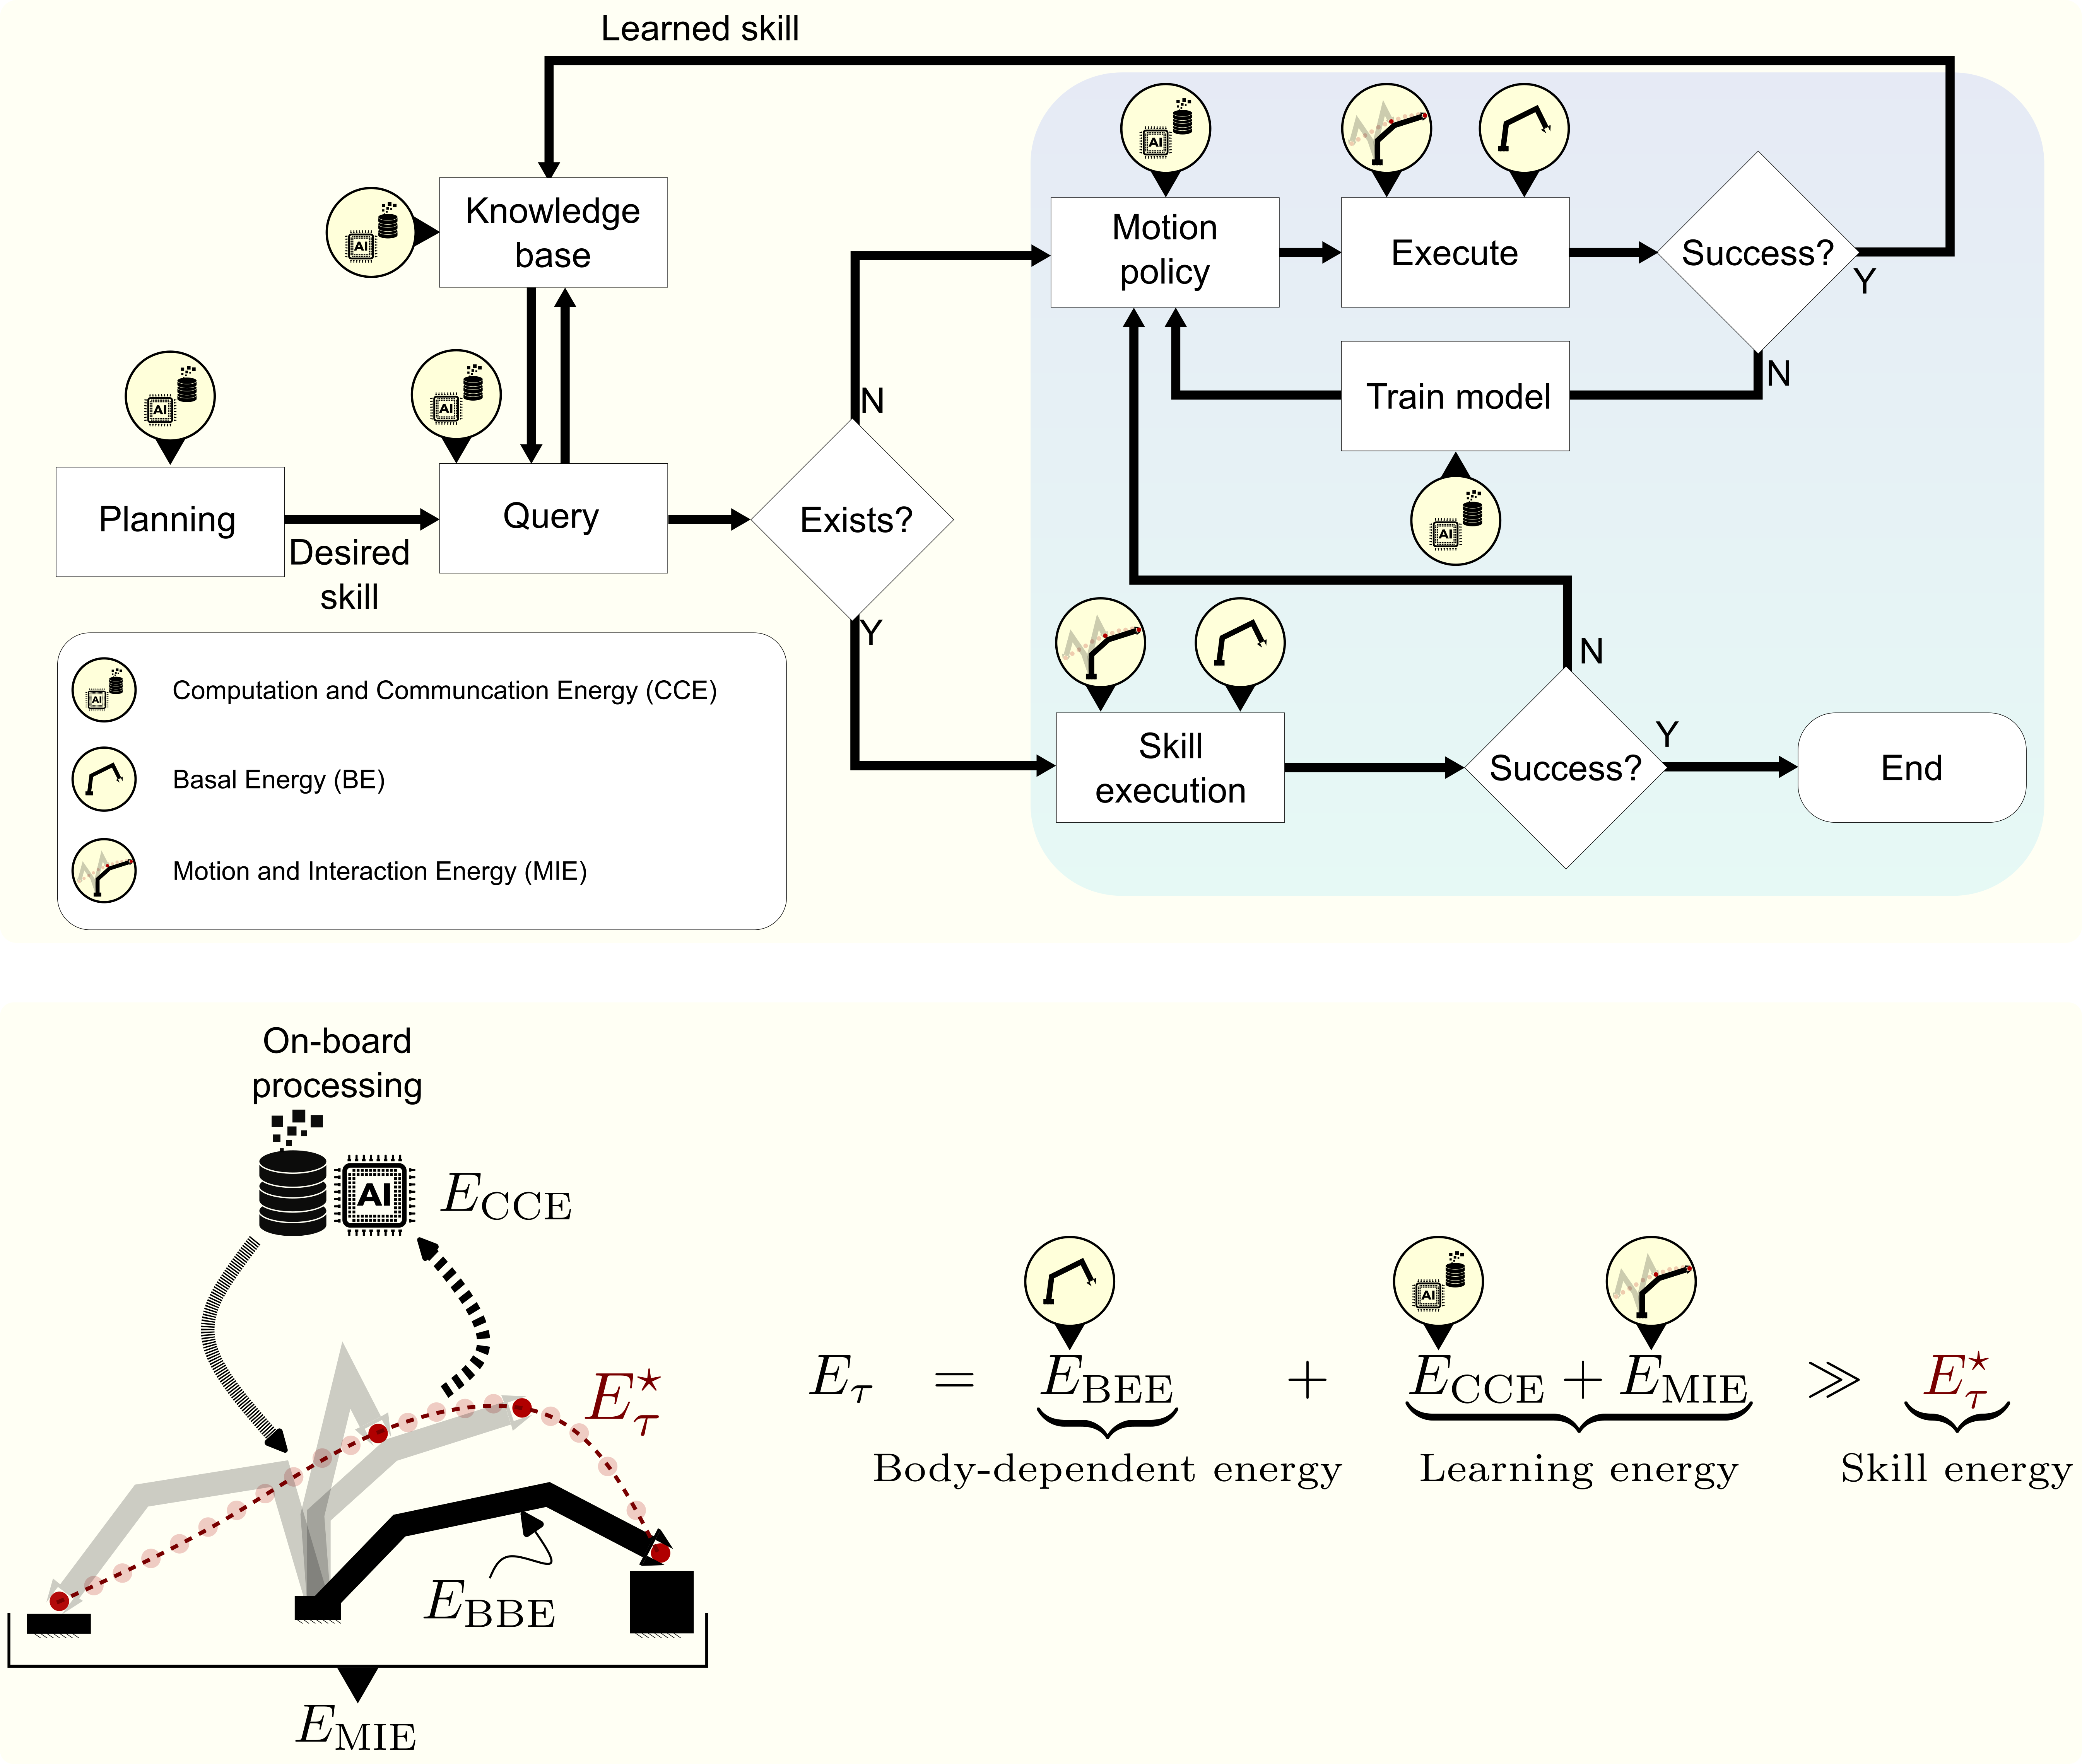
\includegraphics[width=0.95\textwidth]{eai_energy_categories.png}
	\hspace*{\fill}
	\caption[] {\label{fig:embodied_ai_pipeline} \textbf{Energy expenditures of an \ac{eai} agent.} {(\textbf{A}) Standard skill execution pipeline of a prototypical \ac{eai} agent. (\textbf{B}) Three fundamental energy expenditure categories are identified during the planning, learning, and execution of a skill by an \ac{eai} agent.}}
\end{figure*}
% ---

Unlike the standard energy classification for learning and deployment in \ac{dai}, analyzing the energetic requirements in \ac{eai} requires a different perspective. A closer look at the standard skill execution pipeline of a prototypical \ac{eai} agent (Fig.~\ref{fig:embodied_ai_pipeline}) allows for the identification of essential energetic expenditure categories:
% ---
\begin{enumerate}
	\item \Ac{cce}: Coincident with \ac{dai}, this refers to the energy used by computational and communication processes required for planning, querying, exploration, and training routines.
	\item \Ac{bee}: This body-related energy is associated with the execution of basic functions of the \ac{eai} agent. Examples include operating energy, gravity compensation, and proprioceptive intelligence algorithms in robots, hovering in drones, and running on-board system standby in autonomous vehicles.
	\item \Ac{mie}: This defines the energy expended on physical interactions, specifically in executing a particular skill. For instance, moving an object from an initial location to a target location within a given time, following a particular trajectory.
\end{enumerate}
% ---

An important fact in \ac{eai} is the existence of a lower bound on the energy required to perform a skill that is independent of the agent. Consider a generic skill $\tau$---such as a pick-and-place operation---and suppose that the optimal trajectory $p^\star$ for moving an object from its origin to its destination is known. The intrinsic properties of the object and the optimal trajectory $p^\star$ uniquely define the minimum energy requirement $E^\star_{\tau}$ needed to perform the skill $\tau$. The implication is that the total energy expended by any agent in the process of mastering or executing a skill is higher than $E^\star_{\tau}$ as a result of the required energy expenditures for computational ($E_\text{CCE}$), body-related ($E_\text{BEE}$), and physical interaction ($E_\text{MIE}$) energy expenditures; i.e.,
% ---
\begin{equation}\label{eq:skill_energy_in_eai}
	E_{\tau} =  \underbrace{E_\text{BEE}}_{\text{Body-dependent energy}} + \underbrace{E_\text{CCE} + E_\text{MIE}}_{\text{Learning energy}} \gg \underbrace{E^\star_{\tau}}_{\text{Skill energy}} .
\end{equation}
% ---
It is worth mentioning that if Eq.~\eqref{eq:skill_energy_in_eai} were used to describe the energy consumption of a task in \ac{dai}, $E_\text{BEE}$ could be associated with the edge devices, and $E_\text{CCE}$ would represent the primary source of energy consumption. Furthermore, the expenditures $E^\star_{\tau}$ and $E_\text{MIE}$ do not exist in \ac{dai} since physical interaction is absent.



% \paragraph*{Data, information, and knowledge} 
% \myhl{Data, information, and knowledge play distinct roles in embodied learning. Data are raw trial episodes generated through interaction, while information arises when patterns, such as similarities between skills, are extracted to reduce uncertainty. Knowledge is the structured and persistent competence an agent retains, which we formalize as the remaining knowledge function, indicating how much of a given skill remains to be acquired.
% \newline
% Knowledge creation can then be understood in three modes. Accumulation corresponds to storing more skills in memory, with learning rates depending on the number of mastered intra-cluster skills. Integration emerges when intra-cluster similarity, quantified by the retention gain, accelerates acquisition through reuse of related skills. Composition goes further by combining subskills into composite tasks, generating emergent competence that exceeds simple addition. These distinctions frame learning as more than just processing data: it is the creation of knowledge through accumulation, integration, and composition.}


% ===================================================================================================
% \paragraph*{Related Works} The growing trends depicted in Fig.~\ref{fig:energy_consumption_trends_ai_and_robotics} suggest that energy expenditures for computation and communication, basal functions, and motion and interaction will likely follow a similar pattern. The implication is straightforward: as the number of \ac{ai} applications and robotic systems increases, so does their associated energy demand. Consequently, the energy requirements of \ac{dai} and \ac{eai} have recently received significant attention within the \ac{ai} and robotics research communities.
\paragraph*{Related Works} The growing trends depicted in Fig.~\ref{fig:energy_consumption_trends_ai_and_robotics} suggest that energy expenditures for computation and communication, basal functions, and motion and interaction will likely follow a similar pattern. The implication is straightforward: the---arguably exponential---increase in the number of \ac{ai} applications and robotic systems brings with it an increase in their associated energy demand. Consequently, the energy requirements of \ac{dai} and \ac{eai} have recently received significant attention within the \ac{ai} and robotics research communities.

The increasing energy consumption of \ac{ai}, particularly machine learning, has raised concerns about its adverse environmental impact. Most research in this area focuses on the computational and infrastructural requirements for training and running modern learning algorithms---such analyses directly correlate with computational and communication energy expenditure. Recent work has delved into the efficiency of computationally intensive deep learning algorithms \cite{Schwartz2019GreenAI,Vinuesa2020roleartificialintelligence,Strubell2019EnergyPolicyConsiderations,Luccioni2023EstimatingCarbonFootprint}. In parallel, various metrics have been established to gauge the energy consumption of machine learning algorithms. These include evaluating energy efficiency during the development phases \cite{Zhou2020HULKEnergyEfficiency}, analyzing accuracy, model size, time, and CPU/GPU energy consumption for training and inference phases \cite{Dalgren2019GreenMLmethodology}, as well as encompassing other system-level performance indicators such as real-time metrics, instruction-level analysis, and hardware-level power estimation \cite{GarciaMartin2019Estimationenergyconsumption}. Recent work on large language models has discussed various aspects such as hardware efficiency, model architectures, and algorithms in relation to energy consumption \cite{Vries2023growingenergyfootprint} and provides comparisons including their power consumption and CO$_2$ emissions \cite{SIHCAI2023ArtificialIntelligenceIndex}.

Despite growing awareness of \ac{ai}'s energy consumption, tangible actions to address the underlying issues and propose remedies remain scarce and predominantly focus on \ac{dai} applications. However, it is crucial to recognize the challenges posed by \ac{eai} systems. Unlike state-of-the-art machine learning models (for example, transformer models) that are mostly trained once on a large amount of data, \ac{eai} agents have a constant need for energy-consuming retraining and evaluation processes. From the \ac{eai} perspective, ongoing efforts to minimize \ac{bee} and improve \ac{mie} advocate strategies such as elastic energy-aware actuation and optimized hardware selection and storage, energy sharing, and motion planning \cite{CUT2015Smoothrobotmovements, Mohammed2014MinimizingEnergyConsumption, Chemnitz2011Analyzingenergyconsumption,Vasarhelyi2023OverviewEnergiesProblems,Sekala2024SelectedIssuesMethods}.

For \ac{cce}, it is essential to design better hardware for more efficient parallel computing and to decentralize computation, using the local processing capabilities of edge devices and robots. These capabilities have been highlighted in concepts such as the Internet of Robotic Things \cite{Vermesan2020InternetRoboticThings,Sekala2024SelectedIssuesMethods}. Perhaps even more relevant is to define sample-efficient algorithms with optimized models that account for the recurrent learning, inference, and prediction processes in \ac{eai} agents. We believe that achieving greater energy efficiency in \ac{ai} requires a broader perspective than just improving hardware and optimizing individual agents' learning strategies. The actual key to a significant breakthrough lies in tapping into the vast reservoir of knowledge accumulated by \ac{eai} systems.

% ===================================================================================================
\paragraph*{\Acl{cl} for \ac{eai}} The rapid proliferation of robotic agents and advances in \ac{ai} present a pressing challenge: the rising energy demands of contemporary learning paradigms. These paradigms---primarily designed for disembodied systems---often overlook the potential of systematic knowledge sharing between agents, resulting in significant inefficiencies in large-scale robotic deployments. As robots increasingly rely on interaction-intensive learning and adaptation, the absence of coordinated knowledge exchange exacerbates both computational and mechanical energy consumption.

This raises a fundamental question: \emph{How can robotic systems learn effectively while minimizing energy usage?} We address this by positing the paradigm of \acl{cl} \cite{Haddadin2014SystemzumErstellen,Haddadin2015Systemgeneratingsets}, a learning strategy tailored to improve energy efficiency in \ac{eai}. \Ac{cl} capitalizes on inter-agent connectivity and structured knowledge sharing, enabling robots to acquire and share skills more efficiently, thus reducing redundant computation and unnecessary physical interaction. This work investigates the dynamics of optimal knowledge sharing in robotic collectives, laying the groundwork for energy-aware and sustainable \ac{ai}-driven robotics.

The \ac{cl} concept encapsulates the progressive acquisition, accumulation, and integration of knowledge through interactive processes. In this framework, knowledge from individuals is actively exchanged, spread, and enhanced, fostering a deeper, more comprehensive understanding that evolves over time \cite{Garavan2012CollectiveLearning}.  Fundamental aspects of \ac{cl} particularly relevant to \ac{eai} agents include the aggregation of skills, knowledge, and behaviors. This concept is loosely related to collective intelligence and swarm intelligence \cite{Beni2004SwarmIntelligenceSwarm,Blum2015SwarmIntelligenceOptimization,Dorigo2021SwarmRoboticsPast} (which mostly focus on the emergence of coordinated behavior through a set of basic interaction rules), collaborative, federated, and distributed learning \cite{Technologie2023FLAIROPFederatedLearning,Anjos2023SurveyCollaborativeLearning,Xianjia2021Federatedlearningrobotic,Sartoretti2019DistributedLearningDecentralized,Sartoretti2018DistributedLearningDecentralized,Wang2022DistributedReinforcementLearning} (concepts dealing mainly with decentralizing computation and access to data), networked robotics \cite{Kumar2008NetworkedRobots} (whose scope is centered on the coordination and collaboration of multiple robotic agents), and fleet learning \cite{Wang2023RobotFleetLearning} (an approach more akin to parallel learning). Arguably, the latter and other contributions in these areas have addressed various underlying principles of collective systems \cite{Kernbach2013HandbookCollectiveRobotics}.

Nevertheless, these approaches do not target the hypothesized exponential learning resulting from \ac{cl} \cite{Haddadin2019Breakingwallcollective}. Furthermore, the specific algorithms required to effectively realize \ac{cl}---in particular, for knowledge acquisition, transfer, distribution, and integration---are still nonexistent or currently under development \cite{Haddadin2022collectivelearningtheory}.%Despite this, the expectation is that an appropriate learning algorithm capable of leveraging the body of knowledge accumulated by a \myhl{knowledge + learning networked multi-agent system} (a \emph{collective}) can shape the knowledge acquisition dynamics of the entire system, positively impacting the learning time and energy efficiency of new skills beyond any known limit.
~Despite this, the expectation is that an appropriate algorithm capable of leveraging the body of accumulated knowledge and learning capabilities of a networked multi-agent system (a \emph{collective}) can shape the knowledge acquisition dynamics of the entire system, positively impacting the learning time and energy efficiency of new skills beyond any known limit.

% ===================================================================================================
%                                                 |                                                 |
%                                                 |                                                 |
% -------------------------------------------- SECTION ---------------------------------------------|
%                                                 |                                                 |
%                                                 |                                                 |
% ===================================================================================================
\section*{Results}\label{sec:main_results}
% ---
\begin{figure*}[t!]
	\centering
	\hspace*{\fill}
	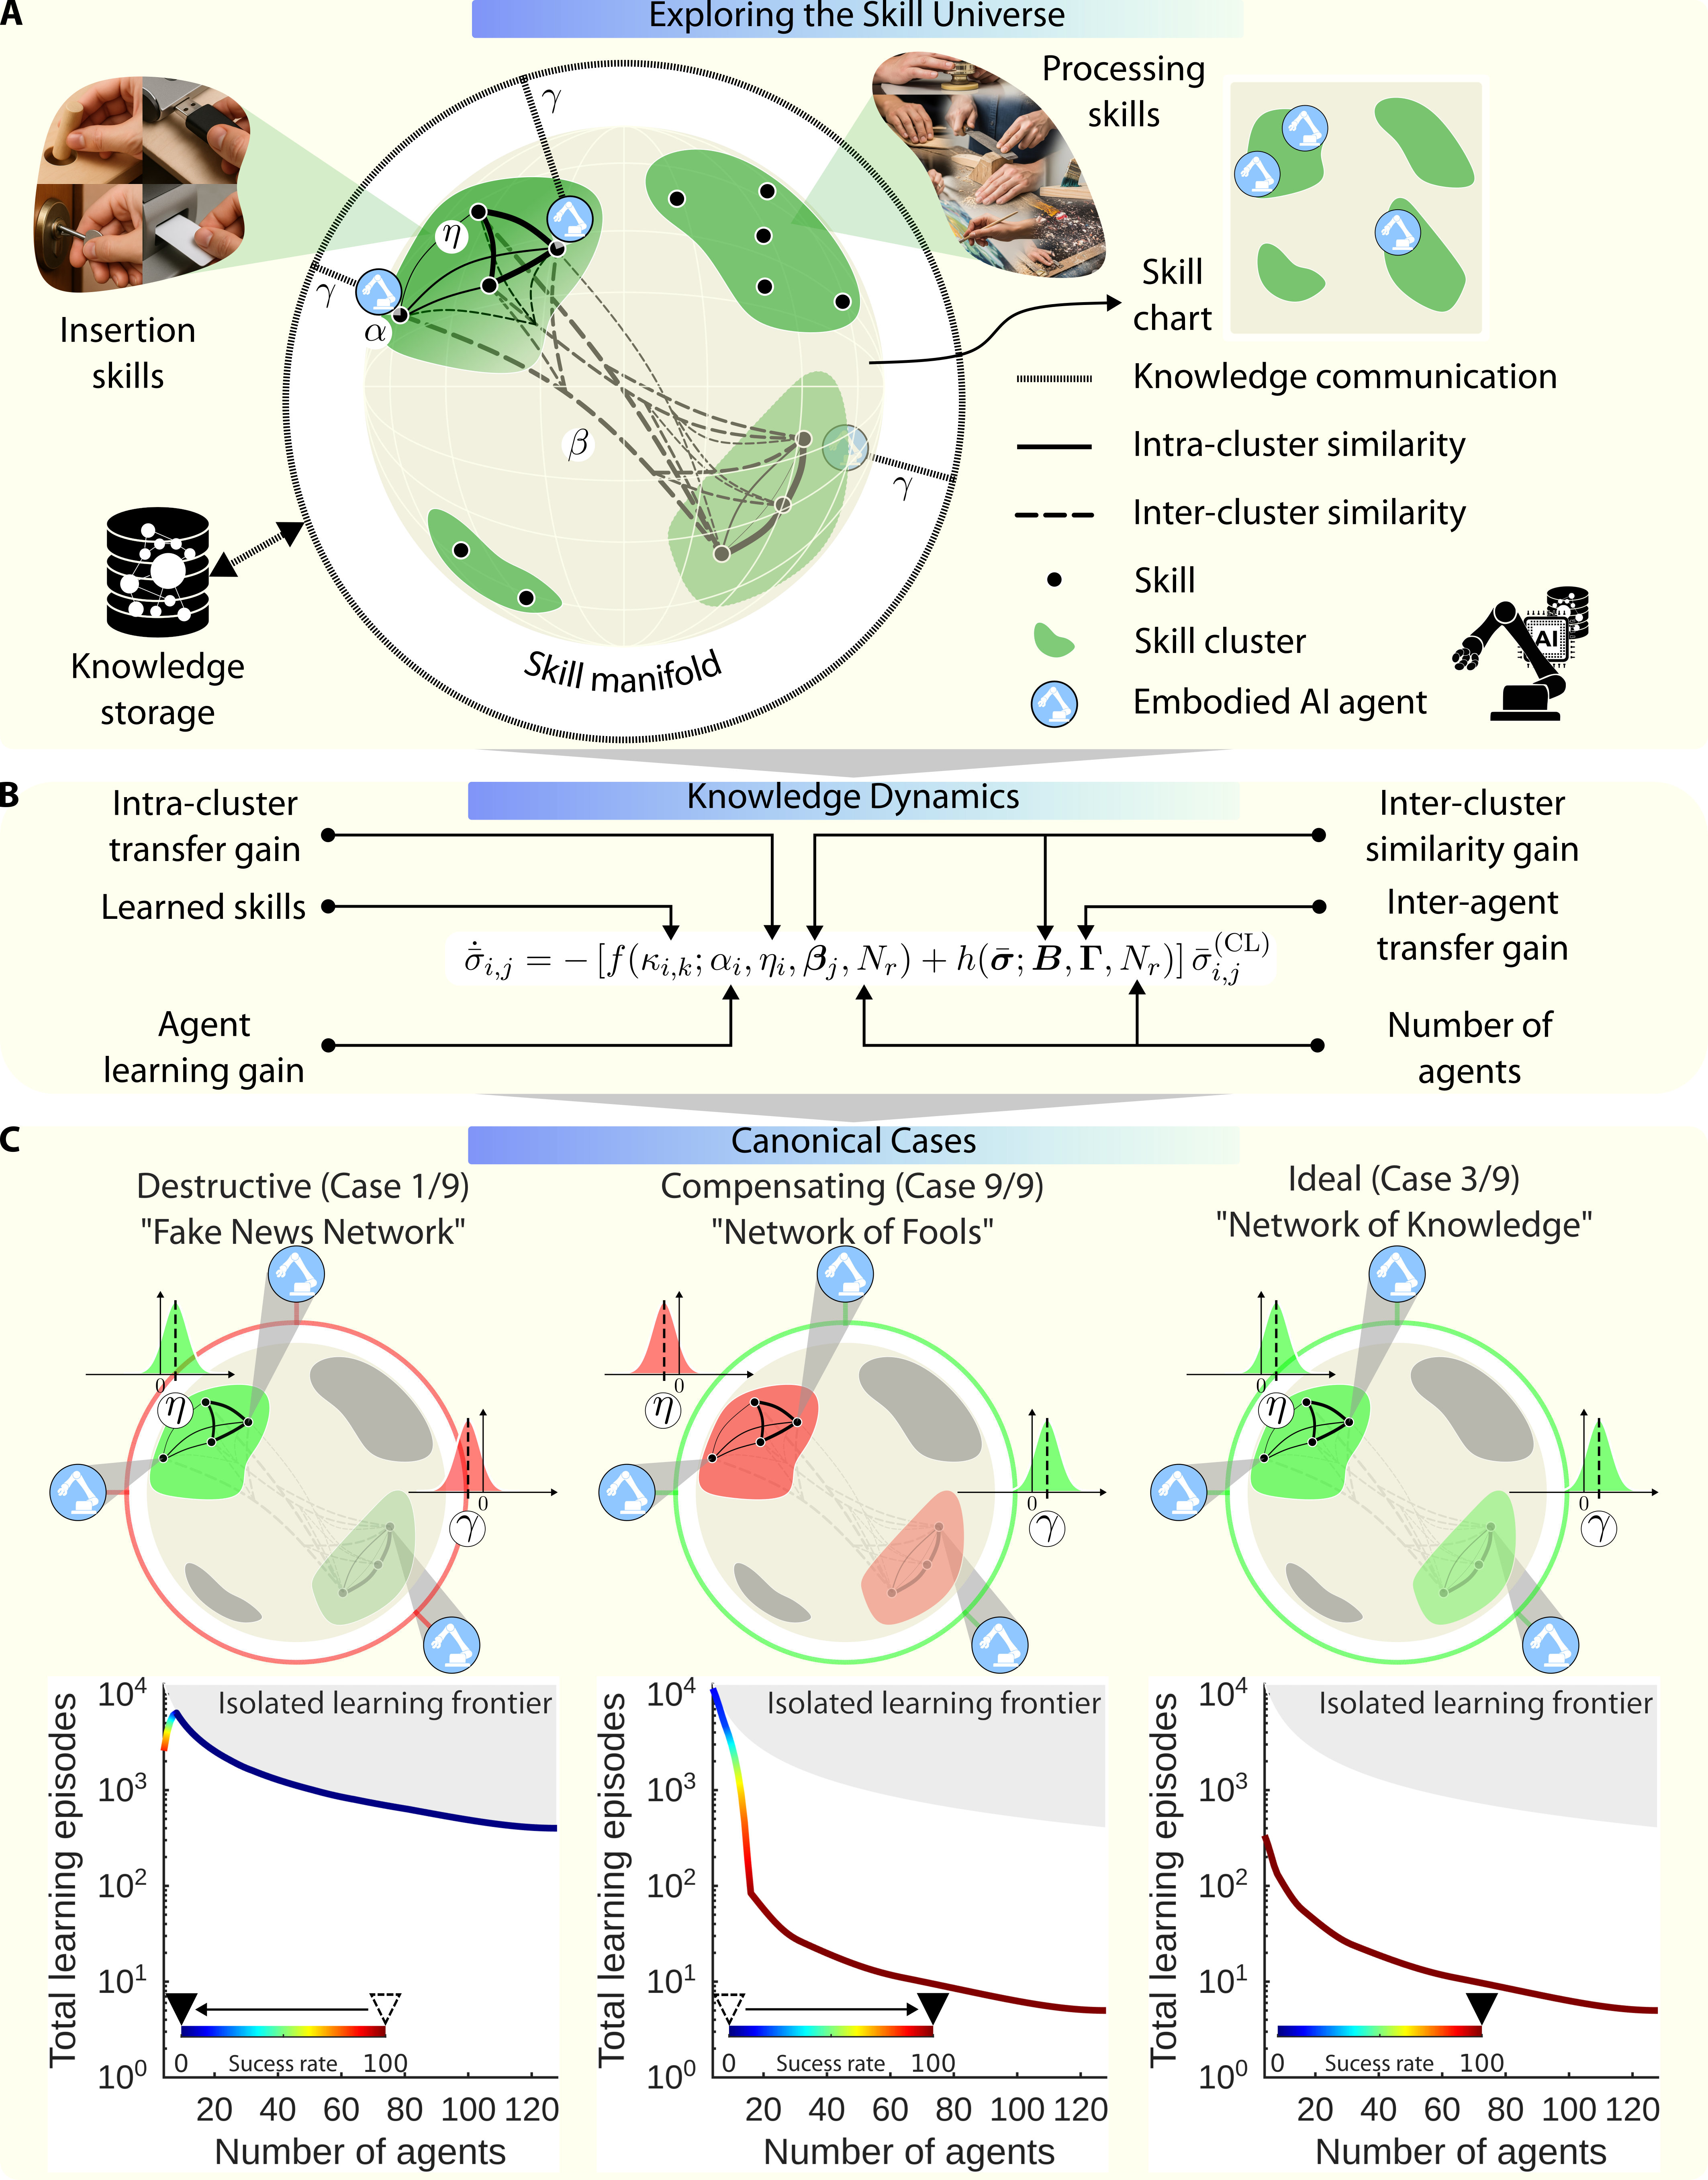
\includegraphics[width=13cm]{collective_learning_and_skill_manifold_conceptualization.png}
	\hspace*{\fill}
    \caption{\label{fig:collective_learning_and_skill_manifold_conceptualization} 
    	% \textbf{Collective learning dynamics over an unknown structured skill manifold.} 
    	% (\textbf{A}) \ac{eai} agents learn and share knowledge across a structured---however, inherently unknown---\textit{skill manifold}, where skills form clusters with intra- and inter-cluster similarity. (\textbf{B}) The skill remaining knowledge dynamics $\dot{\bar{\sigma}}^{(\mathrm{CL})}_j$. (\textbf{C}) Three canonical \ac{cl} regimes: \textit{Destructive}, learning inhibited by poor communication); \textit{Compensating}, weak agents supported by strong network; and \textit{Ideal}, synergistic learning across agents and network.
    	\textbf{Collective learning dynamics over an unknown structured skill manifold.} 
    	(\textbf{A}) \ac{eai} agents learn and share knowledge across a structured---however, inherently unknown---skill manifold. (\textbf{B}) The skill remaining knowledge dynamics $\dot{\bar{\sigma}}^{(\mathrm{CL})}_j$. (\textbf{C}) Three canonical \ac{cl} regimes: \textit{Destructive}---Fake news network---, learning inhibited by poor communication; \textit{Compensating}---network of fools---, weak agents supported by strong network; and \textit{Ideal}---network of knowledge---, synergistic learning across agents and network.        
    }
\end{figure*}
% ---

% ===================================================================================================
\paragraph*{\Acl{cl} of a skill universe}
For an \ac{eai} agent, \emph{data} is generated through interaction, which becomes \emph{information} when patterns and relationships---such as similarities between skills---are extracted during learning. Consequently, \emph{knowledge} is the structured and persistent competence that the agent distills from the acquired information. In this work, we do not aim to characterize knowledge in all its detail, nor to analyze specific individual learning capabilities of \ac{eai} agents or the properties of their network interactions. Instead, we address a fundamental question: \emph{how does inter-agent knowledge sharing shape the dynamics of learning?} by focusing on the general principles that govern collective knowledge integration.

We consider a skill-learning scenario defined as the tuple
% ---
\begin{equation*}
	\phi = \left(N_\mathcal{S}, N_\mathcal{K}, N_\mathrm{r}, \bm{\rho} \right) \in \Phi,
\end{equation*}
% ---
where $N_\mathcal{S}$ is the total number of skills to learn, $N_\mathcal{K}$ is the number of skill clusters, $N_\mathrm{r}$ is the number of \ac{eai} agents, i.e., the size of the collective, and $\Phi$ represents the set of all possible viable combinations. The parameter tuple
% ---
\begin{equation*}
	\bm{\rho} = \left(\bm{\alpha}, \bm{B}, \delta, \bm{\eta},\bm{\Gamma}\right),
\end{equation*}
% ---
defines the knowledge exchange efficiency of the particular scenario; more details about these parameters are provided in \nameref{sec:methods} and depicted in Fig.~\ref{fig:collective_learning_and_skill_manifold_conceptualization}. Notice that the generality of $\Phi$ makes it representative of a variety of scenarios. It can very well be a smart factory setting where multiple robots learn different manufacturing tasks, a home crew of service robots learns different chores, or a fleet of underwater robots performs exploration, inspection, and maintenance routines.

One example of a generic scenario $\phi$ is depicted in Fig.~\ref{fig:collective_learning_and_skill_manifold_conceptualization}, which illustrates a group of robots learning a universe of skills and the associated knowledge dynamics governing \ac{cl} in \ac{eai} systems distributed over a skill space with a similarity-based inherent structure. The notion of a \textit{skill manifold} $\mathcal{S}$ is shown in Fig.~\ref{fig:collective_learning_and_skill_manifold_conceptualization}~\textbf{A}, a structured latent space that represents the underlying similarity structure of a population of $N_\mathcal{S}$ skills. Individual skills group into $N_\mathcal{K}$ \emph{skill clusters} (green patches) based on their shared similarity metrics. For example, insertion tasks (left) and processing tasks (right) may form two distinct but internally (unobservable) coherent skill clusters.
 
%A \emph{robot collective}, namely
%% ---
%\begin{definition}\label{def:robot_collective}
%    a number $N_\mathrm{r}$ of \ac{eai} agents that traverse the skill manifold (without necessarily knowing the structure), each equipped with an ad hoc \ac{ai} algorithm that exploits skill similarity to learn and store skill knowledge, and communication capabilities to integrate and exchange such knowledge with the other peers.
%\end{definition}
%% ---

\begin{definition}\label{def:robot_collective}
	A \emph{robot collective} is a group of $N_\mathrm{r}$ \ac{eai} agents that explore the skill manifold (without requiring prior knowledge of its structure). Each agent is equipped with an ad hoc \ac{ai} algorithm that leverages skill similarity to learn and store knowledge, as well as communication capabilities to exchange and integrate this knowledge with other peers.
\end{definition}

\noindent Solid black lines connecting skills in Fig.~\ref{fig:collective_learning_and_skill_manifold_conceptualization}~\textbf{A} denote \textit{intra-cluster similarity}, promoting efficient incremental accumulation of knowledge from similar skills, while dashed lines linking clusters indicate \textit{intra-cluster similarity}, allowing more challenging but valuable cross-domain knowledge transfer, if performed successfully. Communication among agents and global knowledge storage allow concurrent knowledge accumulation, integration, and exchange of skills within and across clusters.

The expression shown in Fig.~\ref{fig:collective_learning_and_skill_manifold_conceptualization}~\textbf{B}---and detailed in Eq.~\eqref{eq:collective_knowledge_dynamics} in \nameref{sec:methods}---describes the dynamics of the to-be-learned knowledge $\dot{\bar{\sigma}}^{(\mathrm{CL})}_{i,j}$ about a skill~$j$ learned by an \ac{eai} agent~$i$ operating within a \ac{cl} system. This equation depends on four key parameters that govern system behavior. The \textbf{agent learning gain} $\alpha_i \sim \mathcal{U}(\alpha_{\text{min}},\alpha_{\text{max}}) \in \mathbb{R}_+$ captures the embodiment-dependent inherent ability of agent~$i$ to acquire knowledge about skill~$j$ in isolation; the learning gains across all agents are collected in the vector~$\bm{\alpha}$, with the range $[\alpha_{\text{min}}, \alpha_{\text{max}}]$ assumed to be narrow (according to Asm.~\ref{assumption:agent_similarity}). The \textbf{intra-cluster knowledge sharing gain} $\eta_i \sim \mathcal{N}(\bar{\eta},\eta_{\Sigma})$ quantifies how effectively agent~$i$ can reinforce a skill~$j$ through memory of related skills in the same cluster; the vector~$\bm{\eta}$ aggregates these gains across agents and models the efficient reuse of experience, such as accessing stored subskills $\zeta_k$ to support composite skills $s_{j,k}$. The structural similarity within the skill manifold is captured in the \textbf{inter-cluster similarity matrix} $\bm{B} \in \mathbb{R}^{N_\mathcal{K} \times N_\mathcal{K}}$; a corresponding vector~$\bm{\beta}_{ij}$ weighs the contribution of skills from other clusters in the agent’s local memory to the learning of a new skill~$j$. Finally, the \textbf{inter-agent transfer gains} $\gamma_{j,l} \sim \mathcal{N}(\bar{\gamma},\gamma_\Sigma)$, aggregated in the matrix~$\bm{\Gamma} \in \mathbb{R}^{N_\mathrm{r} \times N_\mathrm{r}}$, model the flow of knowledge between agents, accounting for embodiment differences, communication noise, and variation in prior experience. In addition to these four interaction terms, the model includes the intrinsic intelligence $\delta \in (0,\delta_{\text{max}}]$ of the system, controlling also the \textbf{exponential depletion rate} of initially available knowledge.

In addition, the \textbf{number of learned skills}~$\kappa_{i,k}$ from each cluster~$k$ retained in agent~$i$’s memory also influences the dynamics, affecting the knowledge acquisition rate of a skill and the corresponding initial knowledge. Collectively, the parameters $\bm{\rho}$ determine whether the residual knowledge about a skill decreases---indicating successful learning---or increases, which may signal knowledge corruption or forgetting, depending on both individual and collective learning processes.

% ===================================================================================================
\paragraph*{Knowledge dynamics from different learning paradigms}
% In this work, we distinguish learning paradigms in \ac{eai} according to how knowledge is acquired and shared across skills. For the subsequent discussion, in \ac{isl}, agents learn each skill from scratch without reusing prior knowledge. Likewise, we consider \ac{il} as the process in which skill acquisition reuses knowledge from similar, previously learned intra-cluster skills, thereby improving efficiency. \Ac{tl}, on the other hand, considers inter-cluster knowledge reuse, where prior knowledge from one or more origin clusters accelerates skill acquisition in a destination cluster. This process is governed by the \emph{transferable knowledge fractions} $\xi_k$ and $\bar{\xi}_k$, which depend on the cluster similarity matrix $\bm{B}$. The combined use of \ac{il} and \ac{tl}, termed \ac{til}, leverages both intra- and inter-cluster generalization. Further details about these paradigms are provided in \nameref{sec:methods} and in the \nameref{sec:supplementary_materials} Sec.~\ref{sec:conventional_learning_paradigms}.

% In the conventional paradigms, parallelization allows multiple agents to acquire knowledge concurrently, yet aggregation of such knowledge remains impossible due to the absence of inter-agent communication. By contrast, \acl{cl} goes beyond mere parallelization, enabling a collective of $N_\mathrm{r}$ robots to build a shared knowledge base through real-time communication—combining vertical transfer of prior knowledge with horizontal sharing of ongoing experiences. 

% \myhl{It is worth mentioning how our definitions contract with common acceptations in the machine learning research community. Incremental learning is usually referred to as sequential updates to prevent forgetting; likewise, transfer learning is referred to as knowledge reuse across domains via pretraining and fine-tuning. In our framework, however, these notions are rather structural: incremental learning corresponds to intra-cluster reuse, where the acquisition rate scales with the number of learned skills, while transfer learning corresponds to inter-cluster reuse, governed by transferable knowledge fractions and the similarity matrix. A comparison table describing these differences is available in the \nameref{sec:supplementary_materials}.}

We distinguish learning paradigms in \ac{eai} according to how knowledge is acquired and reused across skills. In \ac{isl}, each skill is learned independently from scratch, without leveraging prior experience. By contrast, \ac{il} denotes the reuse of knowledge from similar, previously mastered intra-cluster skills, thereby improving efficiency through structural similarity. \Ac{tl} extends this principle to inter-cluster reuse, where knowledge from one or more origin clusters accelerates learning in a destination cluster. This process is governed by the \emph{transferable knowledge fractions} $\xi_k$ and $\bar{\xi}_k$, which are determined by the cluster similarity matrix $\bm{B}$. The combined paradigm, \ac{til}, exploits both intra- and inter-cluster generalization. Details on the mathematical formalization of these paradigms are provided in \nameref{sec:methods} and further illustrated in the \nameref{sec:supplementary_materials} (Sec.~\ref{sec:conventional_learning_paradigms}).

In the conventional paradigms, parallelization allows multiple agents to learn simultaneously, but aggregation of their knowledge remains impossible without communication. By contrast, \acl{cl} goes beyond parallel learning: a collective of $N_\mathrm{r}$ robots builds a shared knowledge base through real-time communication, combining vertical transfer of prior knowledge with horizontal sharing of ongoing experiences. \myhl{Under a \ac{cl} scheme, the \ac{eai} agents operate in a regime of \ac{slad}, where skill knowledge is integrated collectively through ongoing interaction. We further elaborate on our structural reinterpretation of incremental and transfer learning—contrasting it with the procedural conventions of machine learning—in the \nameref{sec:discussion}, where we also situate the recent advances of foundation models within our knowledge dynamics framework.}

% As an analogy, one may view reinforcement learning as an \ac{il} setting: new data (experiences) continually refine the policy, albeit with respect to a specific reward function. While recent advances in large language models, vision–language(-action) models, and foundation models are often described in terms of \ac{il} or \ac{tl} in the form of generalist policies that are later fine-tuned for a specific task. However, their mechanisms differ from the paradigms considered here. Foundation models are pre-trained over vast data universes (e.g., natural language, multi-modal, and cross embodiment) and can be adapted to related domains via prompting, fine-tuning, or retrieval-augmented extensions. Yet this form of adaptation does not amount to \ac{il} within a domain, nor to structured \ac{tl} across domains in the conventional sense. Instead, it is better understood as large-scale pattern matching or mimicry: correlations captured in one representational universe can be repurposed in another, without explicit representation of the underlying skills. In this sense, foundation models provide powerful statistical generalization, but fall short of the systematic, knowledge-level reuse characteristic of incremental or transfer learning in \ac{eai}.


% In contrast, recent advances in large language models, vision-language(-action) models, and foundation models illustrate a different form of generalization. Rather than incremental refinement or classical transfer, they exploit massive-scale pretraining to capture a broad “skill universe,” and then adapt to new domains primarily through interface-level adjustments (e.g., fine-tuning, prompting, retrieval augmentation). This can be seen less as learning new skills incrementally and more as leveraging pattern matching across structurally similar universes—a form of large-scale mimicry rather than deep incremental knowledge accumulation.



% \paragraph*{Knowledge dynamics from different learning paradigms}
% Learning paradigms in \ac{eai} differ in how knowledge is acquired and shared across skills. In \ac{isl}, agents learn each skill from scratch without reusing prior knowledge. \Ac{il} enables skill acquisition by reusing knowledge from similar, previously learned intra-cluster skills, improving learning efficiency. \Ac{tl} introduces inter-cluster knowledge reuse, where prior knowledge from one or more origin clusters accelerates learning of skills in a destination cluster, governed by the \emph{transferable knowledge fractions} $\xi_k$ and $\bar{\xi}_k$ (which depend on the cluster similarity matrix $\bm{B}$). The combined use of \ac{il} and \ac{tl}, termed \ac{til}, leverages both intra- and inter-cluster generalization. Further details about these paradigms are provided in \nameref{sec:methods} and in the \nameref{sec:supplementary_materials} Sec.~\ref{sec:conventional_learning_paradigms}. \myhl{One could think of reinforcement learning as an example of an incremental learning problem where new data (experiences) refine the policy, albeit for a specific reward. On the other hand, recent advances in large language models, vision-language, vision-language-action models, and foundation models in general display transfer \textcolor{red}{SAMI: discuss, I actually am not sure, I would say they display a sort of transfer, but not in the "transfer learning sense" nor in the "incremental learning", and "fine-tuning" is entirely someting else, I would say they are a very special case of transfer learning: given I have learned a very specifici type of skill universe (such as a particular language), then it can be transferred to an analogues skill universe (across domains?) with essentially the same underlying structure (mimickry), where in both cases the essence of the skill as not learned, as incremental and transfer learning within the universe is not possible. This is the pattern matching / mimickry approach to intelligence so that one can "reuse" underlying models with some "interface/token" tweeking / RAG models to somehow rectifiy the otherwise skewed mapping. In other words, foundation model is mimickry on steroids so we get pretended intelligence, but it is indeed a huge next best response loockup response.} with incremental learning capabilities in the form of generalist policies that are later fine-tuned for a specific task. In the conventional learning paradigms, parallelization allows for concurrent inter-cluster knowledge acquisition, yet aggregation of such knowledge is prevented by the lack of inter-agent communication.} In contrast, \acl{cl} goes beyond mere parallelization, enabling a collective of $N_\mathrm{r}$ robots to build a shared knowledge base through real-time communication, combining vertical transfer of prior knowledge and horizontal sharing of ongoing experiences.

% % ---
% \begin{table}[!t]
% 	\caption{The dynamics of the learning paradigms.\label{tab:learning_paradigms_expressions}}
% 	\begin{center}
% 		\begin{adjustbox}{width=\textwidth}
% 			\begin{tabular}{|l||*{4}{c|}}\hline
% 				\textbf{Learning paradigm}
% 				&\makebox[3em]{\textbf{\ac{isl}}}&\makebox[3em]{\textbf{\ac{il}}}&\makebox[3em]{\textbf{\ac{til}}}
% 				&\makebox[3em]{\textbf{\ac{cl}}}\\\hline\hline
% 				Learning rate  &$ -\alpha_i$ & $ -\alpha_i\left(\eta_i \kappa_{i,k} + 1 \right)$ & -$\alpha_i \left( \frac{\eta_i \kappa_{i,k} + 1}{1 - \xi_k} \right)$ & $  -\alpha_i \left( \frac{\eta_i \kappa_{i,k} + 1}{1 - \xi_k} \right)  - \sum_{l \in \mathcal{N}(j)}\bar{\xi}_{j,l}\gamma_{j,l}d(\cdot)$ \\\hline
% 				Initial condition &$1$ & $e^{-\delta \kappa_{i,k}}$ & $(1-\xi_k) e^{-\delta \kappa_{i,k}}$ & $(1-\xi_k) e^{-\delta \kappa_{i,k}} $ \\\hline
% 			\end{tabular}
% 		\end{adjustbox}
% 	\end{center}	
% \end{table}
% % ---

% ---
\begin{table}[!t]
    \caption{The dynamics of the remaining knowledge for the considered learning paradigms.\label{tab:learning_paradigms_expressions}}
    \begin{center}
        \begin{adjustbox}{width=\textwidth}
            % \begin{tabular}{
            %     >{\raggedright\arraybackslash}p{4.5cm} 
            %     *{4}{>{\centering\arraybackslash}p{3.5cm}}
            % }
            \begin{tabular}{
                >{\raggedright\arraybackslash}p{3cm} 
                *{3}{>{\centering\arraybackslash}p{3cm}}
                *{1}{>{\centering\arraybackslash}p{6.5cm}}
            }            
                \toprule
                \textbf{Learning Paradigm} 
                & \textbf{\ac{isl}} 
                & \textbf{\ac{il}} 
                & \textbf{\ac{til}} 
                & \textbf{\ac{cl}} \\
                \midrule
                Learning rate 
                & $-\alpha_i$ 
                & $-\alpha_i\:\left(\eta_i \kappa + 1 \right)$ 
                & $-\alpha_i\:\left( \frac{\eta_i \kappa + 1}{1 - \xi_{i,j}(\cdot)} \right)$ 
                & $-\alpha_i\:\left( \frac{\eta_i \kappa + 1}{1 - \xi_{i,j}(\cdot)} \right) - \sum_{l \in \mathcal{N}(j)}\bar{\xi}_{i,l}(\cdot)\gamma_{i,l}d(\cdot)$ \\
                \addlinespace[0.5ex]
                Initial condition 
                & $1$ 
                & $e^{-\delta \kappa}$ 
                & $\left(1-\xi_{i,j}(\cdot)\right)\: e^{-\delta \kappa}$ 
                & $\left(1-\xi_{i,j}(\cdot)\right)\: e^{-\delta \kappa}$ \\
                \bottomrule
            \end{tabular}
        \end{adjustbox}
    \end{center}
\end{table}
% ---

To rigorously compare the knowledge acquisition capabilities of the different learning paradigms, we discovered Eq.~\eqref{eq:collective_knowledge_dynamics} as a unifying model that captures the dynamics of the remaining knowledge to be learned under each case. This compositional formulation allowed us to explicitly derive the fundamental differences in isolated, incremental, transfer, and collective learning, and in particular, how the transition from \ac{il} to \ac{cl} dynamics emerges from additional inter-agent knowledge exchange terms. The resulting closed-form expressions for all paradigms, summarized in Table~\ref{tab:learning_paradigms_expressions}, provide a direct analytical basis to quantify and contrast their efficiency.

% In summary, the model parameters have the following interpretations:
% % ---
% \begin{enumerate}
% 	\item The parameter $\alpha_i \sim \mathcal{U}(\alpha_{\text{min}},\alpha_{\text{max}}) \in \mathbb{R}_+$ accounts for different embodiments and models the \emph{base learning rate} at which a robot in isolation learns any given skill. According to Asm.~\ref{assumption:agent_similarity}, the range $[\alpha_{\text{min}},\alpha_{\text{max}}]$ is rather narrow.
% 	\item The parameter $\delta \in (0,\delta_{\text{max}}]$ reflects the intrinsic intelligence of the system and controls the \emph{exponential depletion rate}  of the initial remaining knowledge.
% 	\item The parameter $\eta_i \sim \mathcal{N}(\bar{\eta},\eta_{\Sigma})$ is the \emph{intra-cluster knowledge exchange factor}, it models the efficient use of experience (e.g. accessing memory) and represents the efficiency of knowledge exchange from $\zeta_k$ to $s_{j,k}$.
% 	\item The parameter $\gamma_{j,l} \sim \mathcal{N}(\bar{\gamma},\gamma_\Sigma)$ is the \emph{inter-agent knowledge exchange factor}, it weighs the knowledge exchange between agents and accounts for different embodiments, false communication, and dissimilar knowledge.
% %	\item $\beta_k$ is the head start granted by knowledge transfer from other clusters to the skills in $\mathcal{Z}_k$.
% \end{enumerate}
 
% In \ac{cl}, the dynamics of the remaining knowledge  about a skill acquired by an agent exchanging knowledge with a set $\mathcal{N}$ of other agents is described by
% % ---
% \begin{equation}\label{eq:collective_knowledge_dynamics}
% 	\dot{\bar{\sigma}}^{(\text{CL})}_{j,k} =
% 		\overbrace{\left[-\alpha \left( \frac{\eta \kappa + 1}{1 - \xi_k} \right)  - \sum\limits_{l \in \mathcal{N}(j)} \bar{\xi}_{j,l} \gamma_{j,l} d(\bar{\sigma}_j,\bar{\sigma}_l)\right]}^{f(\cdot)} \bar{\sigma}^{(\text{CL})}_{j,k},
% \end{equation}
% % ---

% \noindent for $\epsilon < \bar{\sigma}_{j,k} < 1$ and with initial conditions $\bar{\sigma}^{(\text{CL})}_{j,k}(0) = g_{j,k}\left(\kappa\right)$. Note that $\kappa$ represents the total number of successfully learned skills. Each gain $\gamma_{j,l} \in \mathbb{R} $ weighs the knowledge exchange strength among robots. Since robots may have in-memory skills from different clusters, the transferable knowledge fraction factor
% % ---
% \begin{equation} 
% 	\bm{\xi} = [\xi_1 \cdots \xi_k \cdots \xi_{N_\mathcal{K}}]^\intercal = (\bm{B} - \bm{I}) \bm{\varsigma} ,
% \end{equation}
% % ---
% with $\bm{\varsigma} \in \mathbb{R}^{N_\mathcal{K}}$; accounts for the one-time transfer of knowledge based upon the cluster similarity at the beginning of a learning cycle. Similarly, the term $ \bar{\xi}_{j,l} $ scales the concurrent---that is, during learning---sharing of knowledge coming from the skills currently being learned in different clusters. The functions
% % ---
% \begin{equation}\label{eq:f_function_collective}
% 	f(\cdot) = -\alpha \left( \frac{\eta \kappa + 1}{1 - \xi_k} \right)  - \sum_{l \in \mathcal{N}(j)} \bar{\xi}_{j,l} \gamma_{j,l}d(\bar{\sigma}_j,\bar{\sigma}_l)
% \end{equation}

% % --- 
% \noindent and 
% % ---
% \begin{equation}%\label{eq:f_function_collective}
% 	g(\cdot) = (1-\xi_k) e^{-\delta \kappa}
% \end{equation}
% % ---
% \noindent are dependent on the number of successfully learned skills $ \kappa $ and the $N_\mathrm{r}$ knowledge-exchanging robots. Note that, after a learning cycle, ideally $\kappa= N_\mathrm{r} N_{\zeta_k}$; however, since some agents may fail to successfully learn a given skill, then $\kappa \leq N_\mathrm{r} N_{\zeta_k}$.

% The \emph{knowledge integration function} 
% % ---
% \begin{equation}\label{eq:knowledge_integration_function}
% 	d(\bar{\sigma}_j,\bar{\sigma}_l) = e^{-a\left(\bar{\sigma}_l-\bar{\sigma}_j\right)^2}\in [0,1],
% \end{equation}
% % --- 
% \noindent in Eq.~\eqref{eq:collective_knowledge_dynamics} accounts for the contribution of knowledge from other agents, weighing it according to the relevance (similarity) of the shared knowledge. 







% In this work, our focus is not on the individual capabilities of the agents nor on the various topologies and associated properties of their networked interactions. Rather, we address a deeply fundamental question: \emph{what if the learning paradigm enables inter-agent knowledge sharing?} We consider a skill-learning scenario defined as the tuple
% % ---
% \begin{equation*}
% 	\phi = \left(N_\mathcal{S}, N_\mathcal{K}, N_\mathrm{r}, \bm{\rho} \right) \in \Phi,
% \end{equation*}
% % ---
% where $N_\mathcal{S}$ is the total number of skills to learn, $N_\mathcal{K}$ is the number of skill clusters, $N_\mathrm{r}$ is the number of \ac{eai} agents, i.e., the size of the collective, and $\Phi$ represents the set of all possible viable combinations. The parameter tuple
% % ---
% \begin{equation*}
% 	\bm{\rho} = \left(\bm{\alpha}, \bm{B}, \delta, \bm{\eta},\bm{\Gamma}\right),
% \end{equation*}
% % ---
% defines the knowledge exchange efficiency of the particular scenario, more details about these parameters are provided in \nameref{sec:methods}. Notice that the generality of $\Phi$ makes it representative of a variety of scenarios. It can very well be a smart factory setting where multiple robots learn different manufacturing tasks, a home crew of service robots learns different chores, or a fleet of underwater robots performs exploration, inspection, and maintenance routines. %\myhl{The different hypothetical scenarios posed by $\Phi$ allow contrasting the different learning paradigms regarding their associated energy demand (related to the \ac{cce}, \ac{bee}, and \ac{mie} expenditure categories).}

% ===================================================================================================
% \textcolor{blue}{To study the idealized dynamics of a \ac{cl} system, we first discuss a scenario in which each of the $N_\mathrm{r}$ \ac{eai} agents in the collective learns a different skill every learning cycle\footnote{A learning cycle encompasses all the learning episodes required to learn a given skill batch.}. In this idealized scenario, the collective learns $N_\mathcal{S}=512$ skills, segregated into $N_\mathcal{K}=4$ clusters of $N_\mathcal{Z} = 128$ skills each. A given skill, according to Eq.~\eqref{eq:simple_knowledge_dynamics}, is considered learned when the remaining knowledge $\bar{\sigma}$ falls below the threshold $\epsilon$. The fundamental complexity of each skill---the assumed maximum number of episodes to learn it---is $c_0 = 100$ episodes. Finally, for simplicity, the energetic cost of a learning episode is assumed to be constant and is represented by $ e_0 $. Consequently, the total energy expenditure to learn all skills is directly proportional to the total number of learning episodes. Details on the values of the elements in $\bm{\rho}$ are provided in \nameref{sec:supplementary_materials}.}

% \paragraph*{Canonical \acl{cl} regimes}
% \myhl{Recall that $\bar{\eta}$ quantifies the average quality of learning from previous knowledge at the level of individual agents; high $\bar{\eta}$ corresponds to consistent, robust knowledge accumulation within a robot; low $\bar{\eta}$ indicates erratic behavior or even knowledge degradation. Likewise, $\bar{\gamma}$ characterizes the integrity and effectiveness of the collective exchange of knowledge between agents. A high $\bar{\gamma}$ implies stable and constructive accumulation of shared knowledge, while a low $\bar{\gamma}$ may imply knowledge corruption or destruction, for example, due to noisy communication, concept drift, or misaligned objectives.}

% \myhl{Based on the relevant possible combinations of the mean values $\bar{\eta}$ and $\bar{\gamma}$, and using and idealized scenario in which each of the $N_\mathrm{r}$ \ac{eai} agents in the collective learns a different skill every learning cycle\footnote{A learning cycle encompasses all the learning episodes required to learn a given skill batch.}, we discovered nine canonical regimes for a \ac{cl} system. \textbf{Those cases are summarized} in Table~\ref{tab:cl_regimes} and are shown in the performance plots in Fig.~\ref{fig:collective_learning_cases}. These nine rigmies can be }

% Fig.~\ref{fig:collective_learning_and_skill_manifold_conceptualization}~\textbf{C} illustrates three canonical operating regimes of a \ac{cl} system dependent on the mean values $(\bar{\eta}, \bar{\gamma})$. Each regime is visualized through: (i) a schematic of the agent-skill-manifold interaction, (ii) corresponding Gaussian distributions for $\eta$ and $\gamma$, and (iii) a performance plot showing the total learning episodes executed in an attempt to learn all the $ N_\mathcal{S} $ skills as a function of the collective size. The performance plots also include information on the success rate, that is, the percentage of skills actually learned.

% In the \textbf{destructive regime}---dubbed the \emph{``Fake News Network''}---competent agents (\(\bar{\eta} > 0\)) are undermined by misleading or noisy collective interactions (\(\bar{\gamma} < 0\)). The collective behavior of the system amplifies the propagation of errors, resulting in a degradation of learning efficiency despite agent-level capabilities. %As shown in the learning frontier plot, performance plateaus with increasing agent count.
% ~In the \textbf{compensating regime} (the \emph{``Network of Fools''}), agents exhibit negative learning dynamics (\(\bar{\eta} < 0\)), but a well-functioning collective with high $\bar{\gamma}$ counteracts this deficit. Collective robustness enables scalable improvement, with the number of learning episodes significantly decreasing with the size of the collective. Finally, in the \textbf{ideal regime}, \emph{``Network of Knowledge''}, both the agent and the collective components contribute positively (\(\bar{\eta} > 0, \bar{\gamma} > 0\)), leading to synergistic \acl{cl}. This regime achieves the steepest reduction in total learning episodes as more agents are added, exemplifying highly energy-efficient distributed skill acquisition.

% ---
\begin{figure*}[t!]
	\centering
	\hspace*{\fill}
	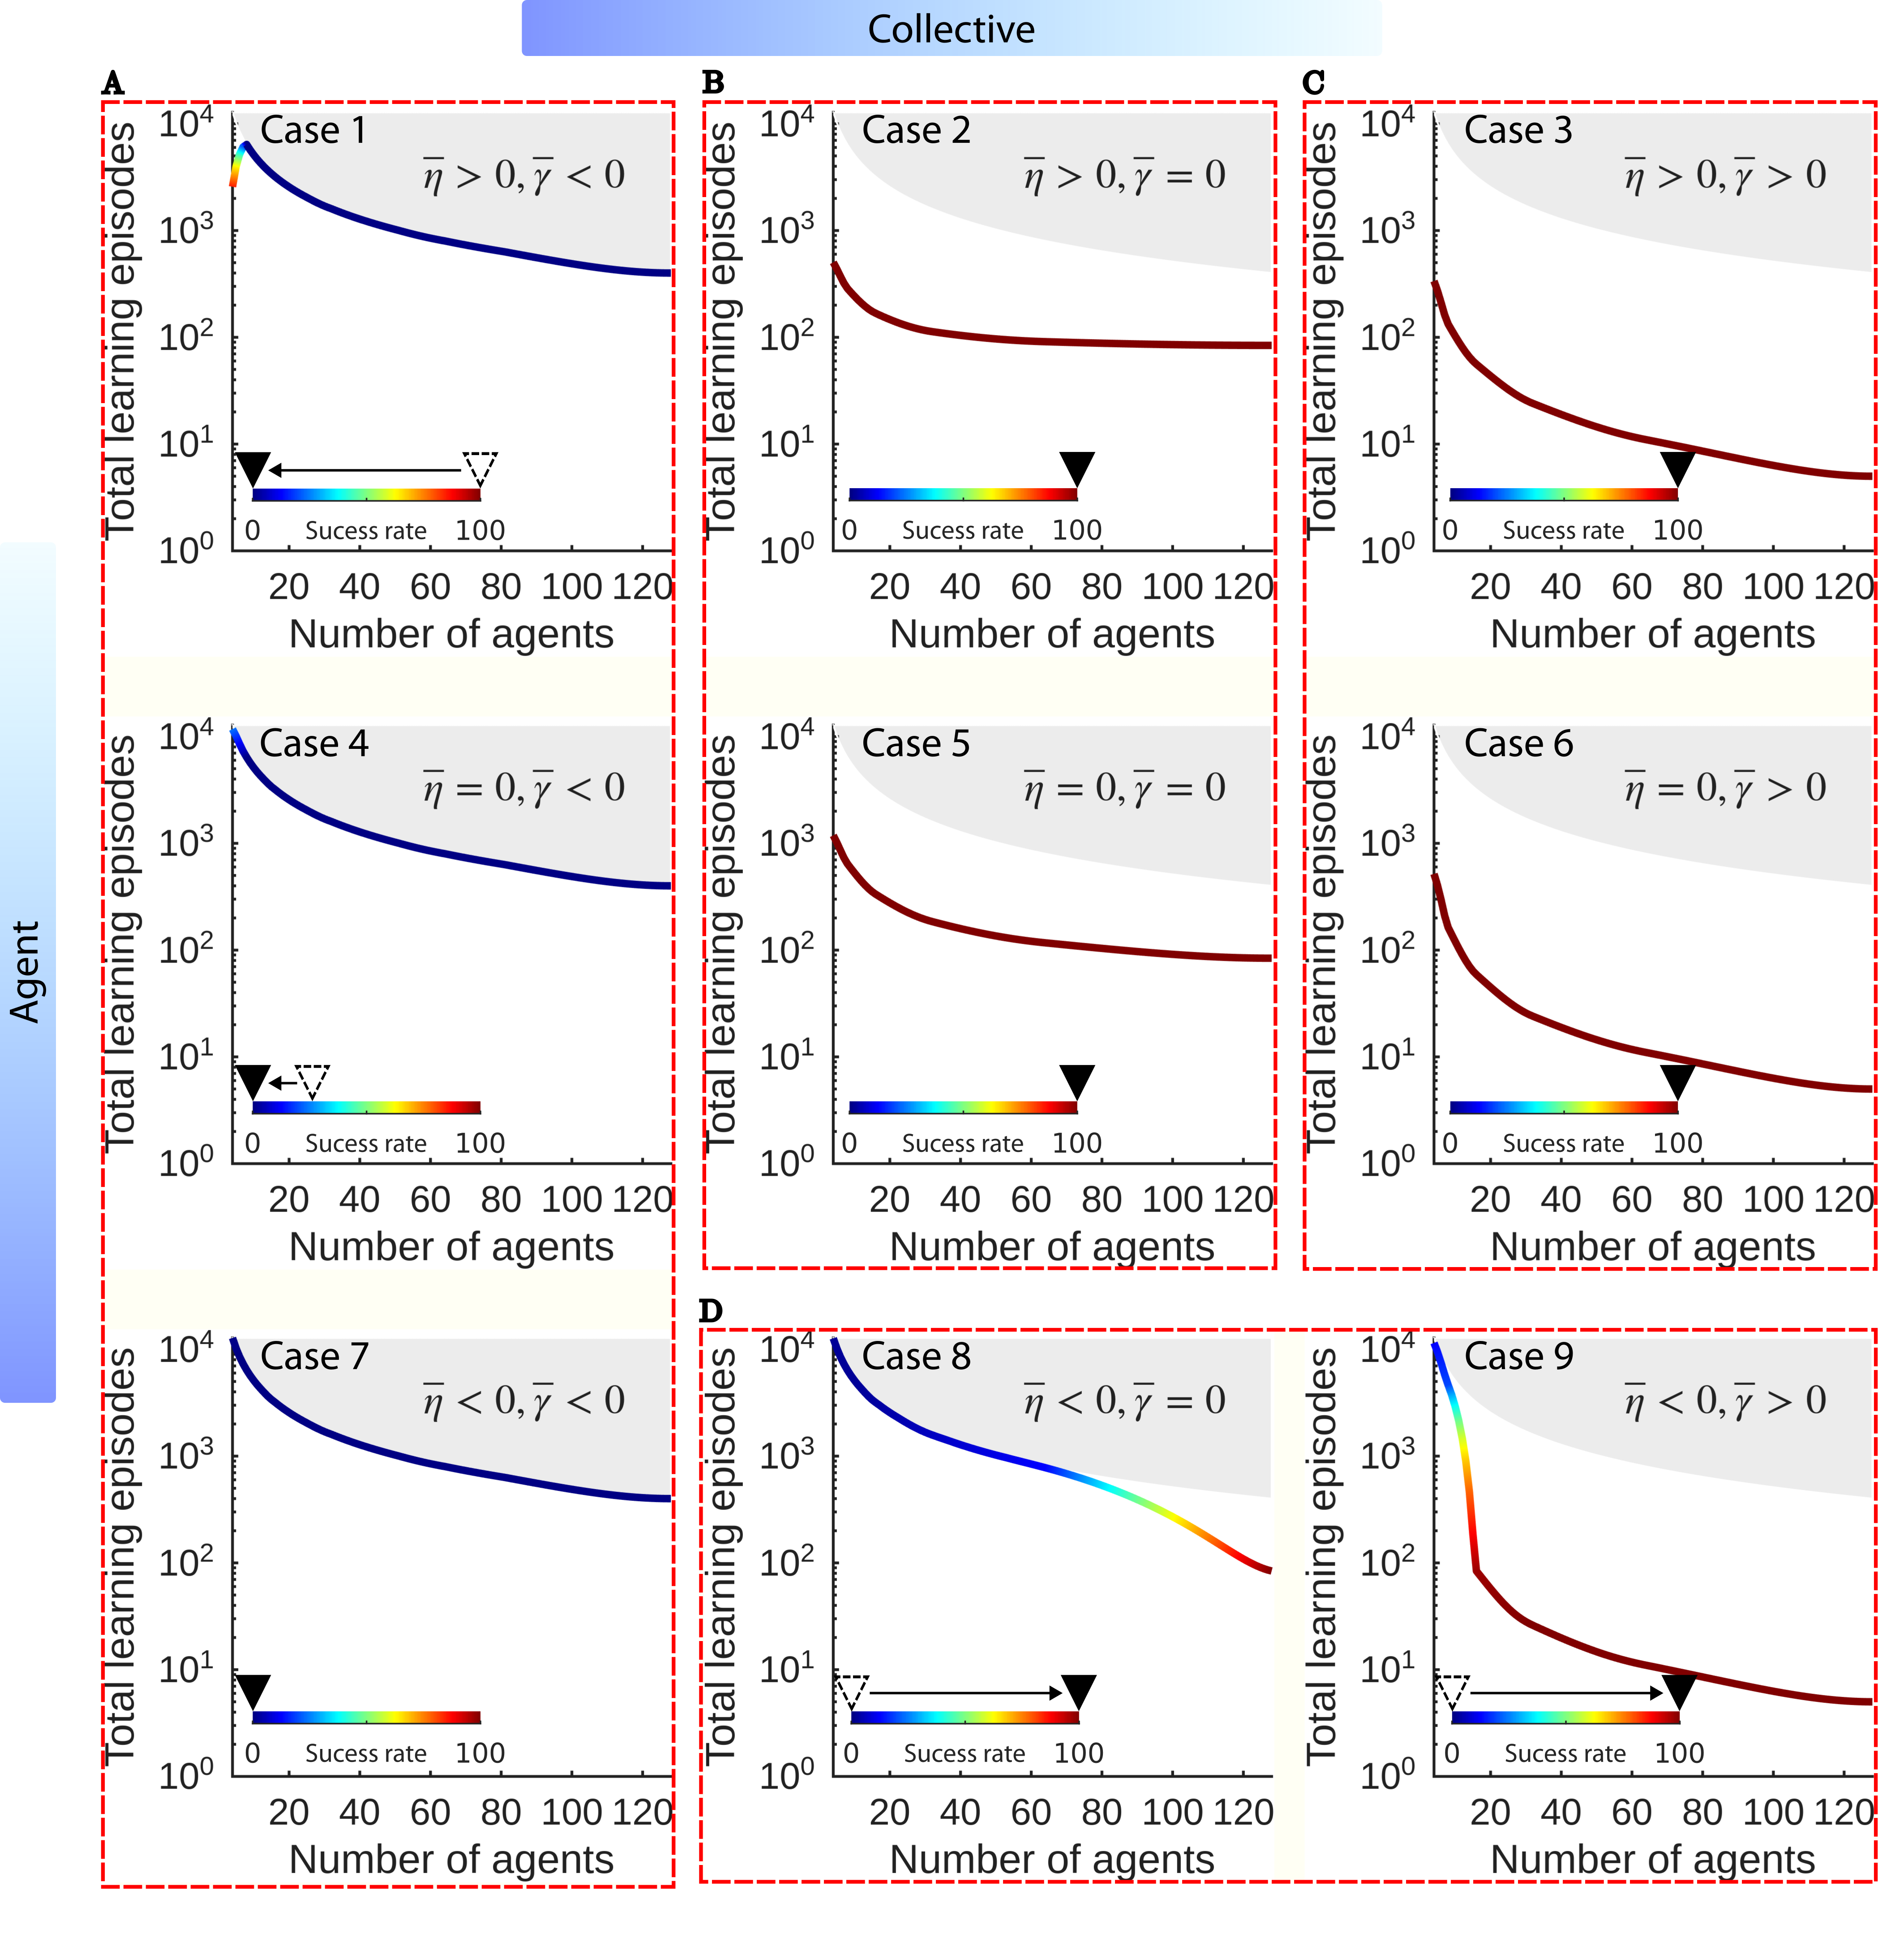
\includegraphics[width=14cm]{collective_learning_cases.png}
	\hspace*{\fill}
	% \caption[] {\label{fig:collective_learning_cases} \textbf{Different regimes exhibited by a \acl{cl} system.} {Depending on the mean value of $ \eta $ and $ \gamma $, a robot collective will have different behavior and performance in terms of the total number of episodes (correspondingly, energy) required to learn all skills and the associated success rate (percentage of skills successfully learned). Four canonical regimes are discovered: (\textbf{A}) destructive, (\textbf{B}) canceling, (\textbf{C}) ideal, and (\textbf{D}) compensating network behavior. (\textbf{E} The size of the collective impacts the total learning episodes and the success rate of the \ac{cl}.}}
	\caption[] {\label{fig:collective_learning_cases} \textbf{Canonical regimes of a \acl{cl} system.} Robot collectives exhibit distinct behaviors depending on the mean values of $\eta$ and $\gamma$, affecting the total learning episodes (and thus energy) and success rate. Four principal regimes are identified: (\textbf{A}) destructive, (\textbf{B}) canceling, (\textbf{C}) ideal, and (\textbf{D}) compensating. (\textbf{E}) Collective size influences both learning efficiency and success.}
\end{figure*}
% ---

% ---
\begin{figure*}[t!]
	\centering
	\hspace*{\fill}
	\includegraphics[width=14cm]{cases_point_plot.png}
	\hspace*{\fill}
	\caption[] {\label{fig:cases_point_plot} \textbf{Collective size influences both learning efficiency and success.} The size of the robot collective can steer the learning of the skill universe leveraging the positive influence of $\bar{\gamma}$.}
\end{figure*}
% ---

% % ---
% \begin{table}[t!]
% 	\centering
% 	\caption{\label{tab:cl_regimes} Regimes of a \ac{cl} system.}
% 	\renewcommand{\arraystretch}{1.2}
% 	\begin{tabular}[t]{|l| p{5cm}|}
% 		\hline
% 		\textbf{Case} & \textbf{Description}\\
% 		\hline
% 		Case 1 ($\bar{\eta} >0,~\bar{\gamma}<0$) & {Agent accumulates knowledge, collective destroys knowledge.} \\
% 		\hline
% 		Case 2 ($\bar{\eta} >0,~\bar{\gamma}=0$) & {Agent accumulates knowledge, collective corrupts knowledge.}\\
% 		\hline
% 		Case 3 ($\bar{\eta} >0,~\bar{\gamma}>0$) & {Agent and collective accumulate knowledge.}\\
% 		\hline
% 		Case 4 ($\bar{\eta} =0,~\bar{\gamma}<0$) & {Agent erratically accumulates knowledge, collective destroys knowledge.}\\
% 		\hline
% 		Case 5 ($\bar{\eta} =0,~\bar{\gamma}=0$) & {Agent and collective erratically accumulate knowledge.}\\
% 		\hline
% 		Case 6 ($\bar{\eta} =0,~\bar{\gamma}>0$) & {Agent erratically use previous knowledge and collective shares knowledge.}\\
% 		\hline
% 		Case 7 ($\bar{\eta} <0,~\bar{\gamma}<0$) & {Agent and collective destroy knowledge.}\\
% 		\hline
% 		Case 8 ($\bar{\eta} <0,~\bar{\gamma}=0$) & {Agent corrupts knowledge and collective erratically share knowledge.}\\
% 		\hline
% 		Case 9 ($\bar{\eta} <0,~\bar{\gamma}>0$) & {Agent destroys knowledge, collective accumulates knowledge (compensates).}\\
% 		\hline	
% 	\end{tabular}
% 	\label{tab:caption}
% \end{table}%
% ---
% % ---
% \begin{figure*}[t!]
% 	\centering
% 	\hspace*{\fill}
% 	\includegraphics[width=0.95\textwidth]{fig/cases_point_plot.png}
% 	\hspace*{\fill}
% 	\caption[] {\label{fig:cases_point_plot} \textbf{Effect of the collective size on the learning energy and success.} The size of the collective impacts the success rate of the \ac{cl} system depending on the mean values ($\bar{\eta},\bar{\gamma}$) }
% \end{figure*}
% %---
% In case 1, the agent accumulates knowledge, while the collective destroys it. Here, each agent benefits from prior knowledge stored locally, but communication with other agents introduces corruptions that degrade learning; as corrupted knowledge spreads, the overall success rate drops rapidly. In case 2, the agent again accumulates knowledge, but the collective merely corrupts it---competent agents are undermined by a noisy or unreliable network, possibly due to poor synchronization, stale updates, or adversarial sharing. Case 3 represents the ideal regime: both individual and collective learning processes are stable and mutually strengthening, enabling scalable, energy-efficient performance.

% In case 4, the agent's learning is erratic, and the collective exacerbates this instability, leading to inefficiencies or fragmented knowledge. Case 5 is similarly unstable, but some learning still occurs; such behavior may stem from partial observability, asynchronous updates, or sparse data, and may be stabilized through robust system design. In case 6, the agent intermittently leverages past knowledge while the collective supports learning, leading to successful outcomes at slightly higher complexity compared to Case 3.

% The most adverse behavior arises in case 7, where both the agent and the collective destroy knowledge---an outcome that may result from catastrophic forgetting, model collapse, or uncoordinated behavior. In case 8, the agent corrupts knowledge while the collective shares it erratically; interestingly, a sufficiently large collective can still enable successful learning. Finally, Case 9 describes a compensatory regime where individual agents degrade, but the collective accumulates knowledge effectively, highlighting the potential of fault-tolerant, robust collective systems.

% These nine discovered regimes can be clustered into four principal regimes according to the impact on the success rate: Fig.~\ref{fig:collective_learning_cases}~\textbf{A} destructive network behavior (cases 1, 4, and 7), Fig.~\ref{fig:collective_learning_cases}~\textbf{B} canceling network behavior (cases 2 and 5), Fig.~\ref{fig:collective_learning_cases}~\textbf{C} ideal agent-collective behavior (cases 3 and 6), and Fig.~\ref{fig:collective_learning_cases}~\textbf{C} compensating network behavior (cases 8 and 9). Three of these cases have already been touched on. In the \textbf{canceling regime}, the mean values $\bar{\eta}$ and $\bar{\gamma}$ strike a balance that, while still ensuring successful learning of all skills, it still demands a larger number of learning episodes than the ideal regime, hence significantly more learning energy. In short, the performance plots in Fig.~\ref{fig:collective_learning_cases} provide insight into the energetic demands of the different \ac{cl} regimes, emphasizing that successful knowledge acquisition in \acl{cl} is more dependent on interconnectivity and successful knowledge sharing between agents. This is observed in cases 8 and 9, where even in the presence of meager individual learning capabilities, the size of the collective will lead to successful learning of the skills if the connectivity ensures stable knowledge sharing.

% ===================================================================================================
\paragraph*{Canonical \acl{cl} regimes}
The \acl{cl} behavior of a system depends crucially on two key parameters: the mean intra-agent knowledge retention $\bar{\eta}$ and the mean inter-agent knowledge transfer gain $\bar{\gamma}$. Recall that the parameter $\bar{\eta}$ captures the average quality of learning from prior knowledge at the individual level. Thus, a high $\bar{\eta}$ implies robust and consistent knowledge accumulation within each robot, whereas a low $\bar{\eta}$ signals erratic internal learning or even degradation of stored knowledge. Conversely, $\bar{\gamma}$ characterizes the integrity and effectiveness of knowledge exchange across the agent network. A high $\bar{\gamma}$ enables constructive, reliable sharing of skills, while a low value reflects corruption due to issues like noisy communication, concept drift, or divergent objectives.

To analyze how these two factors shape system-level dynamics, we studied an idealized scenario---the particulars of this scenario are provided in the \nameref{sec:supplementary_materials} Sec.~\ref{sec:results_supplementaries}---where each of the $N_\mathrm{r}$ \ac{eai} agents in the collective learns a different skill in every learning cycle---i.e., all the episodes required to learn a given skill batch. Based on all possible combinations of $\bar{\eta}$ and $\bar{\gamma}$, we identified nine canonical \ac{cl} regimes that can be categorized further into four principal regimes. Fig.~\ref{fig:collective_learning_and_skill_manifold_conceptualization}~\textbf{C} illustrates three of these principal regimes, each depicted through a schematic of agent-skill-manifold interaction, Gaussian distributions over $\eta$ and $\gamma$, and performance plots indicating the number of learning episodes required to acquire all $N_\mathcal{S}$ skills as a function of collective size. It is worth mentioning that, since, for simplicity, the energetic cost $ e_0 $ of a learning episode is assumed to be constant, the total energy expenditure to learn all skills is directly proportional to the total number of learning episodes.

In the \textbf{destructive regime}---referred to as the \emph{``Fake News Network''}---competent agents ($\bar{\eta} > 0$) are misled by faulty collective interactions ($\bar{\gamma} < 0$). Despite having robust internal learning, agents suffer from corrupt external knowledge that spreads rapidly, resulting in reduced system performance. In contrast, the \textbf{compensating regime}, labeled \emph{``Network of Fools''}, features agents with poor internal learning ($\bar{\eta} < 0$) supported by a strong and reliable collective ($\bar{\gamma} > 0$). This collective structure compensates for individual shortcomings, reducing the number of learning episodes with increasing collective size. The \textbf{ideal regime}, or \emph{``Network of Knowledge''}, emerges when both agent-level and network-level learning are stable and constructive ($\bar{\eta} > 0, \bar{\gamma} > 0$). Here, the system achieves maximal efficiency and minimal energy expenditure in distributed skill acquisition.

Beyond these principal regimes, analysis of the individual canonical regimes provides further insight. As visualized in the performance plots of Fig.~\ref{fig:collective_learning_cases}, in \textbf{Case 1}, agents retain knowledge well, but collective communication is destructive. This leads to rapid decay in success rates due to corrupted knowledge propagation. \textbf{Case 2} is similar: agents learn effectively, but the network only partially degrades knowledge—failures may result from misaligned updates, stale messages, or adversarial sharing. \textbf{Case 3} represents the ideal, where both individual and collective learning reinforce each other, yielding scalable and efficient performance. 

In \textbf{Case 4}, both the agents and the collective behave erratically, compounding instability. \textbf{Case 5} shows partial recovery from this: some learning occurs due to stochastic factors or sparse data, which might be stabilized via architectural or procedural improvements. \textbf{Case 6} features agents that intermittently reuse prior knowledge, supported by a cooperative collective—resulting in success, albeit at a higher complexity cost than in Case 3.

\textbf{Case 7} presents the worst scenario, with both agents and the network actively destroying knowledge, possibly due to catastrophic forgetting, model collapse, or uncoordinated learning. In \textbf{Case 8}, agents corrupt knowledge individually, but the network offers some structure; with sufficient scale, even this erratic setting can yield learning. Finally, \textbf{Case 9} demonstrates that even when individual agents degrade knowledge, a robust collective can ensure successful learning through strong knowledge sharing.

As already mentioned, we clustered the nine canonical regimes into four principal regimes, as shown in Fig.~\ref{fig:collective_learning_cases}: \textbf{(A)} destructive regimes (Cases 1, 4, 7), \textbf{(B)} canceling regimes (Cases 2, 5), \textbf{(C)} ideal regimes (Cases 3, 6), and \textbf{(D)} compensating regimes (Cases 8, 9). The \textbf{canceling regime} strikes a delicate balance: while all skills can still be learned, the required number of episodes is significantly higher than in the ideal case, implying a higher energy cost. Overall, the performance plots in Fig.~\ref{fig:collective_learning_cases} emphasize that system-wide success in \acl{cl} depends more on robust inter-agent connectivity and shared knowledge dynamics than on isolated learning capabilities. This is particularly evident in compensating cases (8 and 9), where large collectives overcome individual agent weaknesses through stable, redundant communication structures. To also highlight the influence that the size of the collective has in the different regimes, Fig.~\ref{fig:cases_point_plot} shows the total learning episodes and the success rate, defined as the percentage of skills successfully learned, for all regimes. Depending of parameters ($\bar{\eta},\bar{\gamma}$) the size of the collective can bring the system from a successful learning state to an entire obliteration of the knowledge capability (as in Case 1), while in Cases 8 and 9, the growing size of the collective drives the system towards successful learning of the skill universe, in spite of the individual learning limitations.


% ===================================================================================================
\paragraph*{A smart factory case study}
% ---
\begin{figure*}[t!]
	\centering
	\hspace*{\fill}
	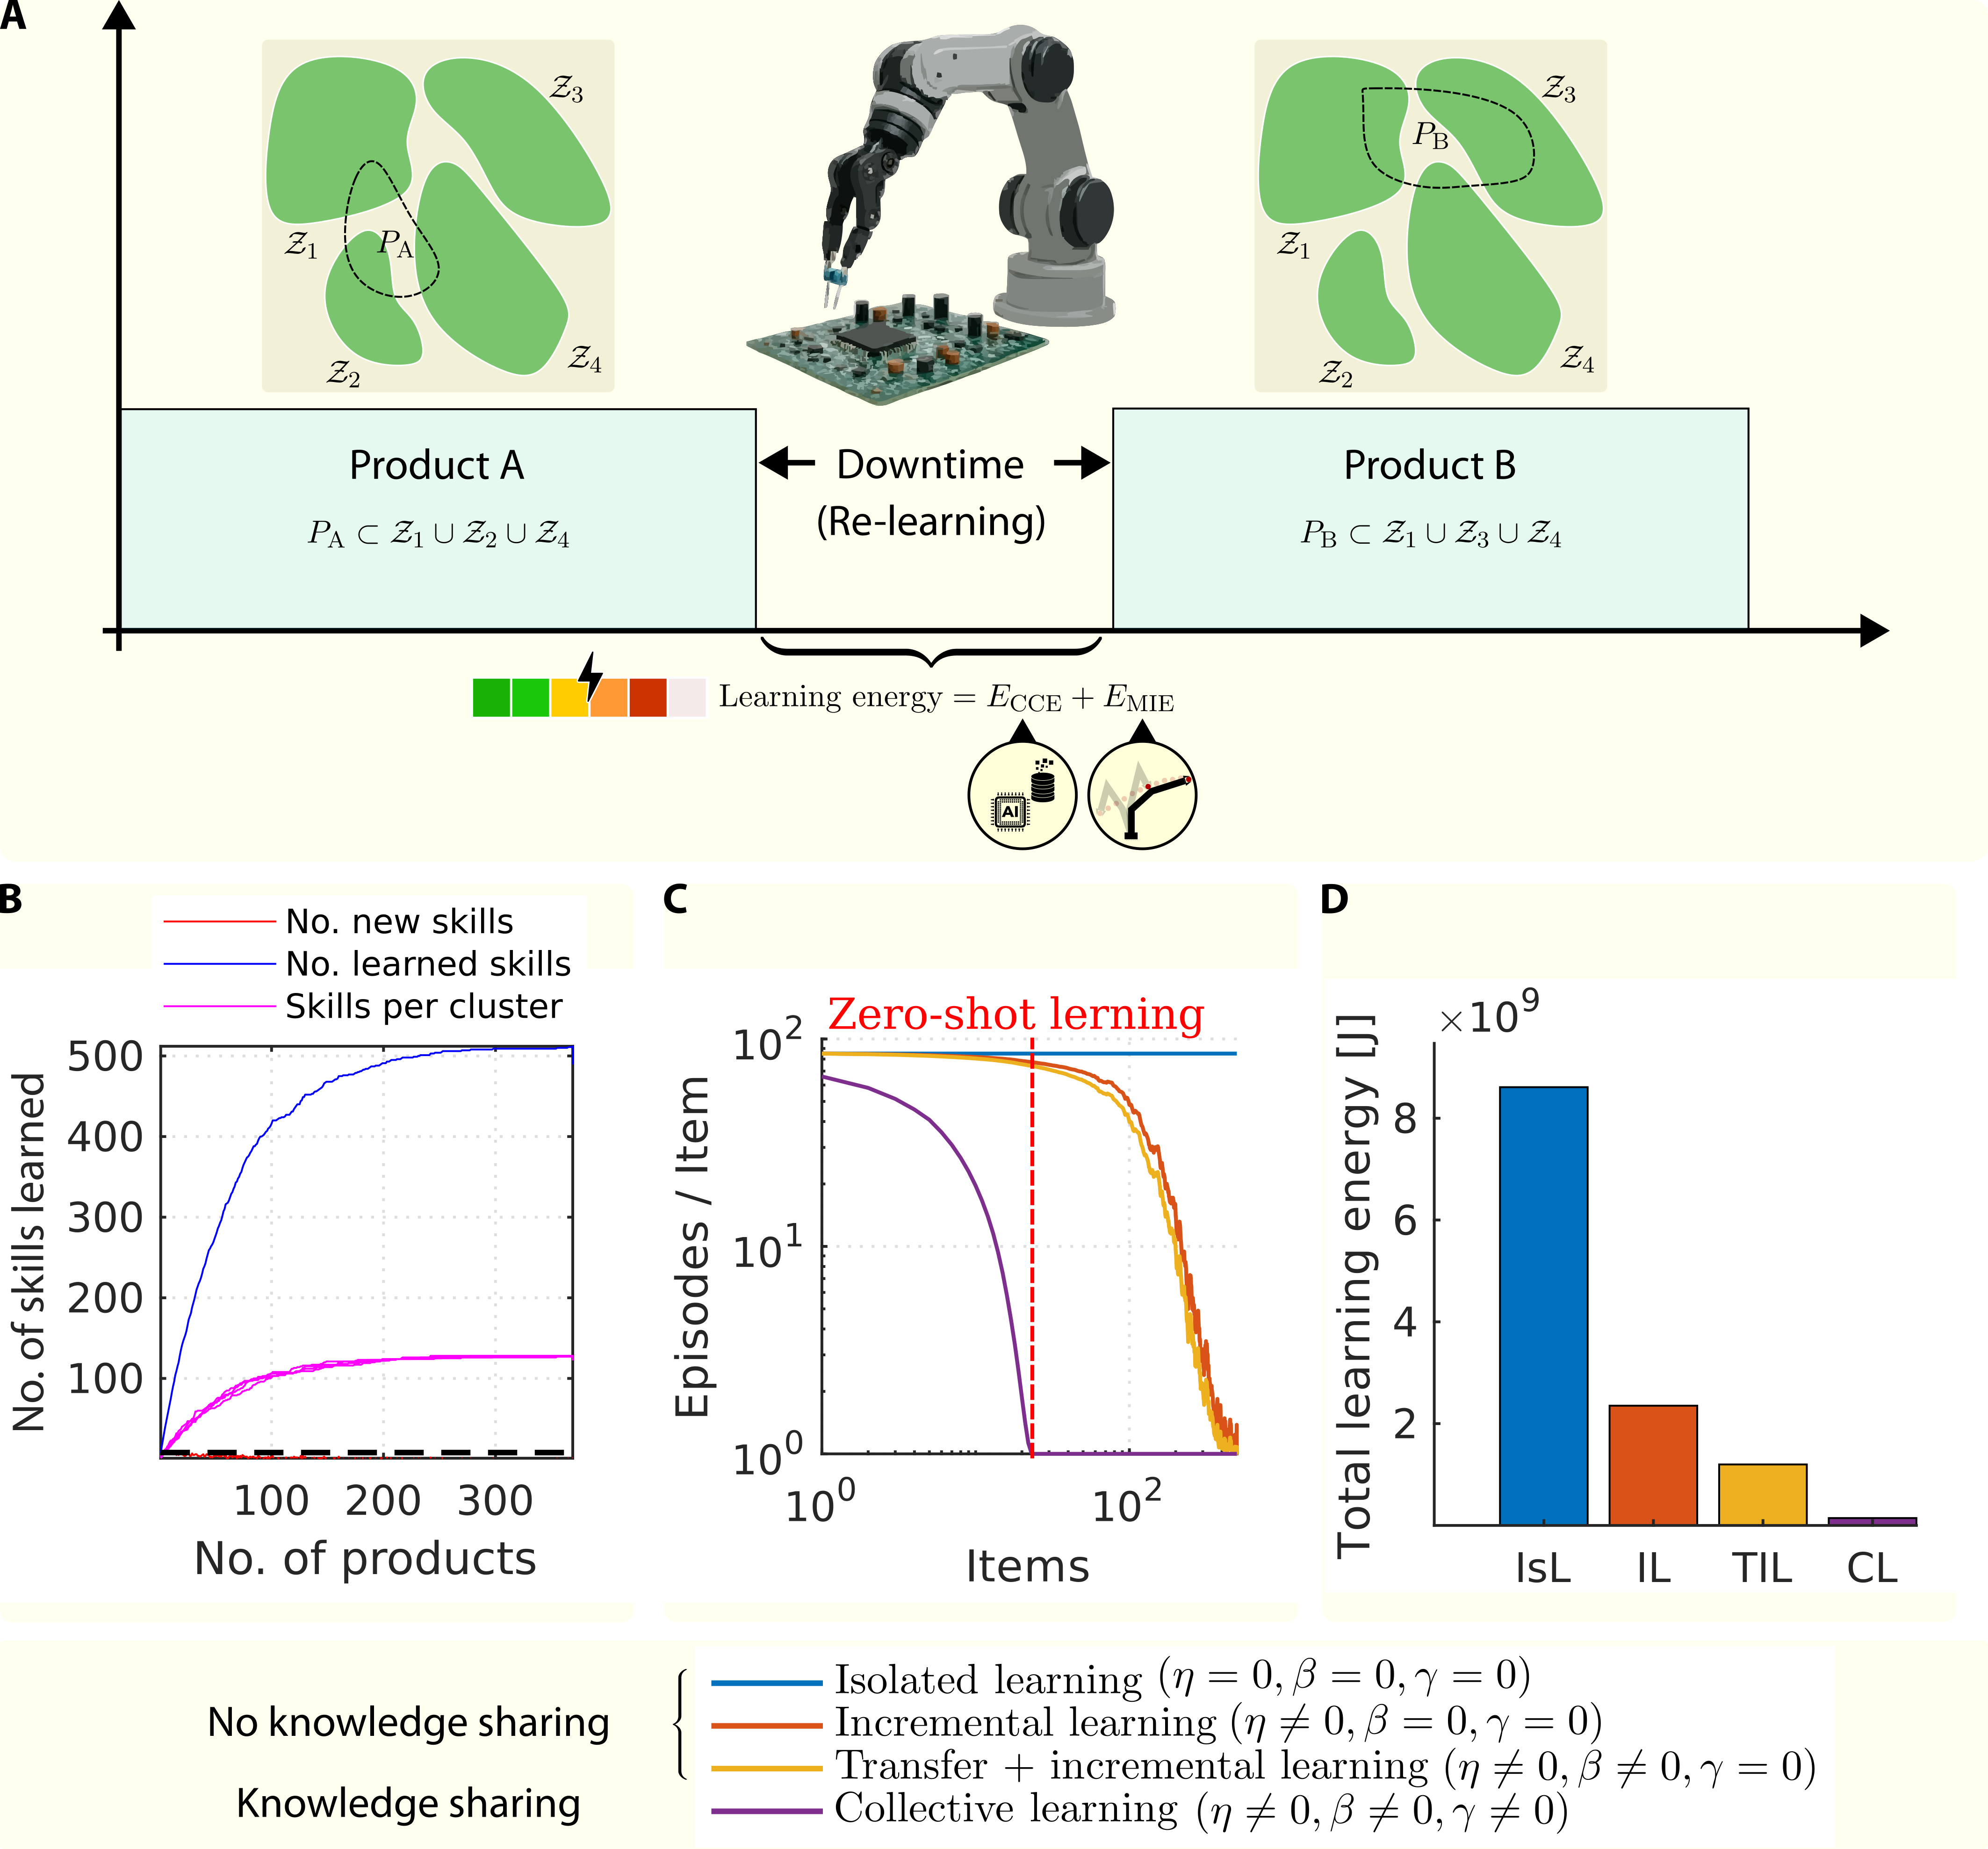
\includegraphics[width=16cm]{smart_factory_case_study.png}
	\hspace*{\fill}
	\caption[] {\label{fig:smart_factory_case_study} \textbf{Smart sensor manufacturing.} {(\textbf{A}) A factory manufactures a new smart sensor every shift. During downtime, a robot collective might need to learn a new set of skills to manufacture the new sensor. (\textbf{B}) The skills seen by the collective, according to the number of products, (\textbf{C}), the learning episodes required to learn a product, and (\textbf{D}), the total learning energy required to master all skills. %\TODO{Run more times to smooth the plot.}
    }}
\end{figure*}
% ---

In this second scenario, we run a case study of a smart factory setting where multiple robots learn different numbers of skills required for the manufacturing of a given product; in our case, advanced smart sensors. This use case emphasizes sample-efficient, real-world learning of manipulation skills to support flexible reconfiguration of work cells to manufacture different types of smart sensors. To resemble the conditions implied in Assumptions~\ref{assumption:average_behavior}, \ref{assumption:agent_similarity},~\ref{assumption:cluster_size}, and~\ref{assumption:cluster_transferability}, a prototypical skill learning scenario $\phi_\text{SF}$ for the smart  factory involves several robots performing multiple skills in different clusters. In this particular case, we settle for a smaller collective of $N_\mathrm{r} = 8$ robots and keep the values for the remaining elements of $ \bm{\rho} $ as in the previous scenario. 

%In practice, in our case study, we consider a smart factory environment dedicated to the rapid prototyping of advanced smart sensors. 
The smart factory is composed of flexible, reconfigurable work cells tailored to specific manufacturing processes (e.g., component placement, soldering, assembly, testing, and packaging), enabling rapid adaptation to new tasks and components. Within these cells, robots perform different skills, such as \textit{pick-and-place}, \textit{gripping and handling}, \textit{component orientation}, \textit{precise solder application}, \textit{optical inspection}, \textit{force testing}, \textit{printed-circuit-board handling}, and the like \cite{Kirschner2025CategorizingRB}. 

When a new sensor is required, that is, in changeover time, a new set of skills is required to manufacture the sensor. Under the assumption that hardware stays constant, this implies a production downtime period where the \ac{eai} agents need to learn these skills, see Fig.~\ref{fig:smart_factory_case_study}~\textbf{A}. For example, in one shift, the product $ P_\mathrm{A} $ is manufactured and requires robots to learn skills from three skill clusters ($ P_\text{A}\subset\mathcal{Z}_1
\cup\mathcal{Z}_2\cup\mathcal{Z}_4 $). At changeover time, now the skills needed to manufacture a new product $ P_\mathrm{B} $ are required ($P_\text{B}\subset\mathcal{Z}_1\cup\mathcal{Z}_3\cup\mathcal{Z}_4 $). For simplicity, we assume that every new product requires $ p $ skills and there may be repeated (already seen) skills in the skills of different products. Furthermore, we let $ N_\mathrm{r} \geq p $. The question in this scenario is to see whether \ac{cl} reduces the changeover downtime $ T_\mathrm{CO} $ to a minimum. In other words, it is desired to reduce the number of episodes required to learn the skills for a new sensor type to be manufactured. Using the conditions posed by the skill learning scenario $ \phi_\text{SF}$, we will show the advantages of using \ac{cl} on reducing the complexity of skill learning and thereby reducing downtime and energy consumption to learn the skills for all products.

The power-per-episode (see Asm.~\ref{assumption:power_and_episode_time}) is determined by the sum of the power required for basal processes, the power for motion and interaction, and the power for computation and communication, i.e.,
% ---
\begin{equation}
	P_0 = P_\text{BEE} + P_\text{MIE} + P_\text{CCE}.
\end{equation}
% ---
To assign a numerical value to $P_\text{BEE}$, and without loss of generality, we consider $\phi_\text{SF}$ an instance of a smart factory populated with state-of-the-art tactile robots~\cite{Kirschner2025CategorizingRB}, like those listed in Sec.~\ref{sec:app_cobot_ener_consumption} of the \nameref{sec:supplementary_materials}, which require a typical operational power of about $\unit[40]{W}$ (plus the compute power for basic functionalities). To approximate $P_\text{MIE}$, we estimate that in demanding tasks, the power requirement of a cobot and a tactile robot can be upper-bounded around $ \unit[300] {W} $. Finally, to determine $P_\text{CCE}$, we assume that, to deal with the computing effort that learning new skills will have on the robots' local processors, the smart factory will delegate the computational burden to a remote computing unit, i.e., cloud computing. Thus, we take as reference the work in \cite{Strubell2019EnergyPolicyConsiderations}, where a state-of-the-art machine learning algorithm executed in a cluster required $\unit[1.42]{kW}$ to solve a task. Finally, we can assume that the execution of each trial episode $n$ takes $\Delta t = 60$ seconds. Using these reference values, we can estimate that, when learning a skill, an average trial episode has an energetic demand of
% ---
%\begin{equation}
%	e_0 = P_0 \Delta t = \left(40 + 300 + 1,415.78\right) \left(60\right) \approx 105~\text{kJ}.
%\end{equation}
\begin{equation}
	e_0 = P_0 \Delta t \approx 105~\text{kJ}.
\end{equation}
% ---

Figure~\ref{fig:smart_factory_case_study}~\textbf{B} shows the learning progress in terms of the number of skills that have been seen as the number of products increases. Correspondingly, the number of episodes required to learn the batches of skills corresponding to different products is depicted in Fig.~\ref{fig:smart_factory_case_study}~\textbf{C}. It can be observed that, close to the 20 product mark, all other skills can be learned practically instantaneously (zero-shot learning). This means that the downtime associated with learning the skills for a product is negligible at this point. For comparison, similar plots for the conventional paradigms of \ac{isl}, \ac{il}, and \ac{til} are also provided (see \nameref{sec:methods} for more details). In these paradigms, there is no inter-agent knowledge exchange, which clearly impacts the number of learning episodes required. As expected, \ac{isl} exhibits the worst performance, always requiring $c_0$ episodes to learn every skill. \ac{il} shows improvement, but does not benefit from knowledge in other skill clusters. This is not the case in \ac{til}, as a robot can exploit the knowledge of the clusters it has visited. Finally, the speed of knowledge collection is exponentiated with \ac{cl}---reflected in the number of learning episodes---thanks to the exchange of knowledge among the $N_\mathrm{r}$ robots in the collective. Compared to the other learning paradigms, with \ac{cl}, a batch of skills (that is, a new product) is learned in a few episodes. This last fact is directly related to the energy required by the collective to learn all $N_\mathcal{S}$ skills. The bar plot in Fig.~\ref{fig:smart_factory_case_study}~\textbf{D} shows the energy required for each paradigm for all the learning episodes. \Acl{cl} uses only about 10~\% of the energy required by its closest competitor, \acl{til}.

% ===================================================================================================
%                                                 |                                                 |
%                                                 |                                                 |
% -------------------------------------------- SECTION ---------------------------------------------|
%                                                 |                                                 |
%                                                 |                                                 |
% ===================================================================================================
\section*{Discussion}\label{sec:discussion}

This work establishes a principled foundation for understanding and optimizing energy efficiency in \acl{eai} systems through the lens of \acl{cl}. We began by identifying three grand energy challenges posed by \ac{dai} and the growing population of robots: the escalating computational load, the increasing energy footprint of physical agents, and the manufacturing-related energy costs. We then introduced a formal framework for modeling energy expenditure in \ac{eai} agents and demonstrated that traditional learning paradigms---isolated, incremental, and transfer learning---fail to scale efficiently with system and skill universe size. In contrast, \acl{cl}, characterized by structured intra- and inter-agent knowledge exchange, emerged as a paradigm capable of accelerating learning and significantly reducing energy demands. Through analytical modeling and simulation studies, we revealed nine canonical \ac{cl} regimes and identified four principal behaviors---destructive, canceling, ideal, and compensating---that capture the interplay between individual and collective learning dynamics. Our results show that \ac{cl} can reduce energy consumption by at least an order of magnitude compared to conventional paradigms, especially in realistic smart factory settings. These findings highlight \ac{cl} as a scalable, fault-tolerant, and energy-efficient approach, offering a compelling path forward for sustainable AI and robotics.

% Despite the promise that \ac{cl} holds for energy efficient learning, some points remain

% ===================================================================================================
\begin{figure*}[t!]
	\centering
	\hspace*{\fill}
	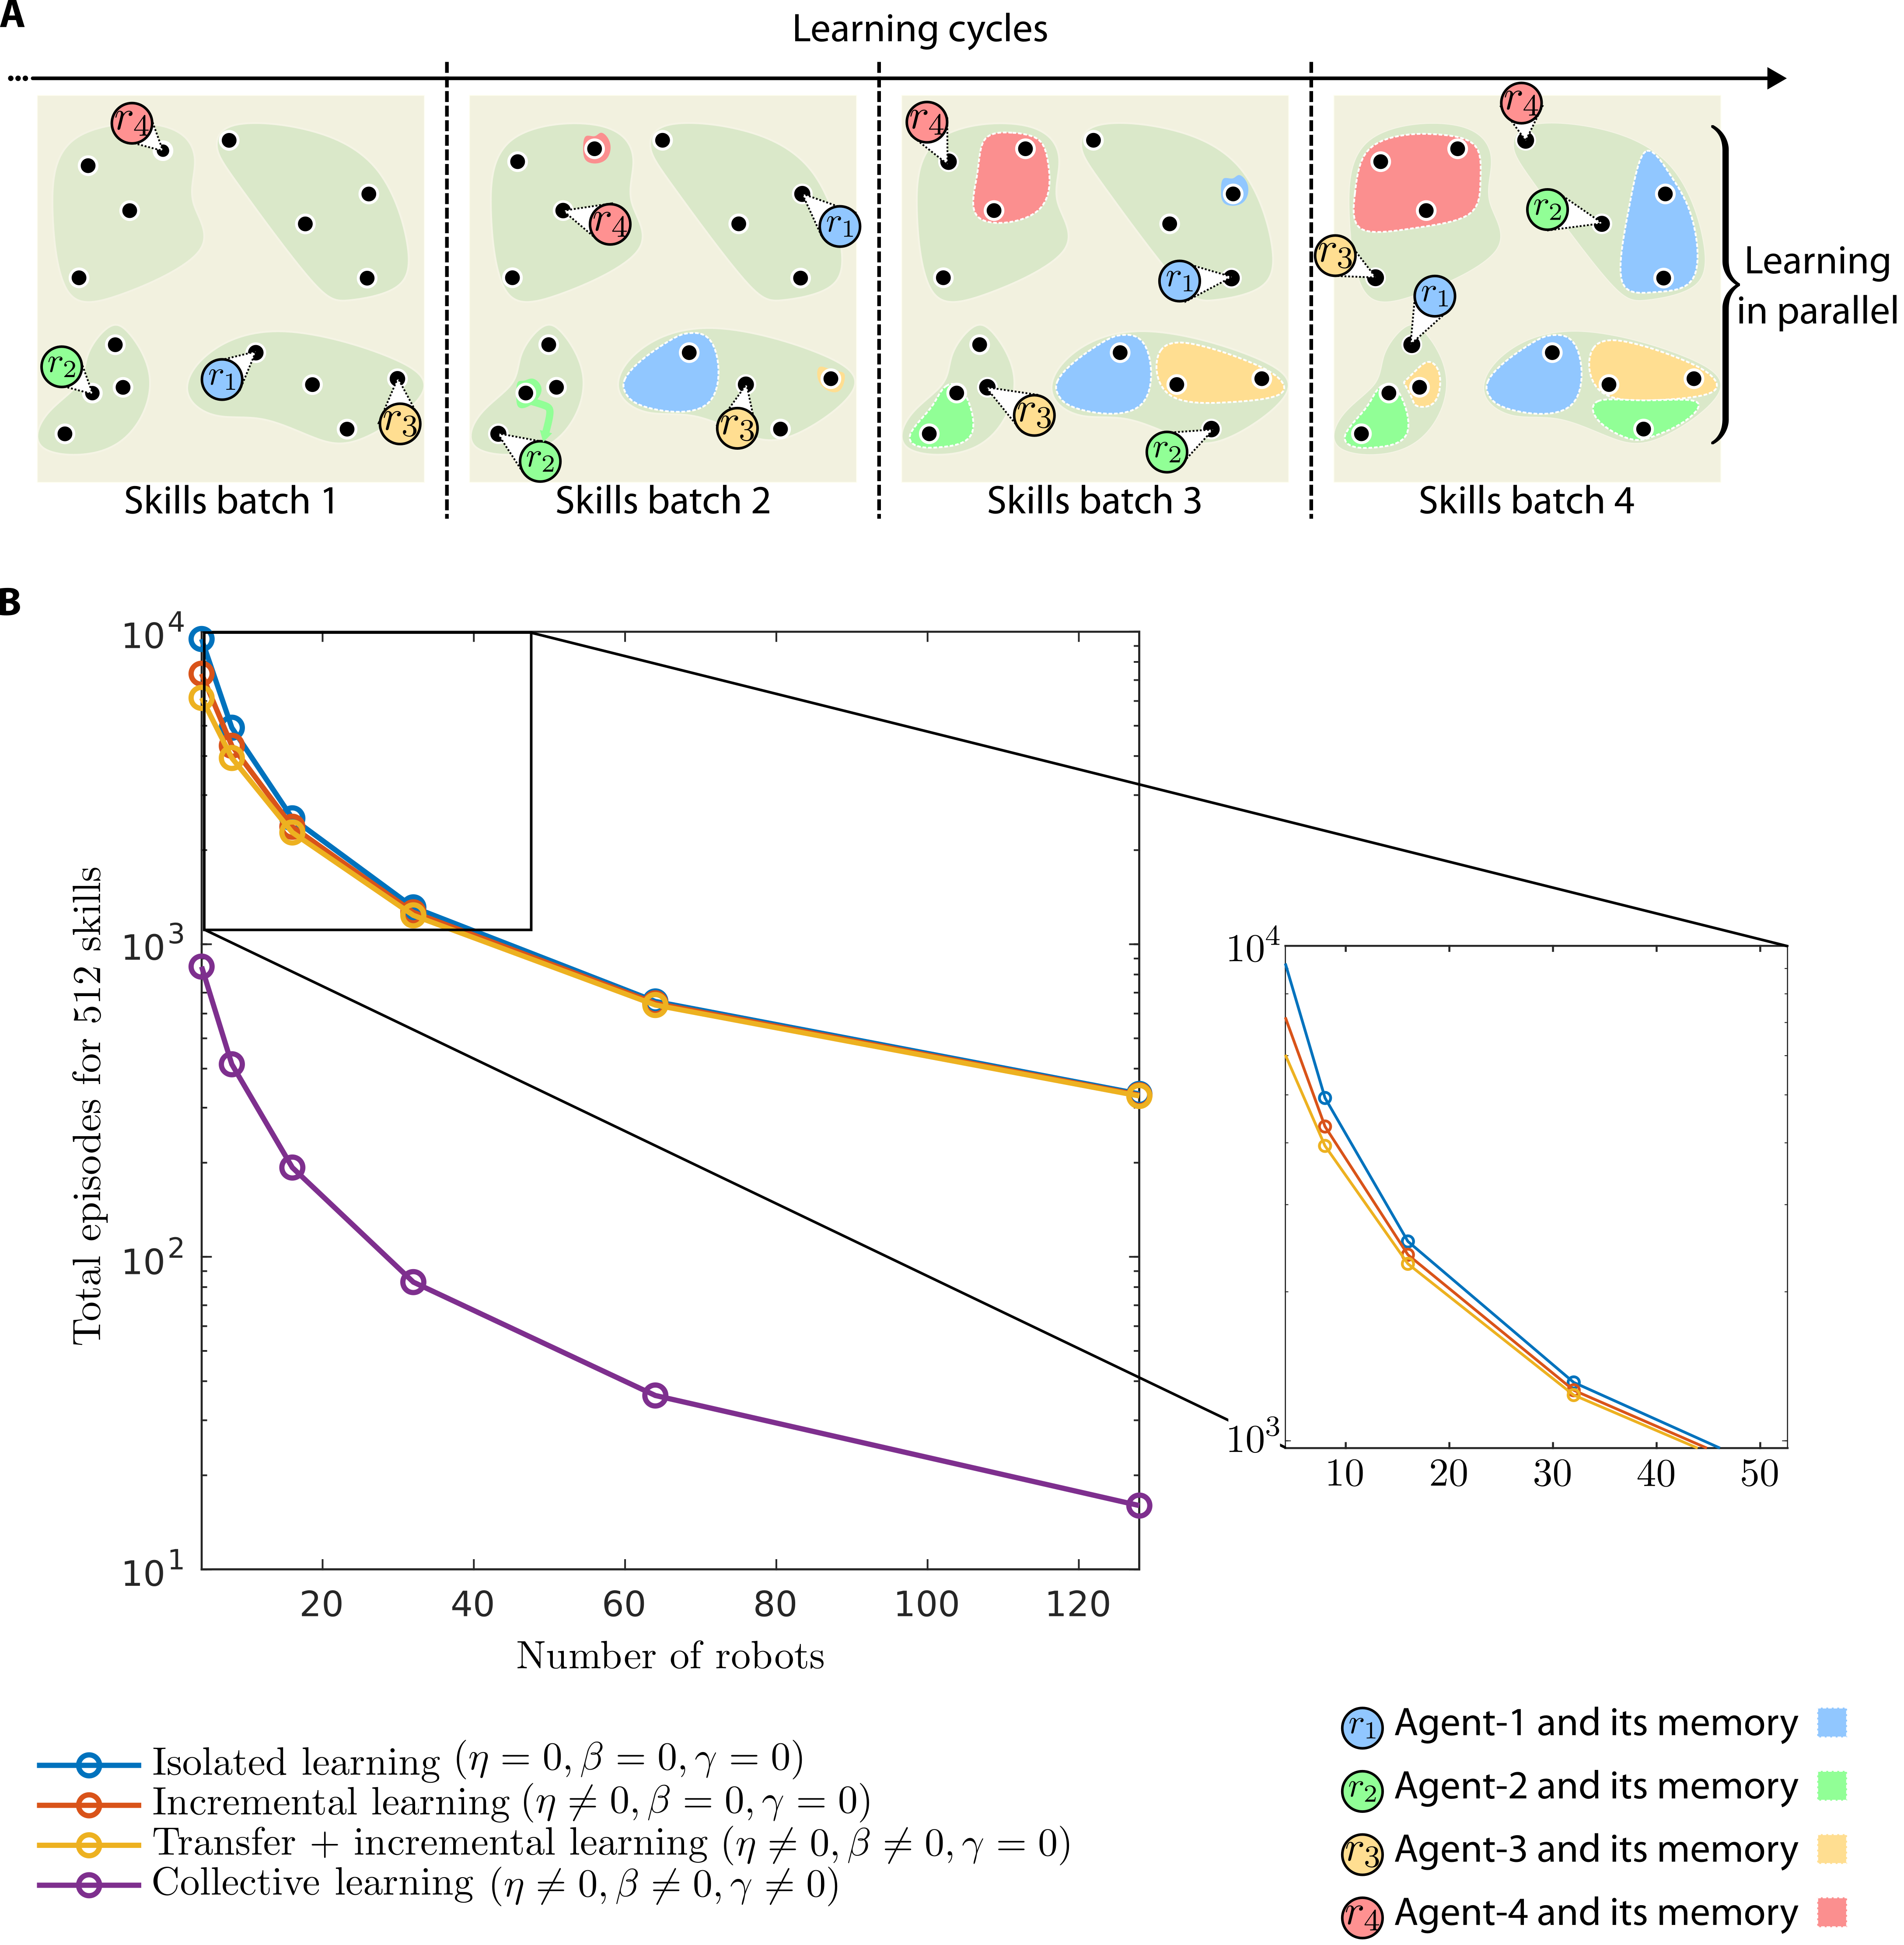
\includegraphics[width=16cm]{learning_paradigms_and_size_of_collective.png}
	\hspace*{\fill}
	\caption[] {\label{fig:learning_paradigms_and_size_of_collective} \textbf{Effect of the collective size on the total number of learning episodes.} {(\textbf{A}) In the classical paradigms, even when learning in parallel, each agent holds its own memory and can only access the subset of knowledge corresponding to the skills it has seen. This effectively splits the total knowledge. The more agents, the less available knowledge per agent. (\textbf{B}) The plot shows that as a result of having more agents, the classical paradigms degrade the learning and converge to \acl{isl}. On the contrary, \acl{cl} exploits the number of robots, exponentiating the learning as a result.}}
\end{figure*}
% ---

% ===================================================================================================
\paragraph*{Splitting knowledge vs. sharing knowledge}
% The performance plots in Fig.~\ref{fig:collective_learning_cases} showed different \ac{cl} regimes for a variying size of the collective. To assess how the number $N_\mathrm{r}$ of \ac{eai} agents and the number of skills learned $\kappa$ affects the total number of trial episodes $C_\mathcal{S}$ required to learn all the $N_\mathcal{S}$ skills in the different learning paradigms, we use the same parameters $\phi$ disucssed in as before but let the number of skills per batch be equal to the size of the collective.

The performance plots in Fig.~\ref{fig:collective_learning_cases} showed different \ac{cl} regimes for a varying size of the collective. It is also important to look at how the other discussed learning paradimgs behave based on the number $N_\mathrm{r}$ of \ac{eai} agents in the collective, which is directly related to the the total number of trial episodes $C_\mathcal{S}$ required to learn all the $N_\mathcal{S}$ skills, and, hence, to the learning energy expenditure via the constant $e_0$. The results of this analysis are shown in Fig.~\ref{fig:learning_paradigms_and_size_of_collective}. The first immediate implication of the lack of knowledge sharing among agents is that the total knowledge is effectively partitioned among the agents in the collective. This is conceptually illustrated in Fig.~\ref{fig:learning_paradigms_and_size_of_collective}~\textbf{A}, where four robots---identified in different colors for clarity---travel the skill manifold learning an equal number of skills in parallel. As the learning cycles progress, each agent holds in its memory a share of the total knowledge (depicted by the colored areas). It follows, that the more agents are in the collective, the more the total knowledge is partitioned among all the agents. This effect is shown in Fig.~\ref{fig:learning_paradigms_and_size_of_collective}~\textbf{B}, where it can be seen that, initially, \ac{il} is better than the trivial \ac{isl} case; however, as the collective size increases, the skill knowledge is divided among the available robots, which implies that less knowledge can be passed as the pool of learned skills $\zeta_k$ per robot decreases. This explains why the total number of trial episodes for \ac{isl} and \ac{il} approach each other in the limit. With a growing collective size, \ac{til} exhibits a similar behavior. Less cluster knowledge can be collected by each robot and transferred to a target cluster. With a larger collective, \ac{til} rapidly converges to \ac{il} and eventually to \ac{isl}. Unlike these conventional paradigms, in \ac{cl}, as the size of the collective robots grows, the total complexity keeps decreasing as a result of the knowledge exchange from all the robots learning skills from different clusters at the same time.

% ===================================================================================================
\paragraph*{On the regimes of \acl{cl} systems}
% Various factors can influence the dynamics that govern a \ac{cl} system, including embodiment, false communication, communication breaches, updates to the learning rate, and the correctness of the information transferred. Each of these factors can alter the key parameters of the model, namely $\alpha$, $\eta$, and $\gamma)$, thereby affecting the overall behavior of the system. Although the effects of embodiment distribution are primarily addressed by Assumptions~\ref{assumption:average_behavior} and \ref{assumption:agent_similarity}---see \nameref{sec:methods}. Recall that the parameters, $\alpha_i$, account for how efficiently the agents are in learning a skill, mostly related to their embodiment. Yet, $\alpha_i$ does not hinder the learning, only makes it faster or slower. Strongly linked to the skill similarity within a cluster, but ultimately reflected on the agent's capacity to use the already acquired knowledge, variations in $eta_i$ can actually thwart the learning.  Despite these variations, the idealized collective effect persists, provided that the inter-agent exchange factor $\gamma$ is chosen sensibly to maintain the stability of the system. Indeed, one of the most important and intriguing findings is the identification of regimes in which \ac{cl} significantly  any conventional learning paradigms. Remarkably, this advantageous regime aligns with parameter ranges that are likely to arise in real-world scenarios, underscoring the relevance and promise of the collective knowledge-sharing paradigm.


% Various factors can influence the dynamics that govern a \ac{cl} system, including differences in embodiment, communication errors, breaches in information exchange, updates to the learning rate, and the correctness of the information being transferred. Each of these factors can affect the key parameters of the model---namely, $\alpha$, $\eta$, and $\gamma$---thereby shaping the overall behavior of the system. The impact of embodiment distribution is addressed primarily by Assumptions~\ref{assumption:average_behavior} and \ref{assumption:agent_similarity} (see \nameref{sec:methods}). The parameter $\alpha_i$ captures how efficiently an agent can learn a skill, primarily reflecting its embodiment. Although differences in $\alpha$ influence the speed of learning, they do not prevent it from occurring. In contrast, $\eta$---which is closely related to skill similarity within a cluster and reflects an agent’s ability to reuse previously acquired knowledge---can directly hinder learning when its value is too low. Despite these potential variations, the \acl{cl} effect remains robust, provided that the inter-agent exchange factor $\gamma$ is chosen appropriately to ensure system stability; recall $\gamma$ accounts for the stable and efficient communication. Based on the values of these parameters, one of the most significant findings is the emergence of regimes in which \ac{cl} substantially outperforms conventional learning paradigms. In particular, these beneficial regimes correspond to parameter ranges that are likely to occur in real-world systems, reinforcing the practical relevance and promise of collective knowledge sharing.


The dynamics of a \ac{cl} system are shaped by multiple interacting factors, including differences in embodiment, inaccuracies in communication, breaches in synchronization, updates to learning parameters, and the correctness of the information exchanged. These factors manifest through variations in the key model parameters: the agents learning rates $\bm{\alpha}$, the intra-agent retention gains $\bm{\eta}$, and the inter-agent exchange gains in the matrix $\bm{\Gamma}$. As discussed in \nameref{sec:methods}, Assumptions~\ref{assumption:average_behavior} and~\ref{assumption:agent_similarity} constrain embodiment heterogeneity, which primarily influences $\alpha$, the rate at which an agent acquires new skills in isolation. While the individual entries in $\bm{\alpha}$ affect the speed of learning, it does not qualitatively change whether learning succeeds or fails. In contrast, $\bm{\eta}$ reflects an agent’s ability to reuse and reinforce previously acquired knowledge. Since it is sensitive to the similarity structure of skills within a cluster, low vaues in $\bm{\eta}$ can actively hinder the learning process, even in otherwise competent agents. Nevertheless, the system-level behavior remains robust if the average values of the entries in the inter-agent transfer matrix $\bm{\Gamma}$ are chosen appropriately to maintain the stability of knowledge sharing across the collective. One of the most compelling findings is the existence of regimes in which \ac{cl} outperforms conventional, isolated learning paradigms. These regimes---particularly the ideal and compensating ones---emerge within realistic parameter ranges and demonstrate how even weak or noisy agents can succeed collectively through effective knowledge integrations and sharing. This highlights the practical relevance and potential of \ac{cl} systems as scalable, fault-tolerant architectures for distributed intelligence.

% ===================================================================================================
% ---
\begin{figure}[!th]
	\centering
	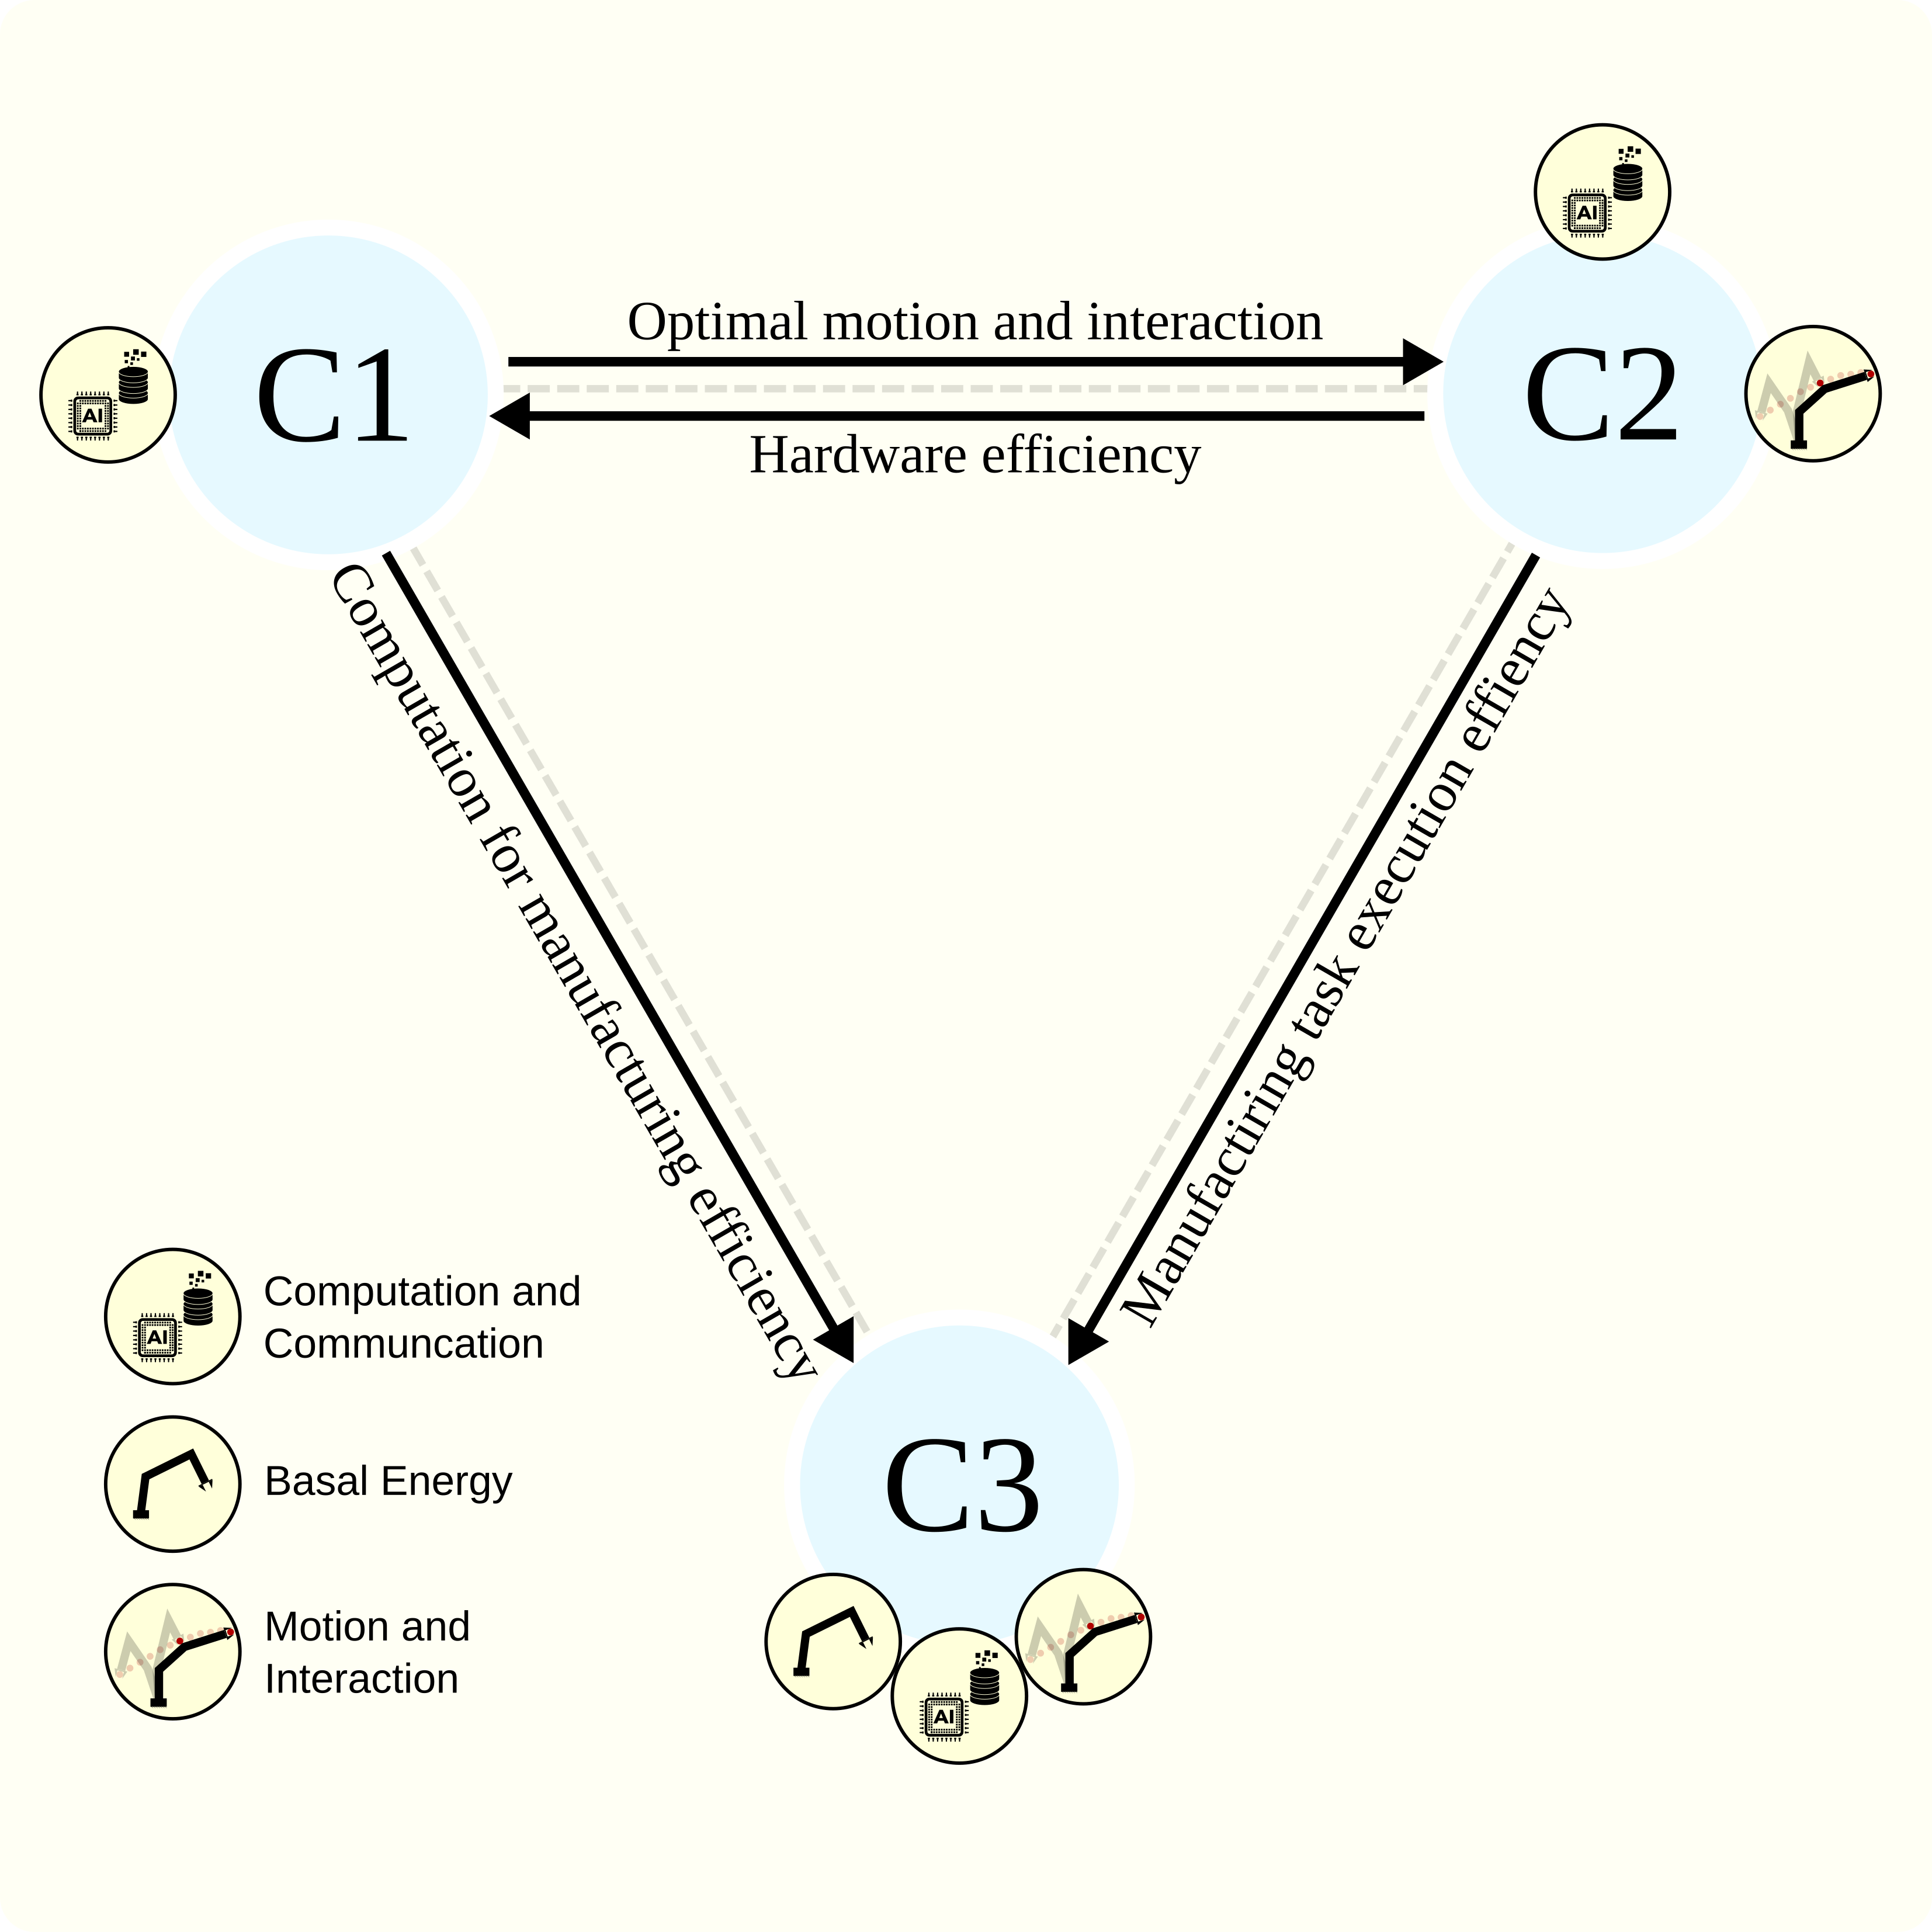
\includegraphics[width=0.45\textwidth]{fig/grand_challenges_connections.png}
	\caption{\textbf{Interconnection between energy challenges C1, C2, and C3.}}
	\label{fig:challengesConnected}
\end{figure}
% ---


% ===================================================================================================
\paragraph*{Developing collective learning to address the energy challenges of \acl{eai}}

\Acl{cl} directly speaks to each of the three grand energy challenges introduced earlier. The natural connections between these challenges---shown in Fig.~\ref{fig:challengesConnected}---and their association with \ac{eai} allow us to identify critical areas of opportunity for \ac{cl}.
\newline
(C1) Computation and communication energy ($E_\text{CCE}$).
In current practice, every robot or \ac{ai} system repeatedly computes policies or retrains models in isolation. This multiplies the demand for GPU clusters and cloud resources. By contrast, \ac{cl} allows skills acquired by one agent to be stored, exchanged, and reused by others. Instead of thousands of redundant training runs across agents, the collective can converge after a few representative experiences, with subsequent agents retrieving stored knowledge. Over time, this shifts the resource profile from expensive parallel training toward lighter operations such as querying and incremental updates, which drastically reduces GPU hours and associated data center energy.
\newline
(C2) Energy footprint of physical robots ($E_\text{BEE}$ and $E_\text{MIE}$).
Physical learning is costly: each trial requires actuation, sensing, and interaction with the environment. In conventional paradigms, multiple robots would each practice the same task, consuming energy in proportion to the collective size. In principle, with \ac{cl}, only a subset of robots needs to explore a skill physically; others can learn from their experience through structured knowledge transfer. This shortens the number of required trials per agent, lowers total motion and interaction energy, and reduces downtime in settings like smart factories where production stops during learning phases. In other words, \ac{cl} minimizes how often robots must ``burn electricity to move'' in order to master skills.
\newline
(C3) Manufacturing-related energy.
The energy demand associated with producing more and more robotic and computational hardware grows with the size of the collective. \ac{cl} indirectly addresses this challenge by enabling better use of existing robots. If robots learn faster and more efficiently through knowledge sharing, fewer redundant units are required to maintain productivity, and existing fleets can adapt to new tasks without costly hardware replacement. Furthermore, by reducing retraining loads and unnecessary trial-and-error wear, \ac{cl} can extend the service life of robots and electronic components, thereby lowering the frequency of new production cycles and amplifying the benefits of recycling strategies.
\newline
Taken together, these links show that \ac{cl} is not just a conceptual advance but a practical lever for reducing energy demand across all layers of embodied \ac{ai}---from cloud computation, to real-world robot trials, to manufacturing pipelines.

% ===================================================================================================
\paragraph*{Reinterpreting Incremental and Transfer Learning in the Age of Foundation Models}

\myhl{To situate our framework within the broader landscape of machine learning, we revisit the notions of incremental and transfer learning in light of recent advances in large-scale foundation models. Our interpretation of \ac{il} and \ac{tl} differs from the conventional acceptations in the machine learning community. \Ac{il} is typically defined as the sequential update of model parameters to prevent forgetting, while \ac{tl} refers to reusing pre-trained knowledge across domains through fine-tuning. In our framework, however, these notions are defined structurally: \ac{il} corresponds to \emph{intra-cluster reuse}, where knowledge acquisition rates scale with the number of learned skills, and \ac{tl} corresponds to \emph{inter-cluster reuse}, governed by transferable fractions and the similarity matrix~$\bm{B}$. A comparative summary of these distinctions is provided in Table~\ref{tab:IL_TL}.}

\myhl{By contrast, recent advances in large language, vision--language(-action), and other foundation models are often framed as exhibiting \ac{il} or \ac{tl}, since pre-trained generalist policies can later be fine-tuned for specific tasks. Yet their underlying mechanisms differ fundamentally from the idealized learning paradigms as considered in our work. Foundation models are trained on vast data sets---such as natural language, multimodal, or cross-embodiment corpora---and adapted via prompting, fine-tuning, or retrieval-augmented generation (RAG). This process does not constitute genuine \ac{il} within a domain, nor structured \ac{tl} across domains. Instead, it reflects large-scale statistical pattern matching: correlations extracted in one representational universe are repurposed in another, without explicit exploitation of transferable skill knowledge. Within the context of skill learning, the information encoded in a foundation model may offer only a coarse approximation of a skill, obtained without embodied interaction and therefore bypassing the \ac{slad} challenge.}

\myhl{\textbf{The idealized knowledge dynamics described by Eq.~\eqref{eq:collective_knowledge_dynamics} capture the continuous integration of knowledge bits from all \ac{eai} agents. In contrast, foundation models undergo a one-time global training (learning) phase followed by static inference. Their inference stage bears a superficial resemblance to \ac{tl}, as pre-trained knowledge is reused across tasks; yet inference can be seen as effectively providing only an initial condition for the knowledge integrator. Even when combined with RAG, such systems remain incapable of genuine \ac{il}, as they cannot incorporate new knowledge dynamically through interaction. Recent efforts to fuse foundation models with reinforcement learning~\cite{firoozi2025foundation} attempt to complement this limitation with reinforcement learning viewed as a specific form of \ac{il}, where experience incrementally refines a policy under a reward function.}}

\myhl{While explicit skill similarity is not exploited in foundation models, limited forms of transfer may occur between ``skill universes'' that share comparable similarity structures, where only the domain-specific data layer changes. In such cases, skills that appear transferable across representational universes do not arise from genuine knowledge integration or discovery. Beyond this epistemic limitation lies an energetic one: foundation models externalize learning into massive, centralized pretraining cycles, whereas \ac{cl} distributes it across many embodied agents that generate, exchange, and refine knowledge in real time. This transition from statistical accumulation to distributed embodiment points toward a more scalable and energetically sustainable paradigm for \ac{eai}.}
% \paragraph*{Reinterpreting Incremental and Transfer Learning in the Age of Foundation Models}
% \myhl{To situate our framework within the broader landscape of machine learning, we revisit the notions of incremental and transfer learning in light of recent developments in large-scale foundation models. Our definitions differ from the conventional usage in the machine learning community. \Ac{il} is typically understood as the sequential update of model parameters to prevent forgetting, while \ac{tl} refers to reusing pre-trained knowledge across domains through fine-tuning. In our framework, however, these notions are defined structurally: \ac{il} corresponds to \emph{intra-cluster reuse}, where knowledge acquisition rates scale with the number of learned skills, and \ac{tl} corresponds to \emph{inter-cluster reuse}, governed by transferable fractions and the similarity matrix~$\bm{B}$. A comparative summary of these distinctions is provided in Table~\ref{tab:IL_TL}. As an analogy, reinforcement learning can be seen as a particular instance of \ac{il}, where new experiences incrementally refine a policy under a specific reward function.}

% \myhl{By contrast, recent advances in large language, vision-language(-action), and other foundation models are sometimes framed as exhibiting \ac{il} or \ac{tl}, since pre-trained generalist policies can later be fine-tuned for specific tasks. Yet their underlying mechanisms differ fundamentally from the learning paradigms considered here. Foundation models are trained on vast data sets---such as natural language, multimodal, or cross-embodiment corpora---and adapted via prompting, fine-tuning, or retrieval-augmented extensions. This process does not constitute genuine \ac{il} within a domain, nor structured \ac{tl} across domains. Instead, it reflects large-scale statistical pattern matching: correlations extracted in one representational universe are repurposed in another, without explicit exploitation of transferable skill knowledge. Within the context of skill learning, the information encoded in a foundation model may offer only a coarse approximation of a skill. Such approximations are not obtained through embodied learning but through a process that effectively circumvents the \ac{slad} challenge by relying on pre-existing data rather than real-world interaction.}

% \myhl{While explicit skill similarity is not exploited in foundation models, limited forms of transfer may occur between ``skill universes'' that share comparable similarity structures, where only the domain-specific data layer changes. In such cases, skills that appear transferable across representational universes do not result from genuine knowledge integration or discovery. Beyond this difference lies an energetic one: foundation models externalize learning into massive, centralized pretraining cycles, whereas \ac{cl} distributes it across many embodied agents that generate, exchange, and refine knowledge in real time. This transition from statistical accumulation to distributed embodiment points toward a more scalable and energetically sustainable paradigm for \ac{eai}.}

% ===================================================================================================
\paragraph*{Closing remarks}
Although unprecedented strides in \ac{ai} and robotics have revolutionized numerous sectors, the ongoing proliferation and associated energy escalation cannot be ignored. As the scope of \ac{ai} continues to expand, a concerted effort is required to strike a balance between innovation and conscientious use of energy to steer \ac{ai} toward sustainable operation.

To emphasize the importance of energy demands in \ac{ai} systems, we discussed three principal categories of energy expenditure and contrasted them with the great challenges posed by the increase in \acl{dai} applications and the growing population of \ac{eai} agents. In particular, we underscored that mitigating energy consumption in \ac{eai} systems requires not only improved mechanical designs and efficient computational and communication hardware, but also a paradigm shift toward sharing, exchange, transfer, and accumulation of knowledge acquired by individual agents.

As discussed in \cite{Kaelbling2020foundationefficientrobot}, efficient robotic learning algorithms must exhibit several key attributes to enable agents to acquire new skills on the fly: sample efficiency, generalizability, compositionality, and incremental learning capabilities. The \acl{cl} paradigm inherently fulfills these requirements by leveraging the full communication potential of networked \ac{eai} agents. This approach supports real-time, concurrent knowledge exchange and aggregation, yielding both energy- and time-efficient skill acquisition.

Our results show that relying on conventional paradigms--such as isolated, incremental, or transfer learning, as is also the case for foundation models---for large numbers of \ac{eai} agents leads to suboptimal energy utilization. Even when agents operate concurrently, the absence of genuine inter-agent knowledge exchange causes energy demands to scale inefficiently with agent population size. In contrast, our simulation study shows that \ac{cl} provides a compelling solution, especially when skill similarity guides the exchange process. In particular, the \ac{cl} paradigm achieved vastly improved performance as the number of robots increased, enabling concurrent learning of multiple skills with improved energy efficiency.

Although the promise of \ac{cl} is clear, it is important to acknowledge that the foundational algorithms and infrastructure required to realize this paradigm are either still in development or yet to be established. Even state-of-the-art approaches to incremental and transfer learning (e.g., reinforcement learning, vision-language-action models, and foundation models) remain in the early stages. However, although our main focus has been on the energy efficiency of the \ac{eai} systems, the implications of \ac{cl} extend well beyond this domain.

The \ac{cl} paradigm is equally relevant to \ac{dai} agents. Recent advances in edge computing and federated learning illustrate this potential, as they shift computational tasks from centralized data centers to the periphery, where \ac{dai} agents operate. Additionally, foundation models--trained through extensive learning efforts---are increasingly being reused and fine-tuned to solve more specific, nuanced tasks, demonstrating the value of effective knowledge transfer.

As in \ac{eai}, the advantages of \ac{cl} for \ac{dai} become evident when efficient mechanisms for knowledge exchange and aggregation are established among agents who execute their own learning routines. The synergies enabled by this paradigm can significantly increase both problem-solving capacity and energy efficiency in a wide range of \ac{dai} applications.

In conclusion, the \acl{cl} approach holds the potential to address key challenges at the intersection of energy efficiency, scalability, and adaptability in both embodied and distributed \ac{ai}. Our arguments and results can catalyze further research and development efforts, ultimately advancing the realization of collective learning across the entire spectrum of the \ac{ai} domains.

% ===================================================================================================
%                                                 |                                                 |
%                                                 |                                                 |
% -------------------------------------------- SECTION ---------------------------------------------|
%                                                 |                                                 |
%                                                 |                                                 |
% ===================================================================================================
\section*{Methods}\label{sec:methods}

% ===================================================================================================
\paragraph*{Modeling skill knowledge acquisition dynamics}\label{sec:knowledge_dynamics_model}
Understanding the energy and time demands represented by a team of $N_\mathrm{r}$ robots learning a skill universe $\mathcal{S}=\left\lbrace s_1,s_2,\ldots s_j,\ldots, s_{N_\mathcal{S}}\right\rbrace$, with $|\mathcal{S}| = N_\mathcal{S}$, requires analizing how skill knowledge is gained and what effect it may have on the acquisition of any new skill knowledge. 

To start, we refer to the \emph{complexity} $c_j$ of skill $ s_j $ as the number of trial episodes $n$ required to successfully learn it, namely, all actions and states visited by an \ac{eai} agent until a predefined stopping criterion is reached. Additionally,
% ---
\begin{tcolorbox}
	\begin{assumption}\label{assumption:power_and_episode_time}
		the average behavior of a system where both $N_\mathrm{r}$ and $N_\mathcal{S}$ are large can be described by the power $P_0$ required by any agent during learning and the mean execution time $\Delta t$ of every trial episode $n$, with both approximately constant; see Fig.~\ref{fig:power_per_episode}.
	\end{assumption}
\end{tcolorbox}
% ---
\noindent As a consequence of Asm.~\ref{assumption:power_and_episode_time}, and according to Eqs.~\eqref{eq:energy_per_episode},\eqref{eq:energy_per_skill}, and \eqref{eq:total_energy} in Sec.~\ref{sec:energy_time_and_power_per_episode}, the energy demand of an \ac{eai} agent learning a skill (or set of skills) is in first-order directly proportional to the skill(s) complexity.

% ===================================================================================================
%\paragraph*{Similarity and knowledge}
Let $\mathcal{Z}_k \subset \mathcal{S}$ be a subset of $N_{\mathcal{Z}_k}$ highly similar skills; that is, a \emph{cluster} of similar skills, see Fig.~\ref{fig:collective_learning_and_skill_manifold_conceptualization}~\textbf{A} and  Fig.~\ref{fig:skill_similarity_and_knowledge}~\textbf{A}. Furthermore, consider a second set $\mathcal{\zeta}_k \subset \mathcal{Z}_k$ that denotes the skills from $\mathcal{Z}_k$ that a given agent $i$ has already learned. Furthermore,  
%---
\begin{tcolorbox}
	\begin{assumption}\label{assumption:skill_clustering} the effect of a significant similarity among a set of skills is characterized by the acceleration of the overall learning process due to exchange of acquired knowledge from these skills.
	\end{assumption}
\end{tcolorbox}
% ---
% \noindent This implies that the $j$-th skill in the $k$-th cluster $s_{j,k} \in \mathcal{Z}_k$ can always benefit from the knowledge contained in $\mathcal{\zeta}_k$. Consequently, the more skills in $\mathcal{\zeta}_k$, the less knowledge about $ s_{j,k} $ remains to be learned. To model this effect, we introduce the remaining knowledge function $\bar{\sigma}_{j,k}\left(n\right)\in [0,1]$ expressing the knowledge about a skill $s_{j,k} \in \mathcal{Z}_k \setminus \mathcal{\zeta}_k$ that \emph{is not} contained in the knowledge base of $\mathcal{\zeta}_k$. The function $\bar{\sigma}_{j,k}(\cdot)$ satisfies
\noindent This implies that if $s_{j} \in \mathcal{Z}_k$, then agent $i$ can improve the learning of the skill benefiting from the knowledge contained in $\mathcal{\zeta}_k$. Consequently, the more skills in $\mathcal{\zeta}_k$, the less knowledge about $ s_{j} $ remains to be learned. To model this effect, we introduce the to-be-learned knowledge function $\bar{\sigma}_{i,j}\left(n\right)\in [0,1]$ expressing the knowledge about a skill $s_{j} \in \mathcal{Z}_k \setminus \mathcal{\zeta}_k$ that \emph{is not yet} contained in the knowledge base $\mathcal{\zeta}_k$. The function $\bar{\sigma}_{i,j}(\cdot)$ satisfies
% ---
\begin{equation}\label{eq:sigma_bar_conditions}
	\bar{\sigma}_{i,j}\left(n\right) = 
	\begin{cases}
		1 & \text{$\mathcal{\zeta}_k=\emptyset$},\\
		0 &\text{$\mathcal{\zeta}_k$ has \emph{all} knowledge of $s_{j}$}.
	\end{cases}
\end{equation}
% ---
Conceptually, $\bar{\sigma}_ {i,j}\left(\cdot\right)$ is the fraction of knowledge from ${\mathcal{Z}_k}$ that remains to be learned.
% ---
%\begin{figure*}[!t]
%	\centering
%	\hspace*{\fill}
%	\begin{subfigure}[t]{7.5cm}
%		\subcaption{}
%		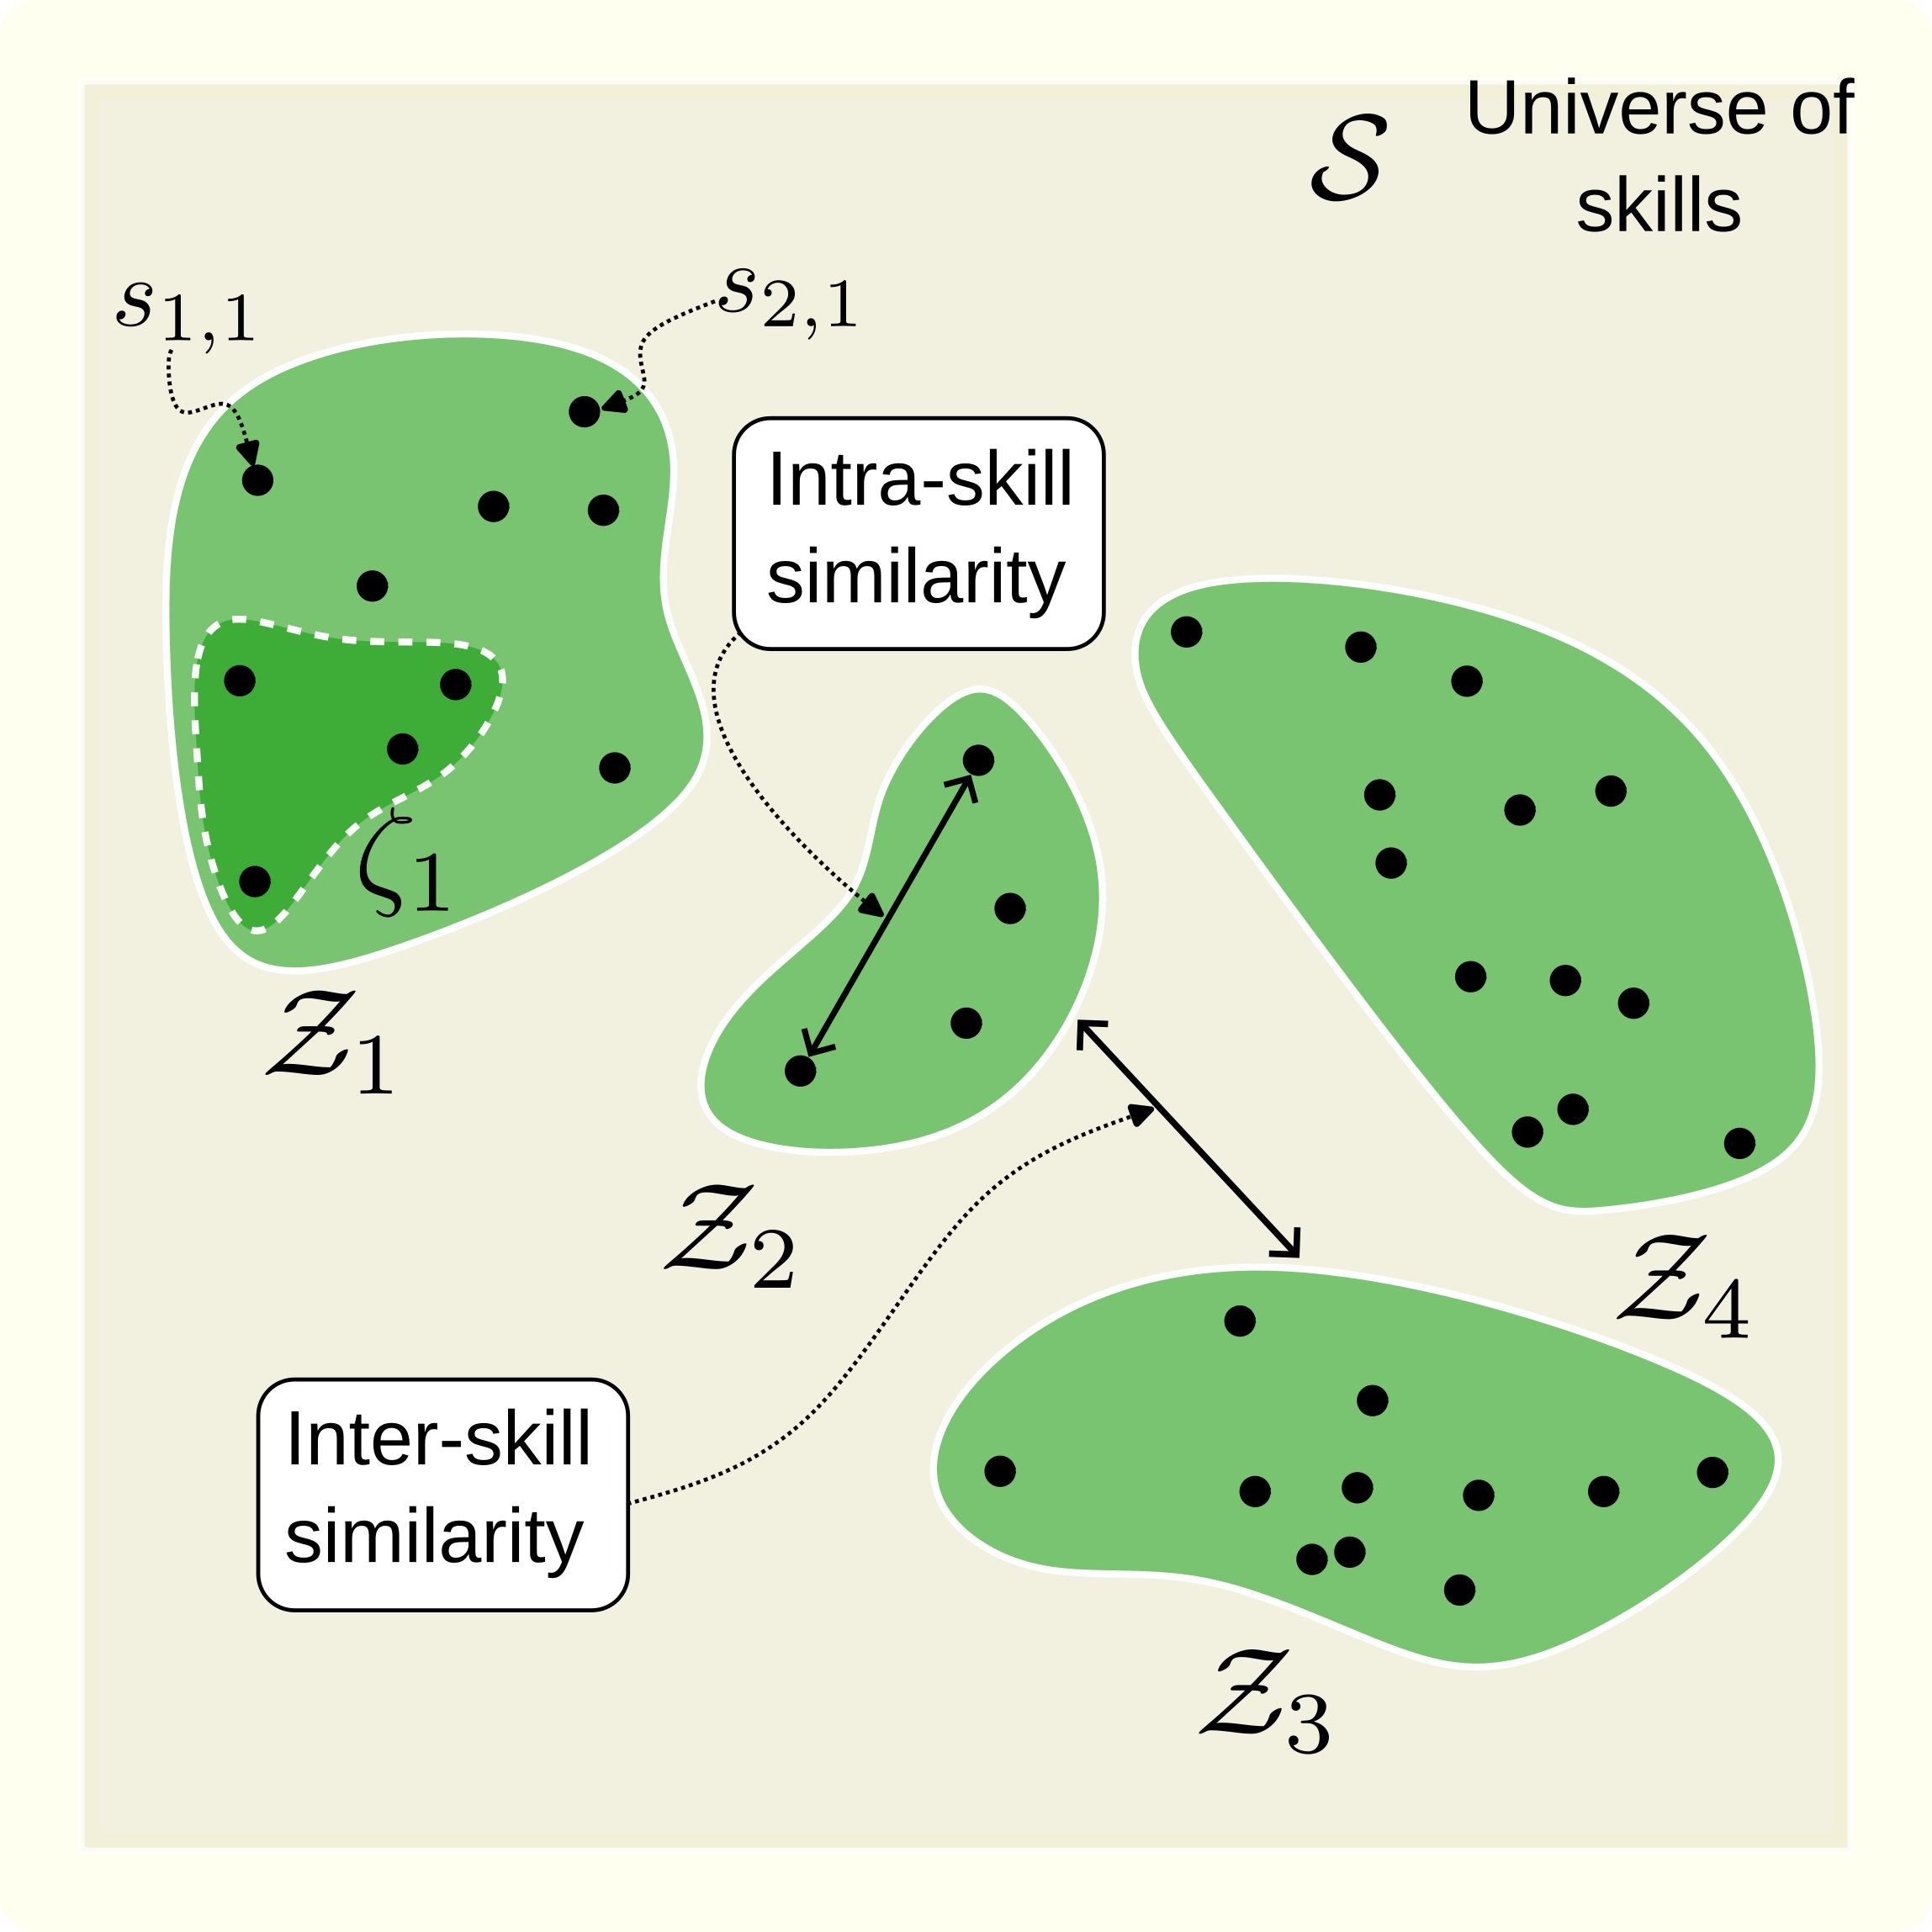
\includegraphics[width=\textwidth]{skill_similarity.png} \label{fig:skill_similarity}
%	\end{subfigure}
%	\hfill
%	\begin{subfigure}[t]{7.5cm}	
%		\subcaption{}
%		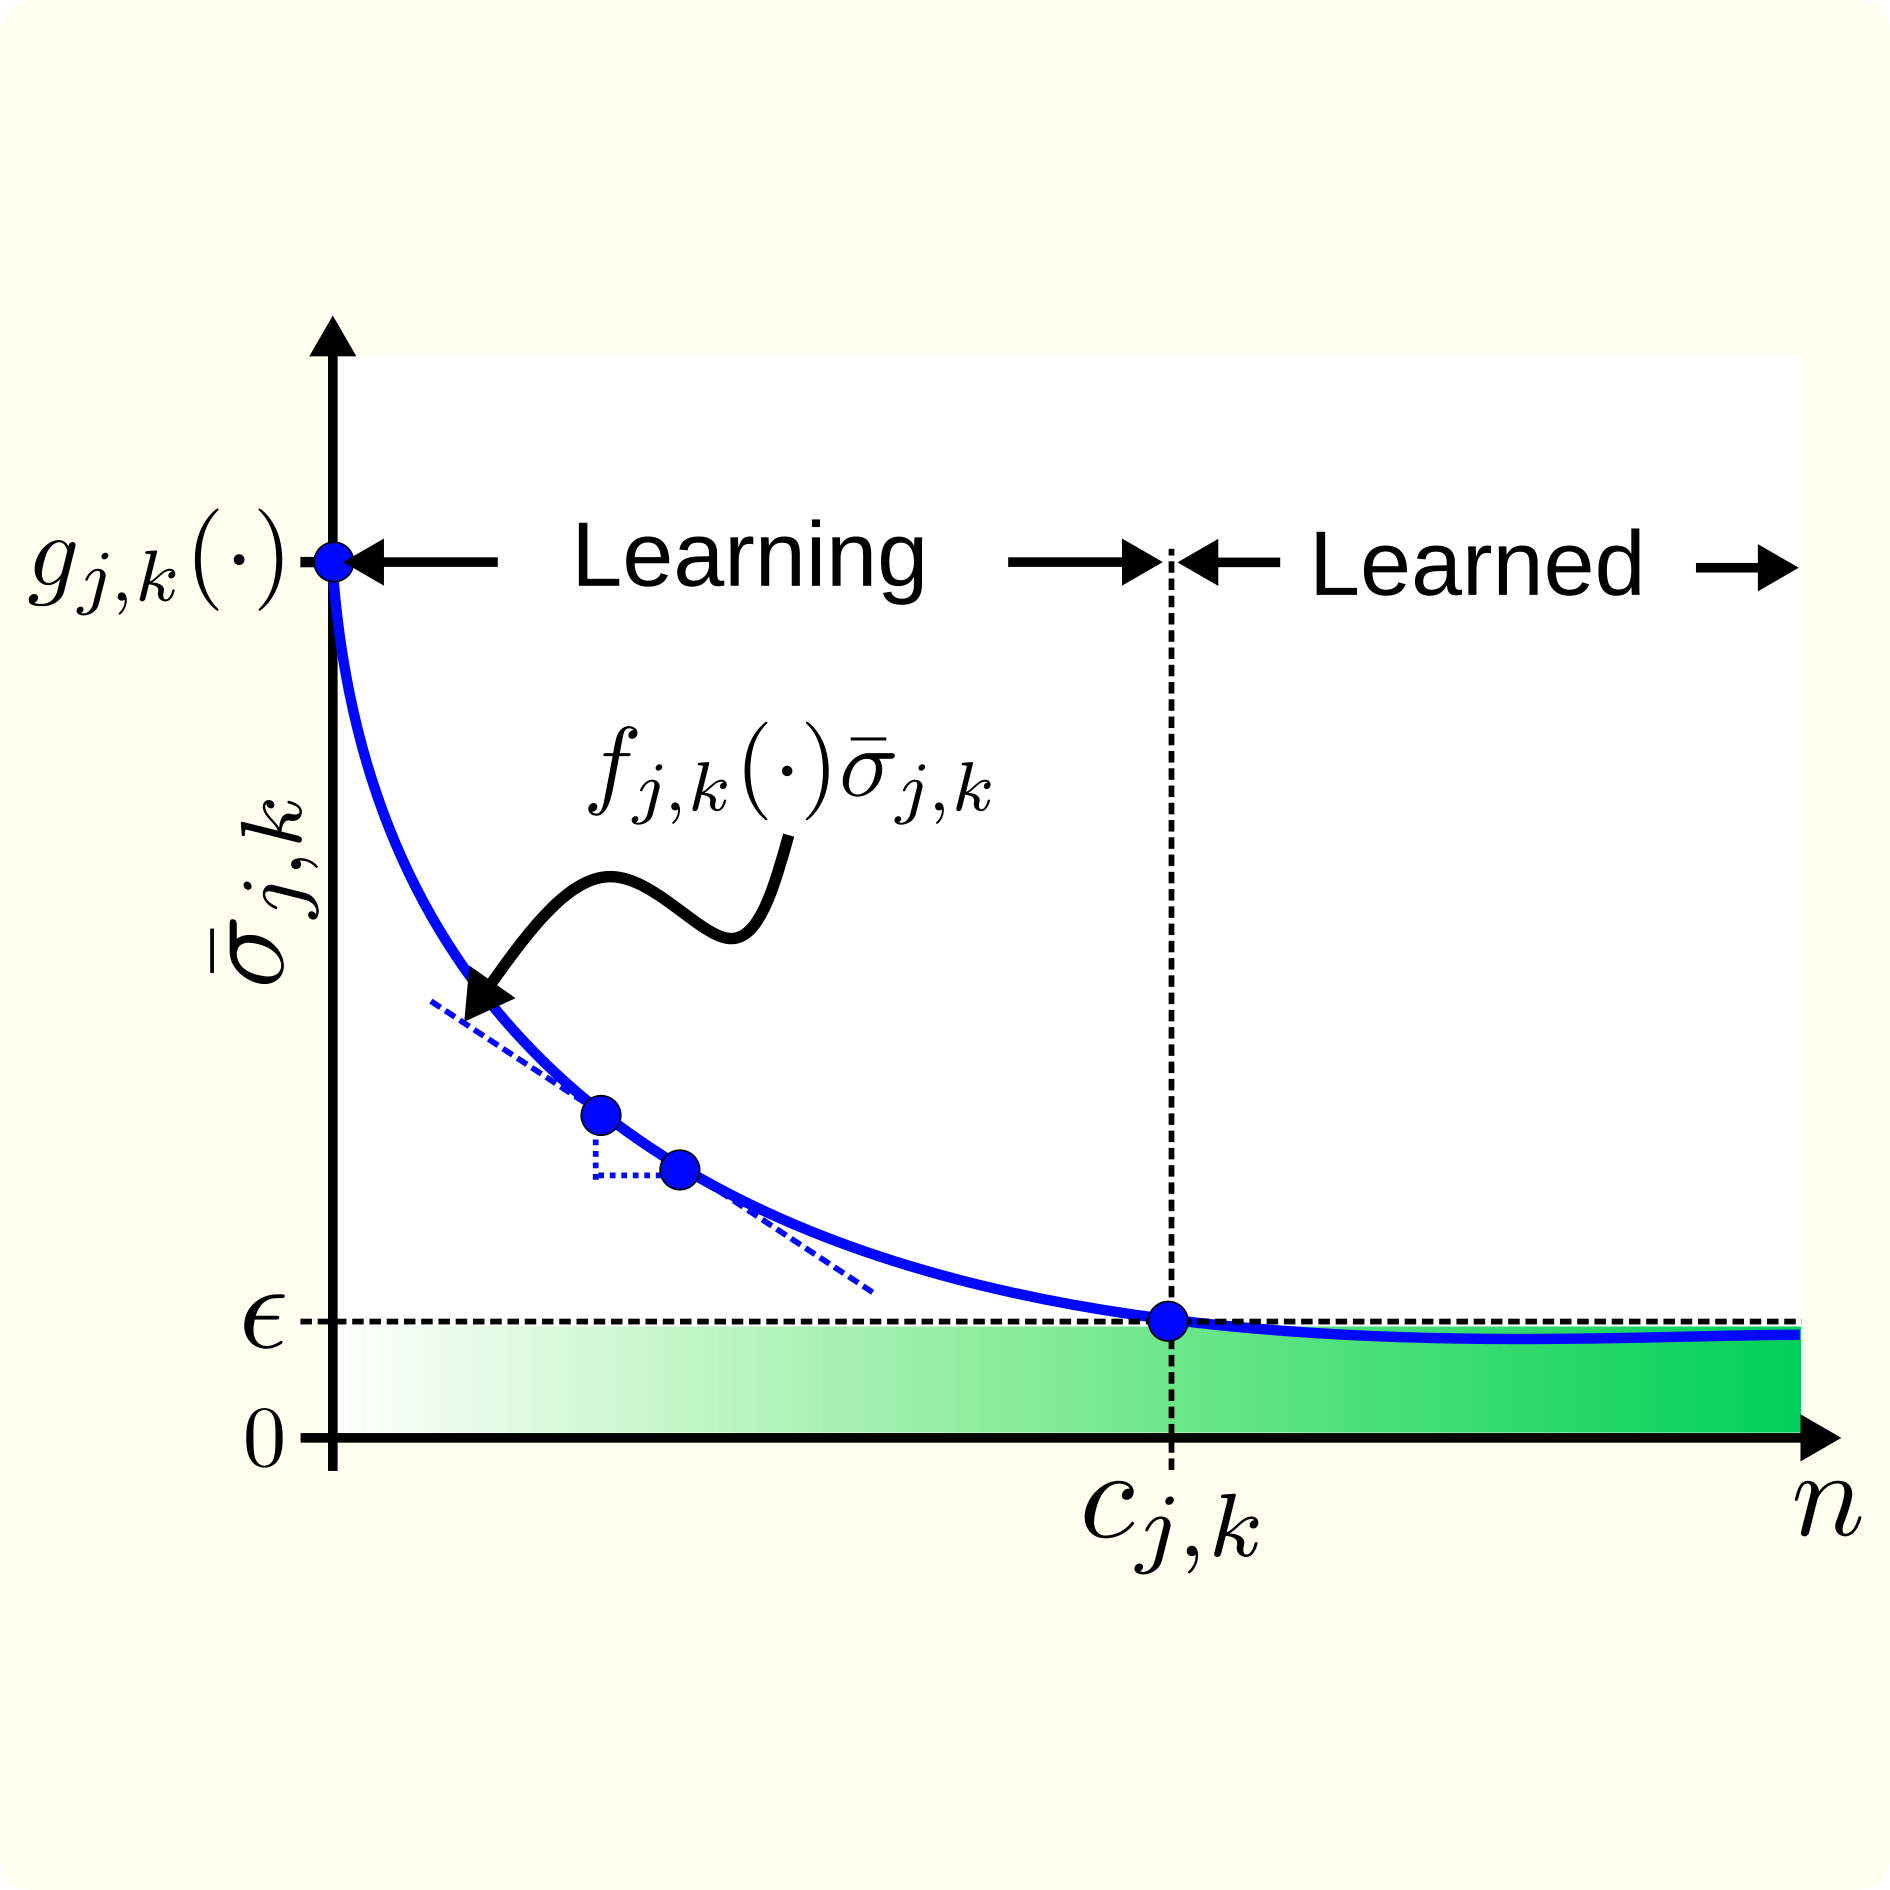
\includegraphics[width=\textwidth]{remaining_knowledge_dynamics_idealization.png} \label{fig:knowledge_idealization}
%	\end{subfigure}
%	\hspace*{\fill}
%	\caption[] {\label{fig:experimental_results} \textbf{Skill similarity and knowledge.} (\subref{fig:skill_similarity}) Skills in $\mathcal{S}$ inherently group into clusters $\mathcal{Z}_k$ based on their similarity, (\subref{fig:knowledge_idealization}) the remaining knowledge $\bar{\sigma}_{i,j}$ to learn a new skill $s_{j}$ has strictly monotonically decreasing behavior.}	
%\end{figure*}
%% ---


% ---
\begin{figure}[!t]
	\centering
	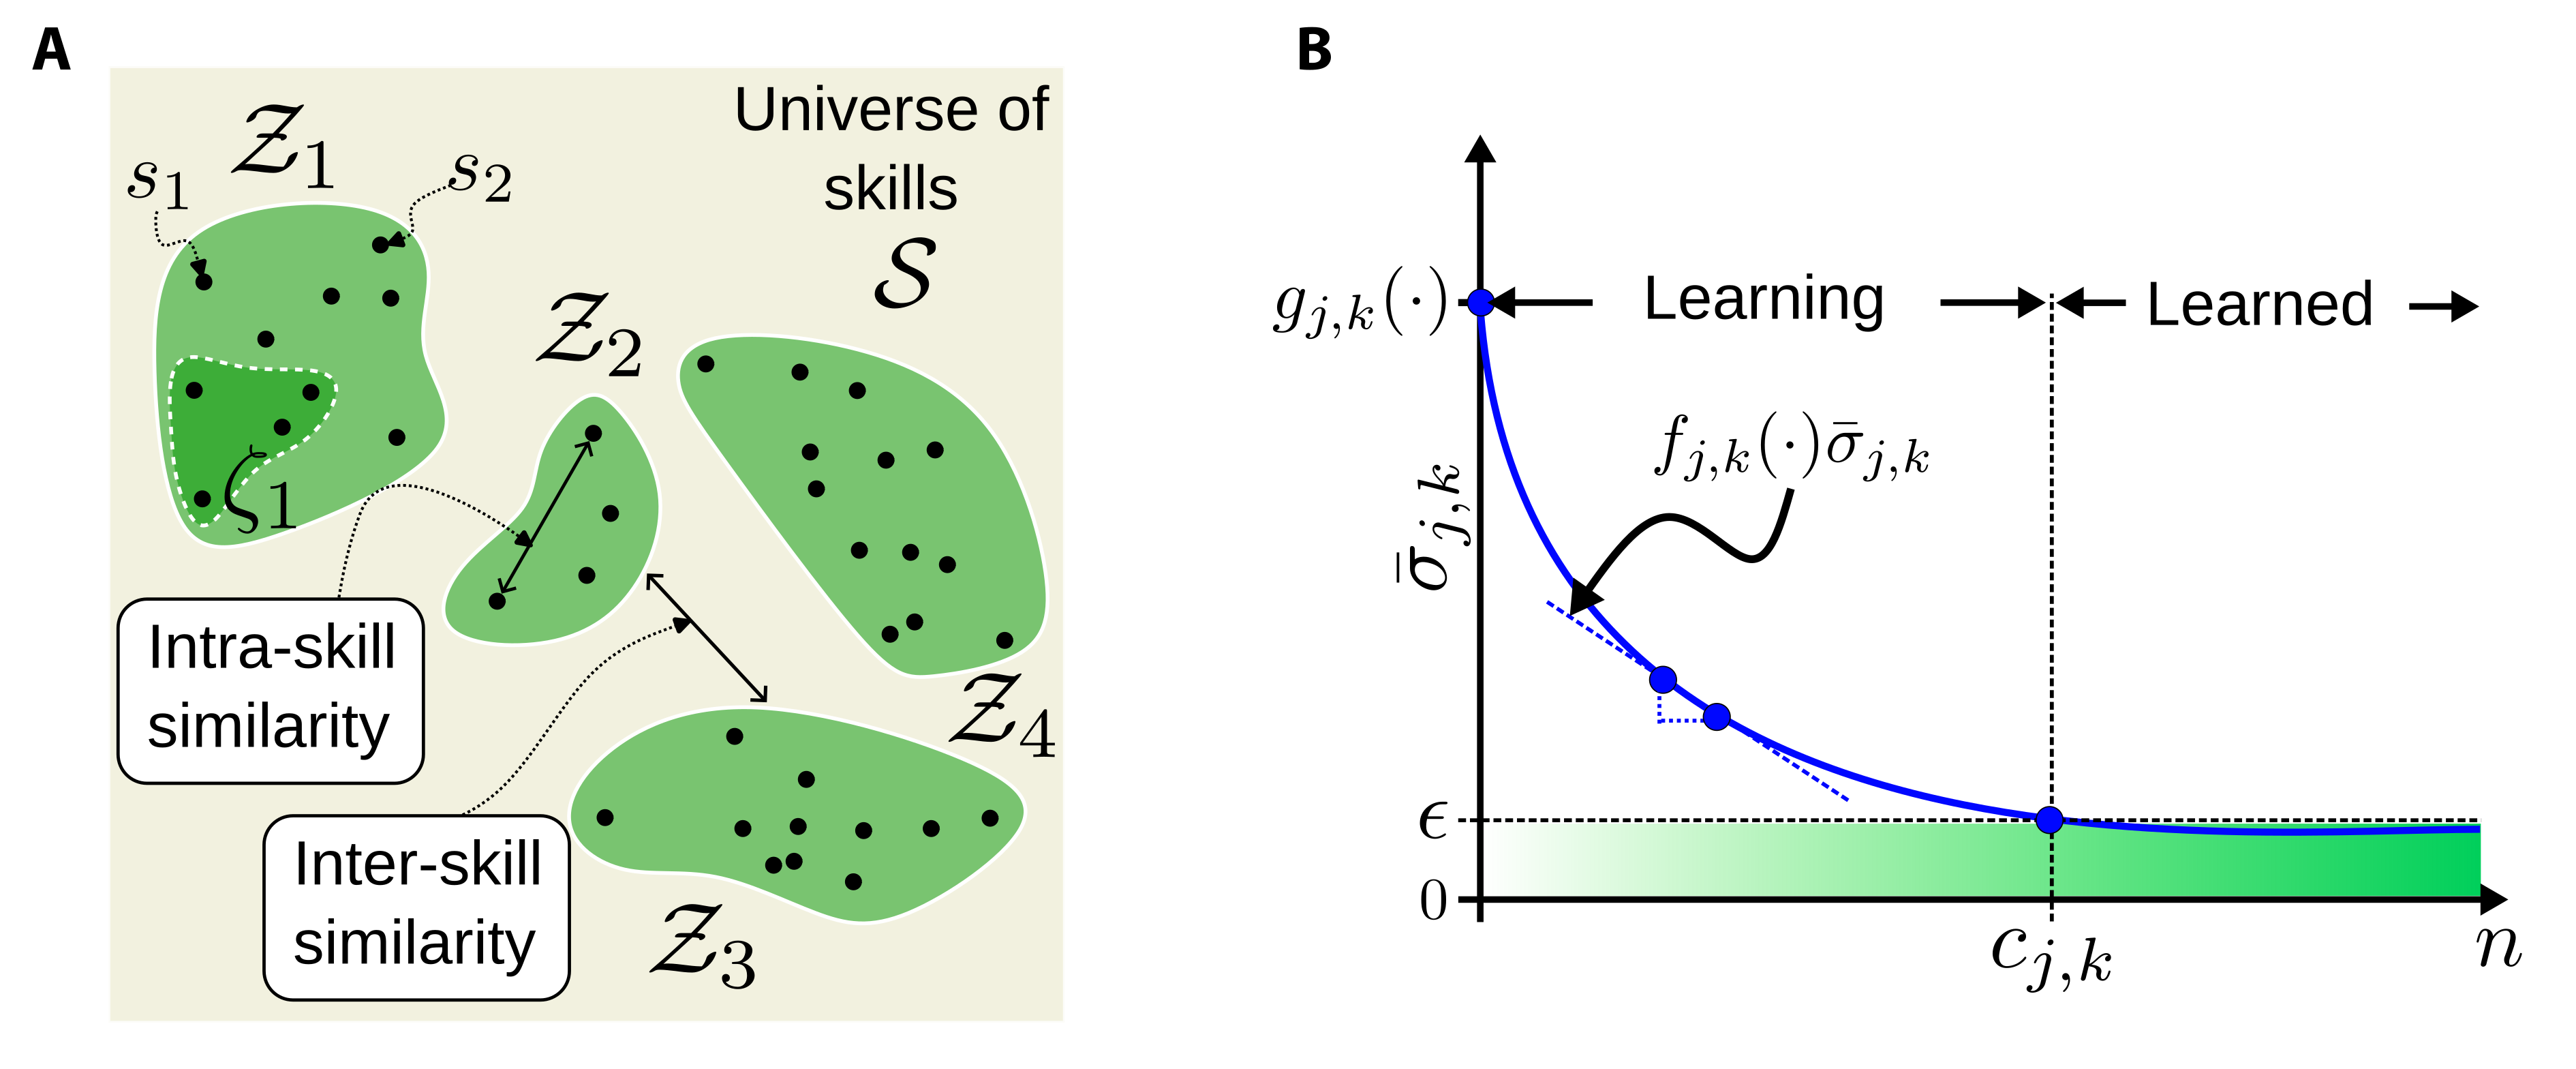
\includegraphics[width=0.95\textwidth]{fig/skill_similarity_and_knowledge.png}
	\caption{\textbf{Skill similarity and knowledge.} (\textbf{A}) Skills in $\mathcal{S}$ inherently group into clusters $\mathcal{Z}_k$ based on their similarity, (\textbf{B}) the remaining knowledge $\bar{\sigma}_{i,j}$ to learn a new skill $s_{j}$ has strictly monotonically decreasing behavior.}
    \label{fig:skill_similarity_and_knowledge} 
\end{figure}
% ---

To evaluate the effect of knowledge exchange during learning on the complexity of mastering a skill, we introduce a hypothetical upper bound called the skill \textit{fundamental complexity} $c_0$, which describes the maximum number of trial episodes required to learn \emph{any} skill. If, in learning a skill $ s_{j} $, the $i$-th \ac{eai} agent accesses and uses its knowledge contained in $\mathcal{\zeta}_k$, then two effects occur:
% ---
\begin{enumerate}
	\item There is less remaining knowledge, reflected in the initial value; i.e., $\bar{\sigma}_{i,j}(0) < 1$
	\item The knowledge acquisition rate increases. Equivalently, this may also be interpreted as an increase in the depletion rate of the remaining knowledge.
\end{enumerate}
% ---
These effects signify that the remaining knowledge scales down as a function of the number $N_{\zeta_k}=|\mathcal{\zeta}_k|$ of skills an agent has already learned. Consequently, the complexity $c_{j}$ of said skill is smaller than the fundamental complexity $c_0$. Additionally, without loss of generality, under knowledge exchange, we can consider that
% ---
\begin{tcolorbox}
	\begin{assumption}\label{assumption:exponential_decrease} the remaining knowledge function $\bar{\sigma}_{i,j}(\cdot)$ has stritctly monotonically decreasing behavior.
	\end{assumption}
\end{tcolorbox} 
% ---
\noindent An idealization of the behavior satisfying Asm.~\ref{assumption:exponential_decrease} and Eq.~\eqref{eq:sigma_bar_conditions} can be modeled by a dynamical system depending on the trial episodes $n$ and parameterized by the number of already learned skills $N_{\zeta_k}$. As such,
% ---
\begin{definition}\label{assumption:ode_model} the remaining knowledge function $\bar{\sigma}_{i,j}$ is modeled as the first order dynamical system
%	\begin{subequations}\label{eq:simple_knowledge_dynamics}
%		\begin{empheq}[left=\empheqlbrace]{align}
%			\dot{\bar{\sigma}}_{j,k}\left(n\right) &  = -f_{j,k} \left(N_{\zeta_k} \right) \bar{\sigma}_{j,k}\left(n\right),\\
%			\bar{\sigma}_{j,k}(0) &  =  g_{j,k} \left(N_{\zeta_k}\right).
%		\end{empheq}
%	\end{subequations}
	\begin{equation}\label{eq:simple_knowledge_dynamics}
		\dot{\bar{\sigma}}_{i,j}\left(n\right)=\begin{cases}
			-f_{i,j} \left(N_{\zeta_k} \right) \bar{\sigma}_{i,j}\left(n\right), & \epsilon < \bar{\sigma}_{i,j}\left(n\right) < 1, \\
			0, & \text{otherwise}.
		\end{cases}
	\end{equation}	
\end{definition}
% * NOTE: the subindex j,k means skill j in cluster k
% ---
\noindent Considering its initial condition as $\bar{\sigma}_{i,j}(0) =  g_{i,j} \left(N_{\zeta_k}\right)$, the corresponding solution
% ---
\begin{equation}\label{eq:knowledge_exponential_form}
	\bar{\sigma}_{i,j}(n) = g_{i,j}(N_{\zeta_k}) e ^{-f_{i,j}\left(N_{\zeta_k}\right) n} \in (0,1],
\end{equation}
% ---
exhibits the desired behavior, shown in Fig.~\ref{fig:skill_similarity_and_knowledge}~\textbf{B}. The function $f_{i,j}\left(N_{\zeta_k}\right)$ models one of the effects resulting from the exploitation of the knowledge available in $\zeta_k$, namely, the increase of the learning rate. The second effect, namely, the reduction in the initial remaining knowledge $\bar{\sigma}_{i,j}(0)$ is controlled by the term $g_{i,j}\left(N_{\zeta_k}\right)$, which is also dependent on the number of learned skills. The learning threshold $\epsilon$---depicted as the green-shaded area---indicates when the remaining knowledge is negligible and $s_{j}$ is considered to have been learned.

% % ===================================================================================================
% \paragraph*{Knowledge sharing under different learning paradigms}
In the remainder of our discussion, we consider an idealized reference system in which many robots coexist, learning numerous skills. Such system exhibits
% ---
\begin{tcolorbox}
	\begin{assumption}\label{assumption:average_behavior}
		an average behavior that results from comparable \ac{eai} agents learning and executing the skills in $\mathcal{S}$ ordered and segregated according to their similarity.
	\end{assumption}
\end{tcolorbox}
%---
\noindent Each of the \ac{eai} agents in the system
\begin{tcolorbox}
	\begin{assumption}\label{assumption:agent_similarity}
		has the same capabilities, with highly similar \ac{bee} and \ac{mie} expenditures.
	\end{assumption}
\end{tcolorbox}
%---
\noindent The large number of skills in $\mathcal{S}$ implies that
% ---
\begin{tcolorbox}
	\begin{assumption}\label{assumption:cluster_size}
		every cluster $\mathcal{Z}_{k}$ contains the same number $N_{\mathcal{Z}} $ of skills.
	\end{assumption}
\end{tcolorbox}
% ---
\noindent By virtue of the optimal ordering of the skills and the balanced size of the clusters,
% ---
\begin{tcolorbox}
	\begin{assumption}\label{assumption:cluster_transferability}
		the knowledge transferability between in-cluster skills---modeled by Eq.~\eqref{eq:f_function_incremental} and Eq.~\eqref{eq:g_function_incremental}---is assumed to be equal; as is transferability between clusters, see Eq.~\eqref{eq:f_function_transfer} and Eq.~\eqref{eq:g_function_transfer}.
	\end{assumption}
\end{tcolorbox}
% ---
\noindent Finally, the different learning paradigms that exploit the collected knowledge by the \ac{eai} agents rely on the assumption that
% ---
\begin{tcolorbox}
	\begin{assumption}\label{assumption:enabling_agorithms}
		there are advanced control and machine learning algorithms readily available to inherently use this knowledge.
	\end{assumption}
\end{tcolorbox}
% ---

% ---
%\begin{figure*}[!t]
%	\centering
%	\hspace*{\fill}
%	\begin{subfigure}[t]{0.32\textwidth}
%		\subcaption{}
%		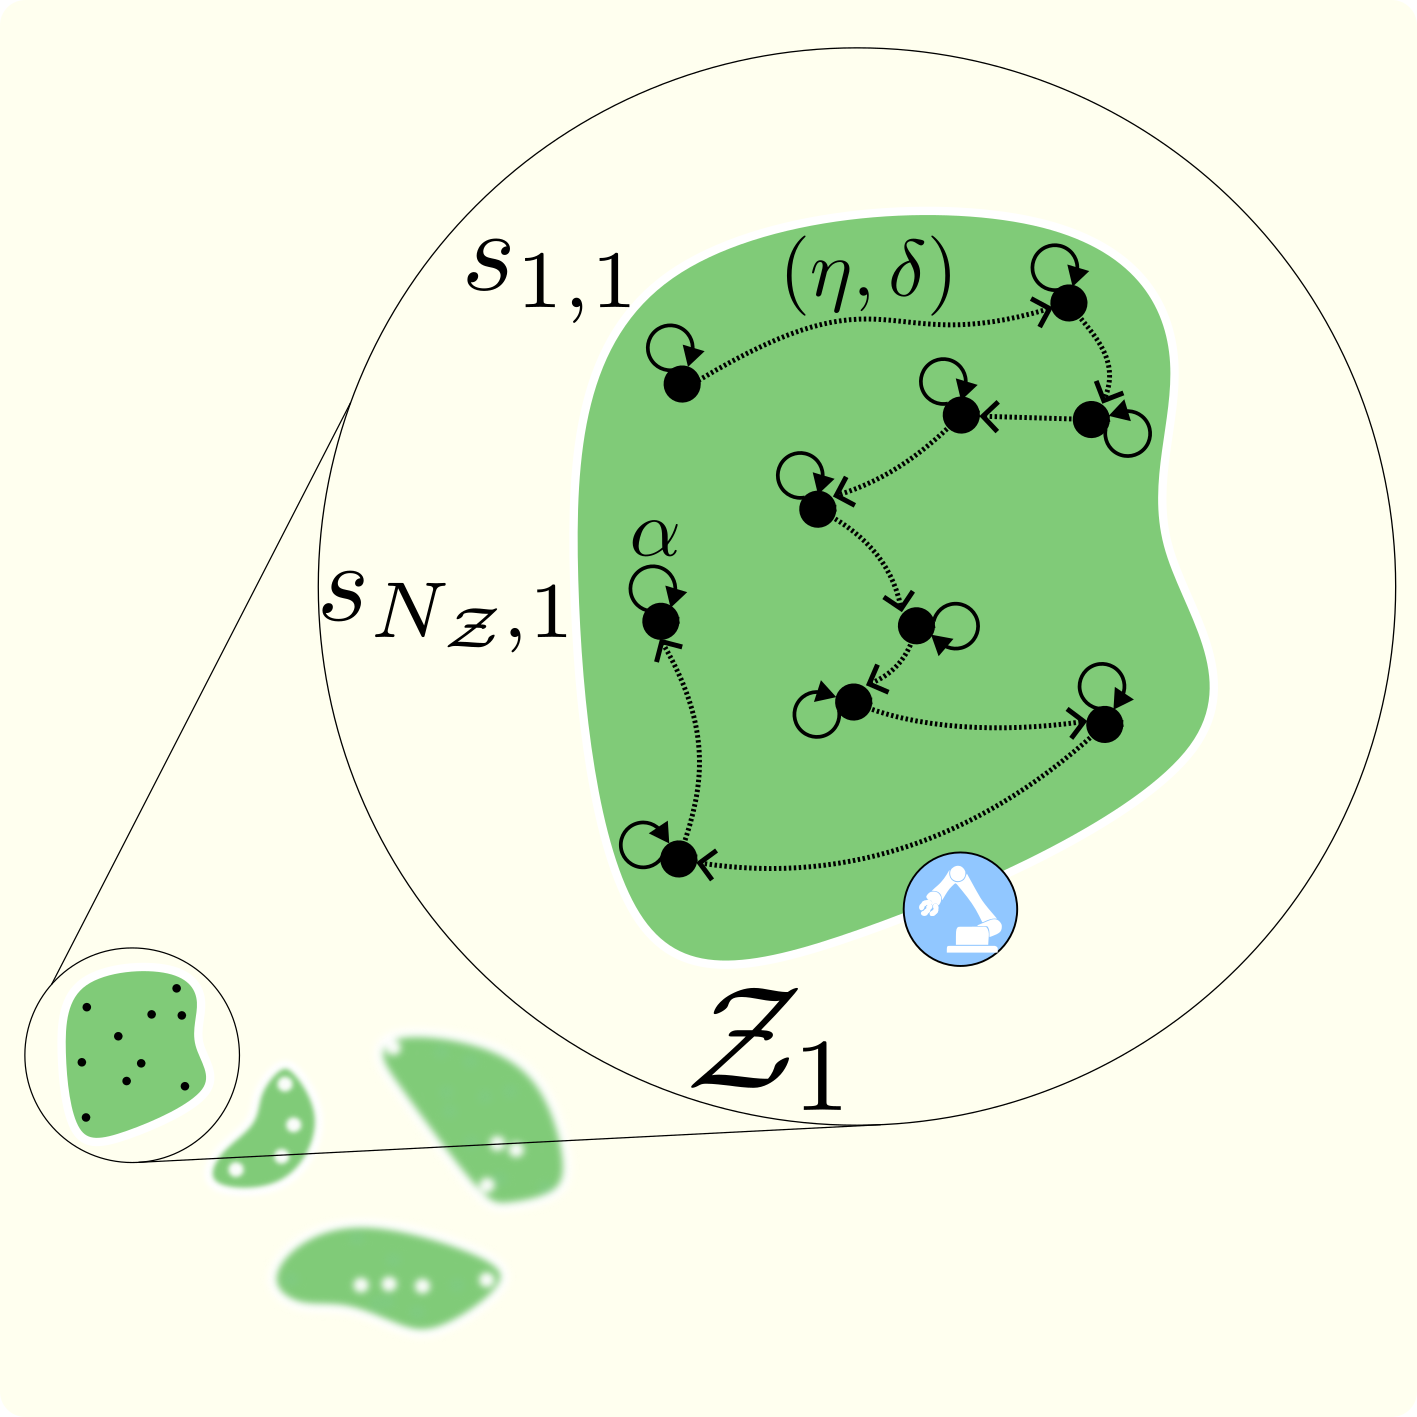
\includegraphics[width= \textwidth]{intra_skill_learning.png} \label{fig:intra_skill_learning}
%	\end{subfigure}
%	\hfill
%	\begin{subfigure}[t]{0.32\textwidth}
%		\subcaption{}
%		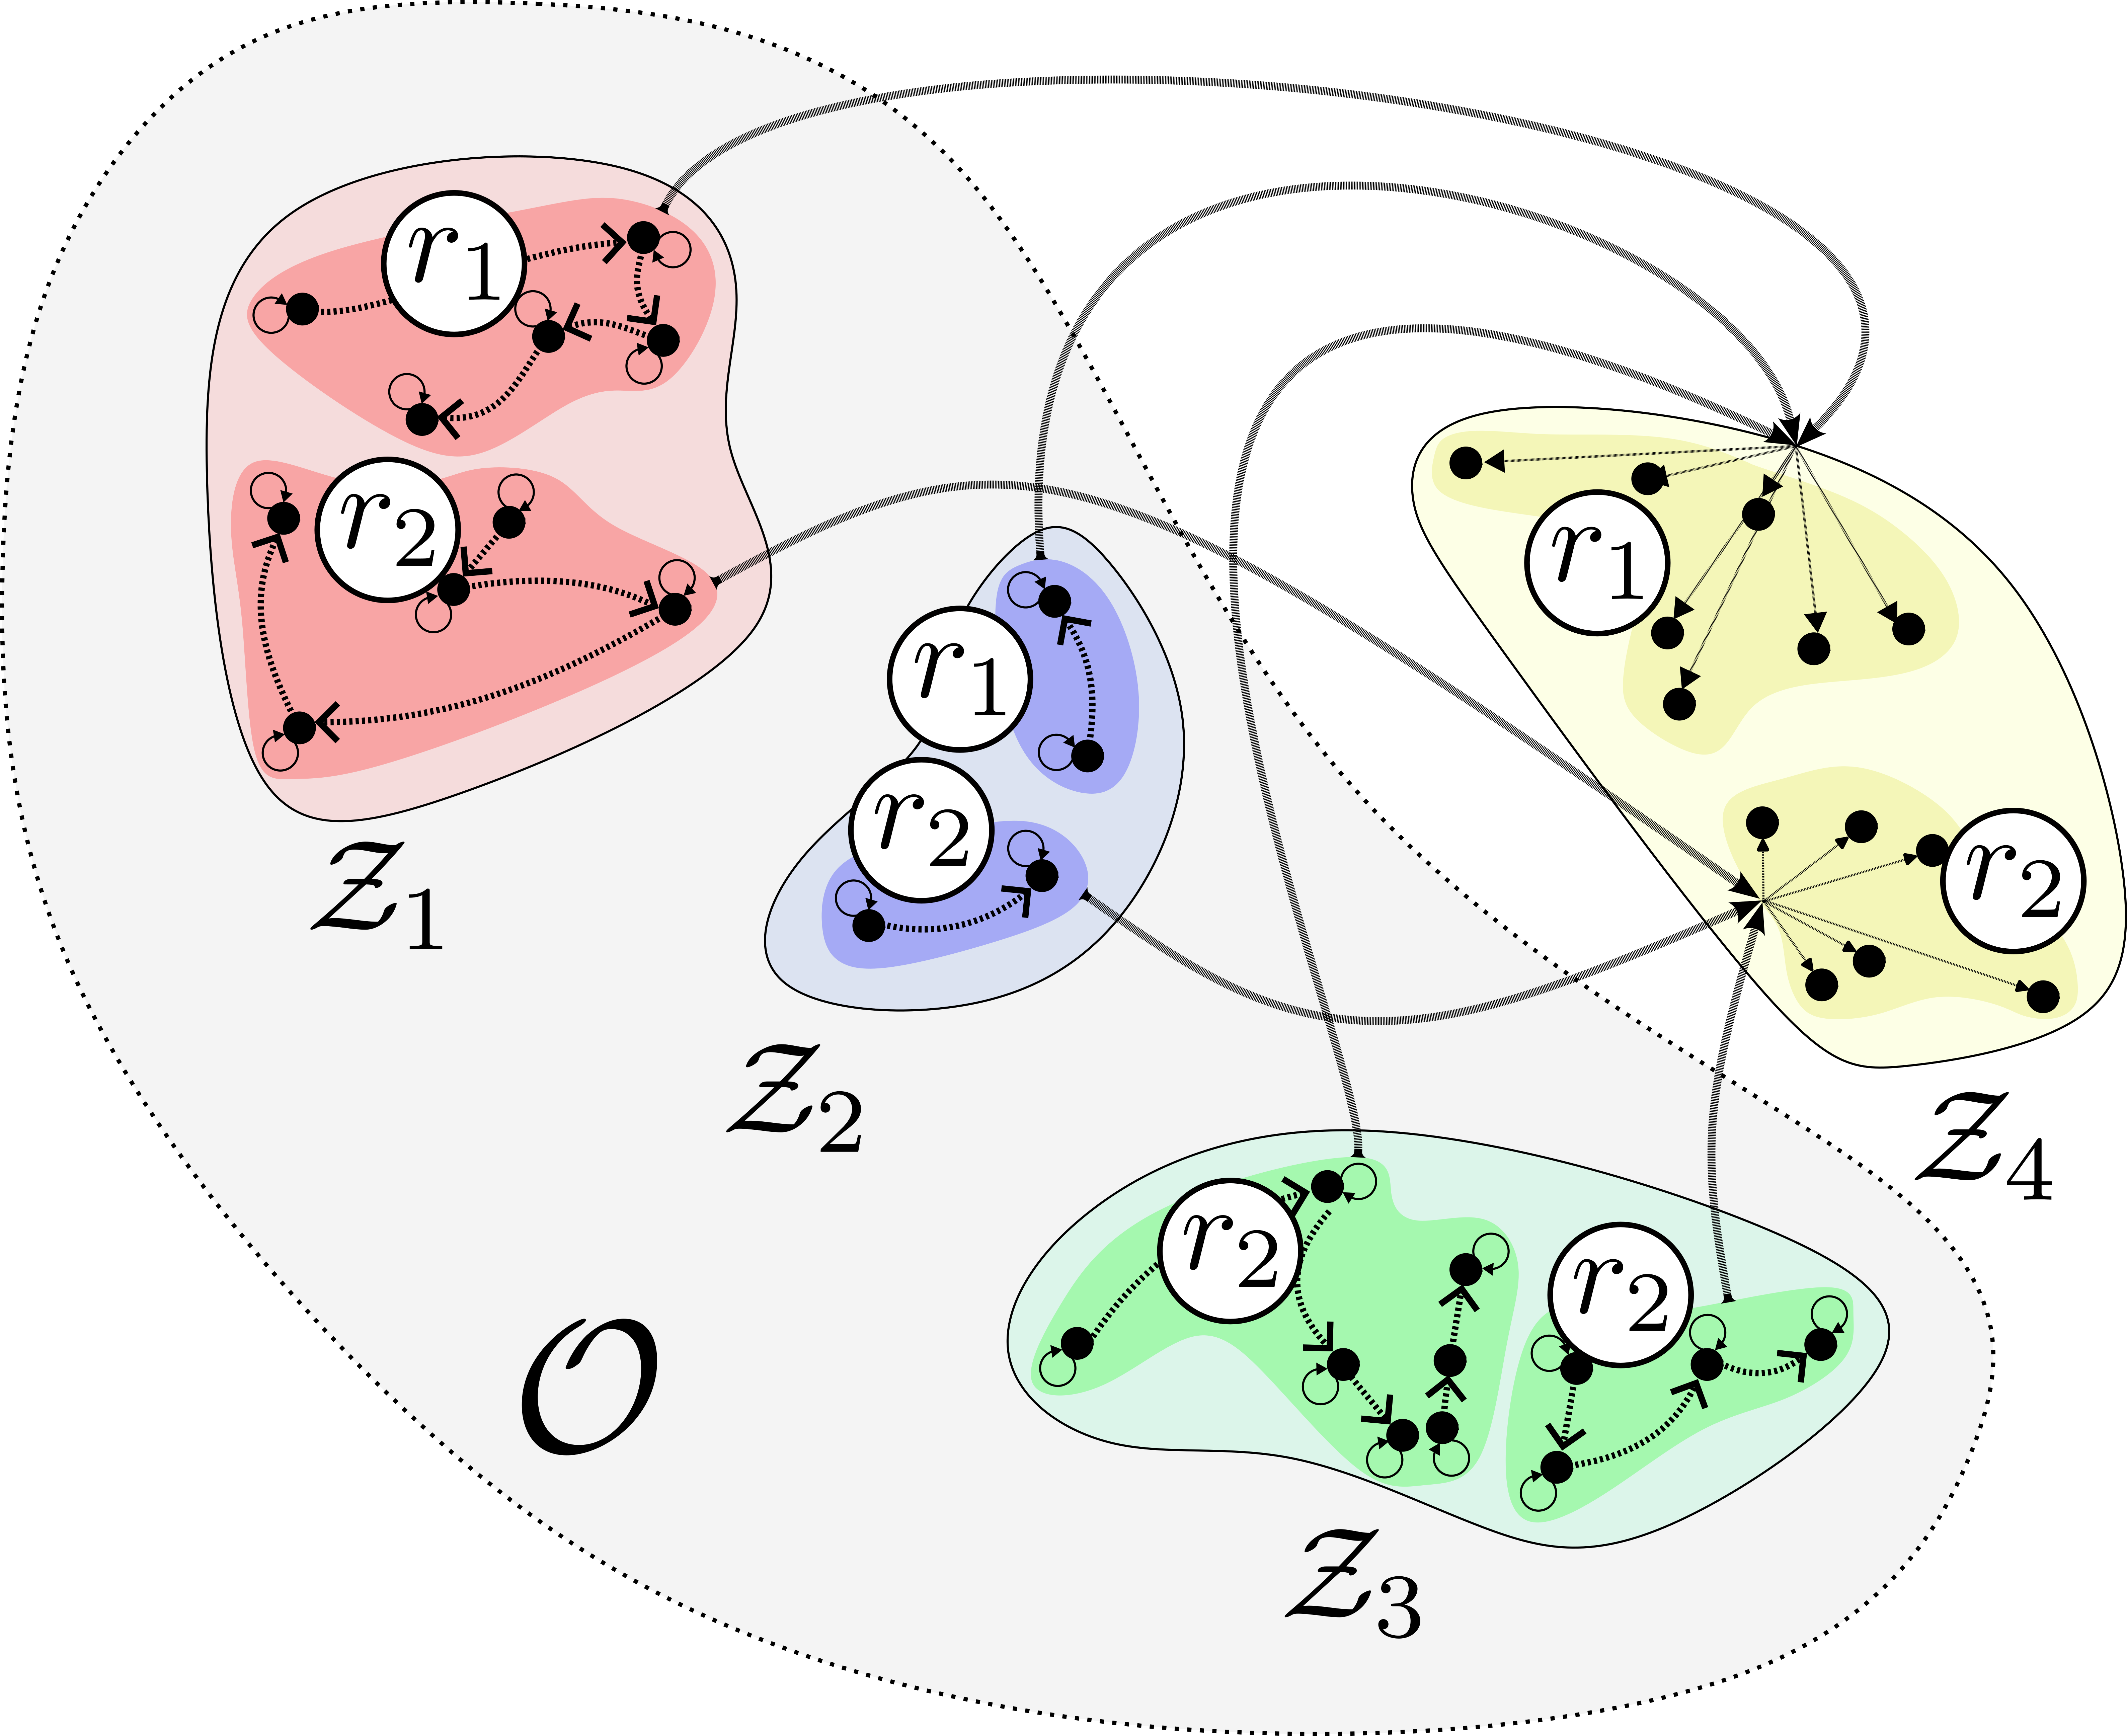
\includegraphics[width=\textwidth]{cluster_to_cluster_knowledge_transfer_parallel.png} \label{fig:cluster_to_cluster_knowledge_transfer_parallel}
%	\end{subfigure}
%	\hfill
%	\begin{subfigure}[t]{0.32\textwidth}
%		\subcaption{}
%		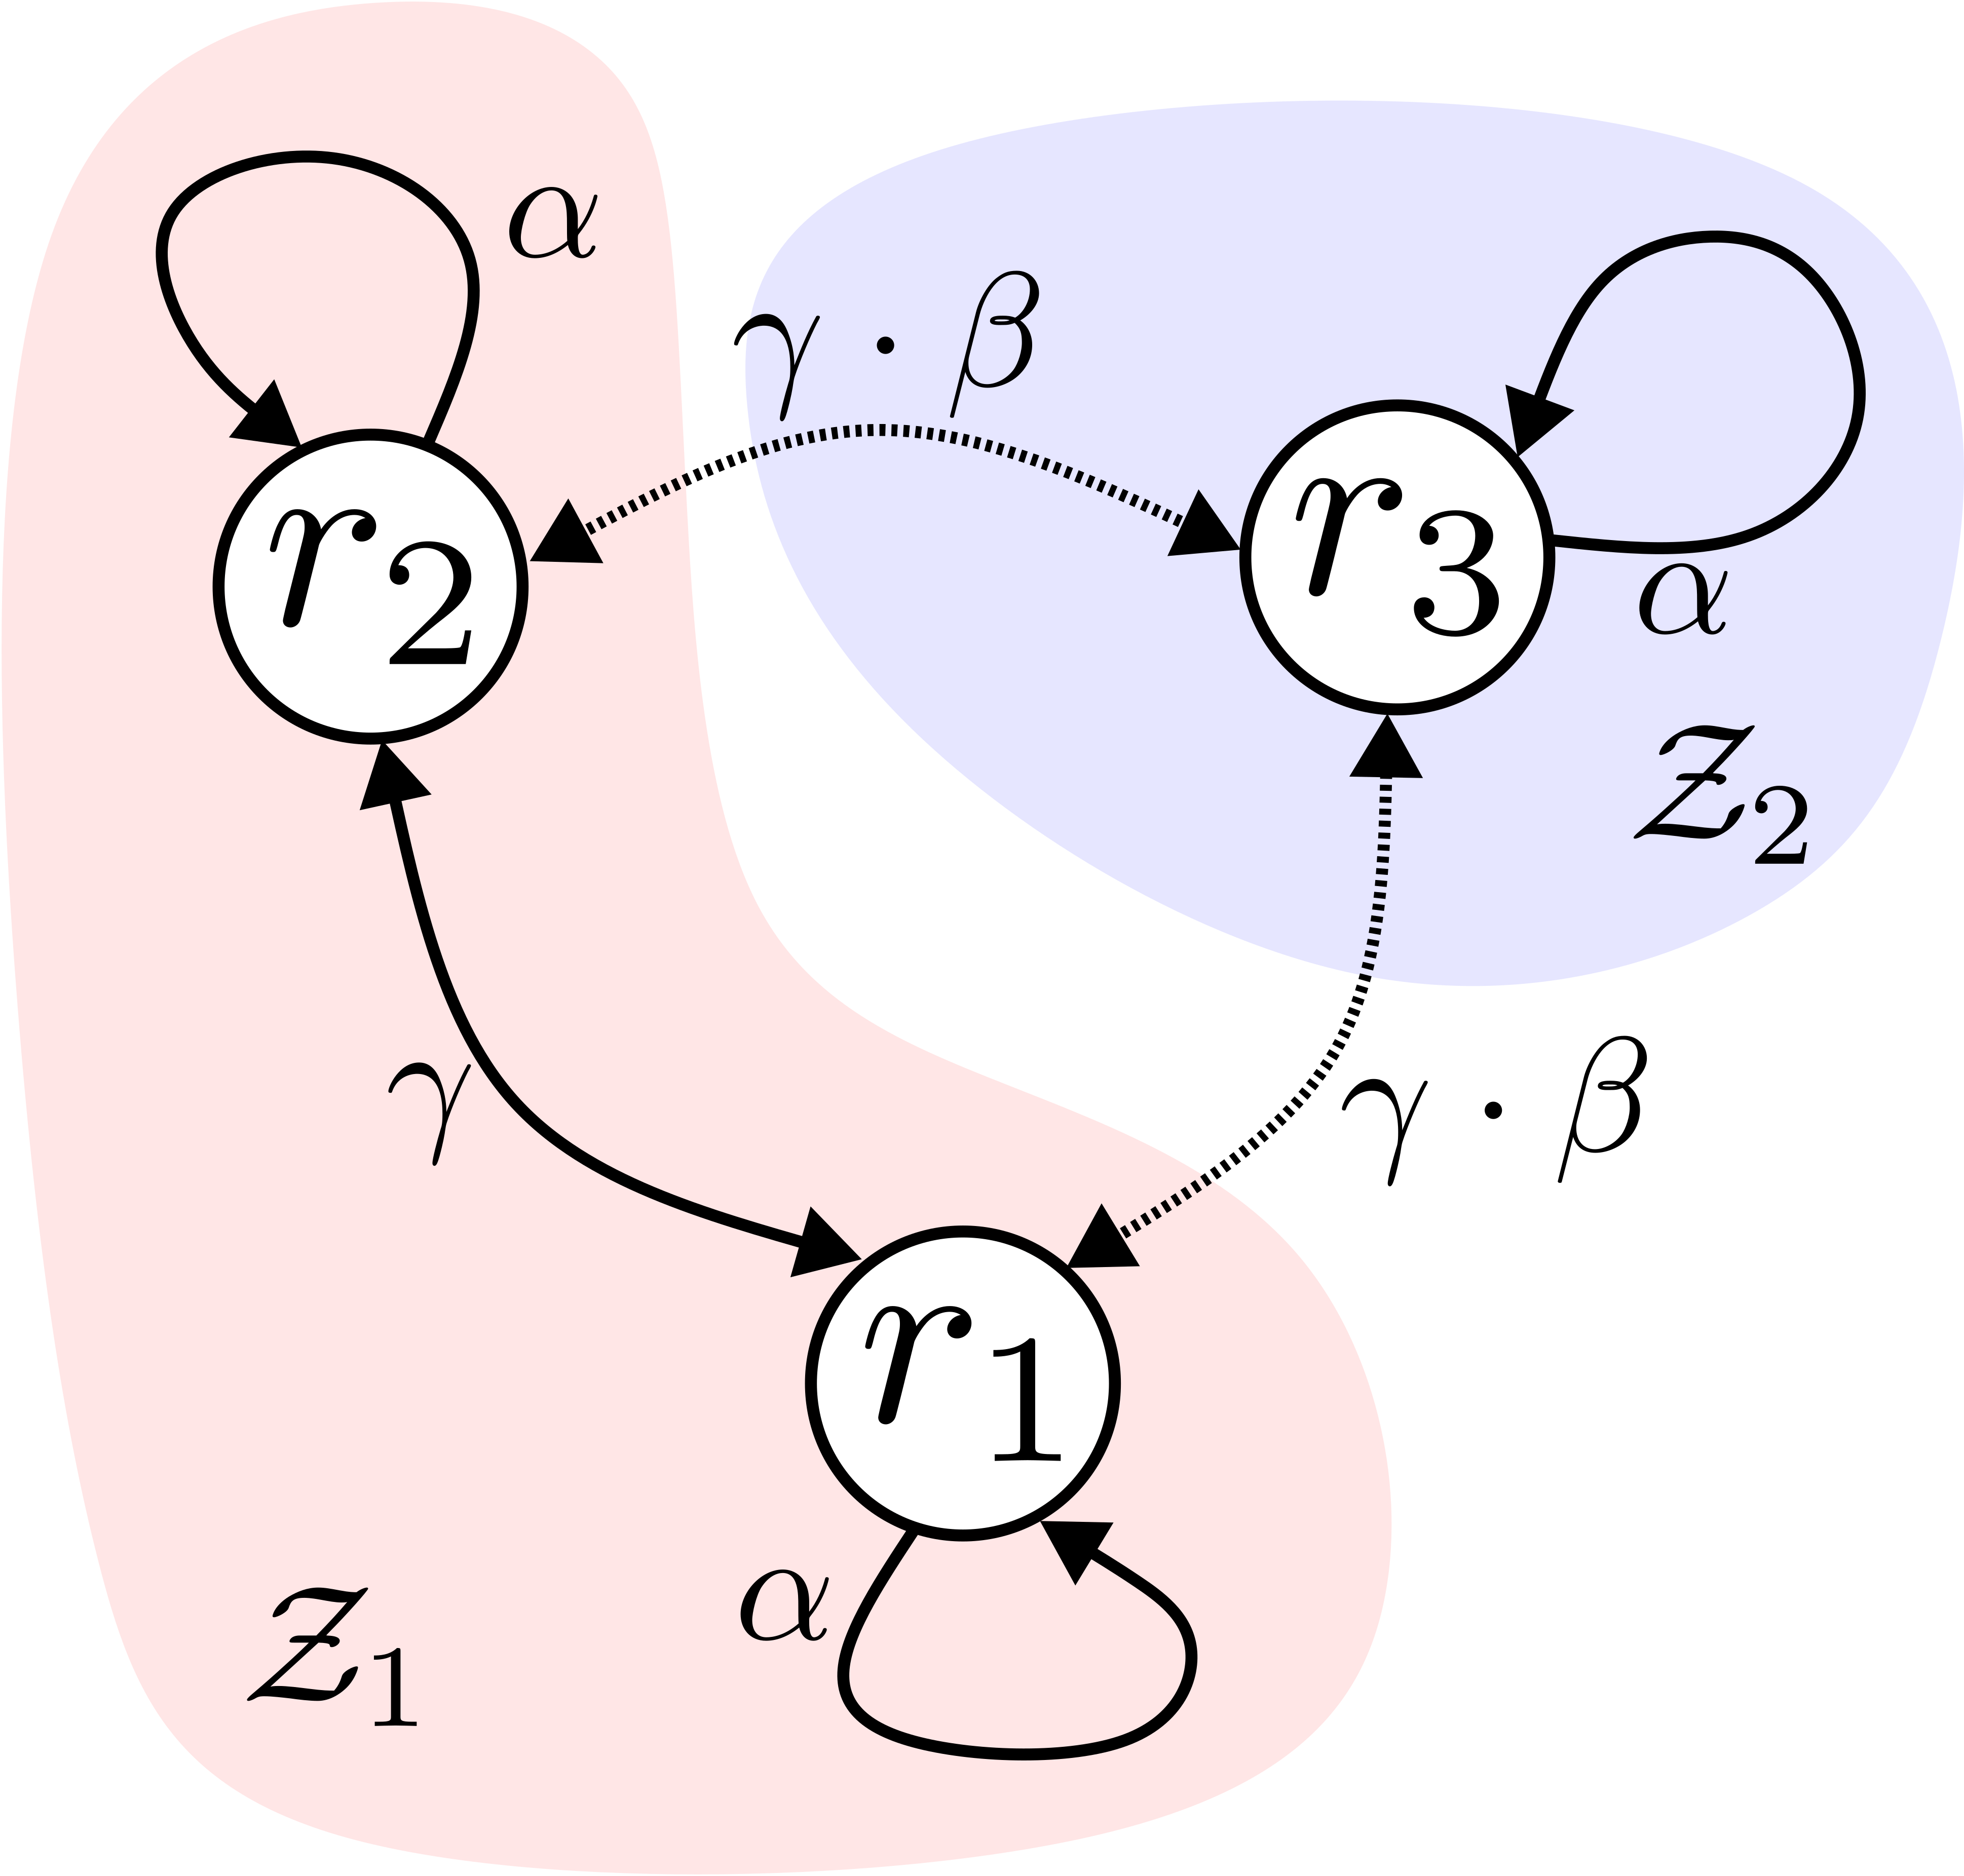
\includegraphics[width=\textwidth]{cl_example_figure.png} \label{fig:cl_example_figure}
%	\end{subfigure}	
%	\hspace*{\fill}
%	\caption[] {\label{fig:learning_paradigms_conceptual_figure} \textbf{The different learning paradigms.} (\subref{fig:intra_skill_learning}) \Acl{il} benefits from the significant similarity of skills belonging to the same cluster. (\subref{fig:cluster_to_cluster_knowledge_transfer_parallel}) In \acl{tl}, knowledge is shared from various source clusters to a target cluster. Notice that using many robots (e.g., two robots $r_1$ and $r_2$) without inter-agent knowledge exchange among them only subdivides the problem. (\subref{fig:cl_example_figure}) Exchange of knowledge between \ac{eai} agents enables \acl{cl}.}
%\end{figure*}
% ---

% ---
\begin{figure}[!t]
	\centering
	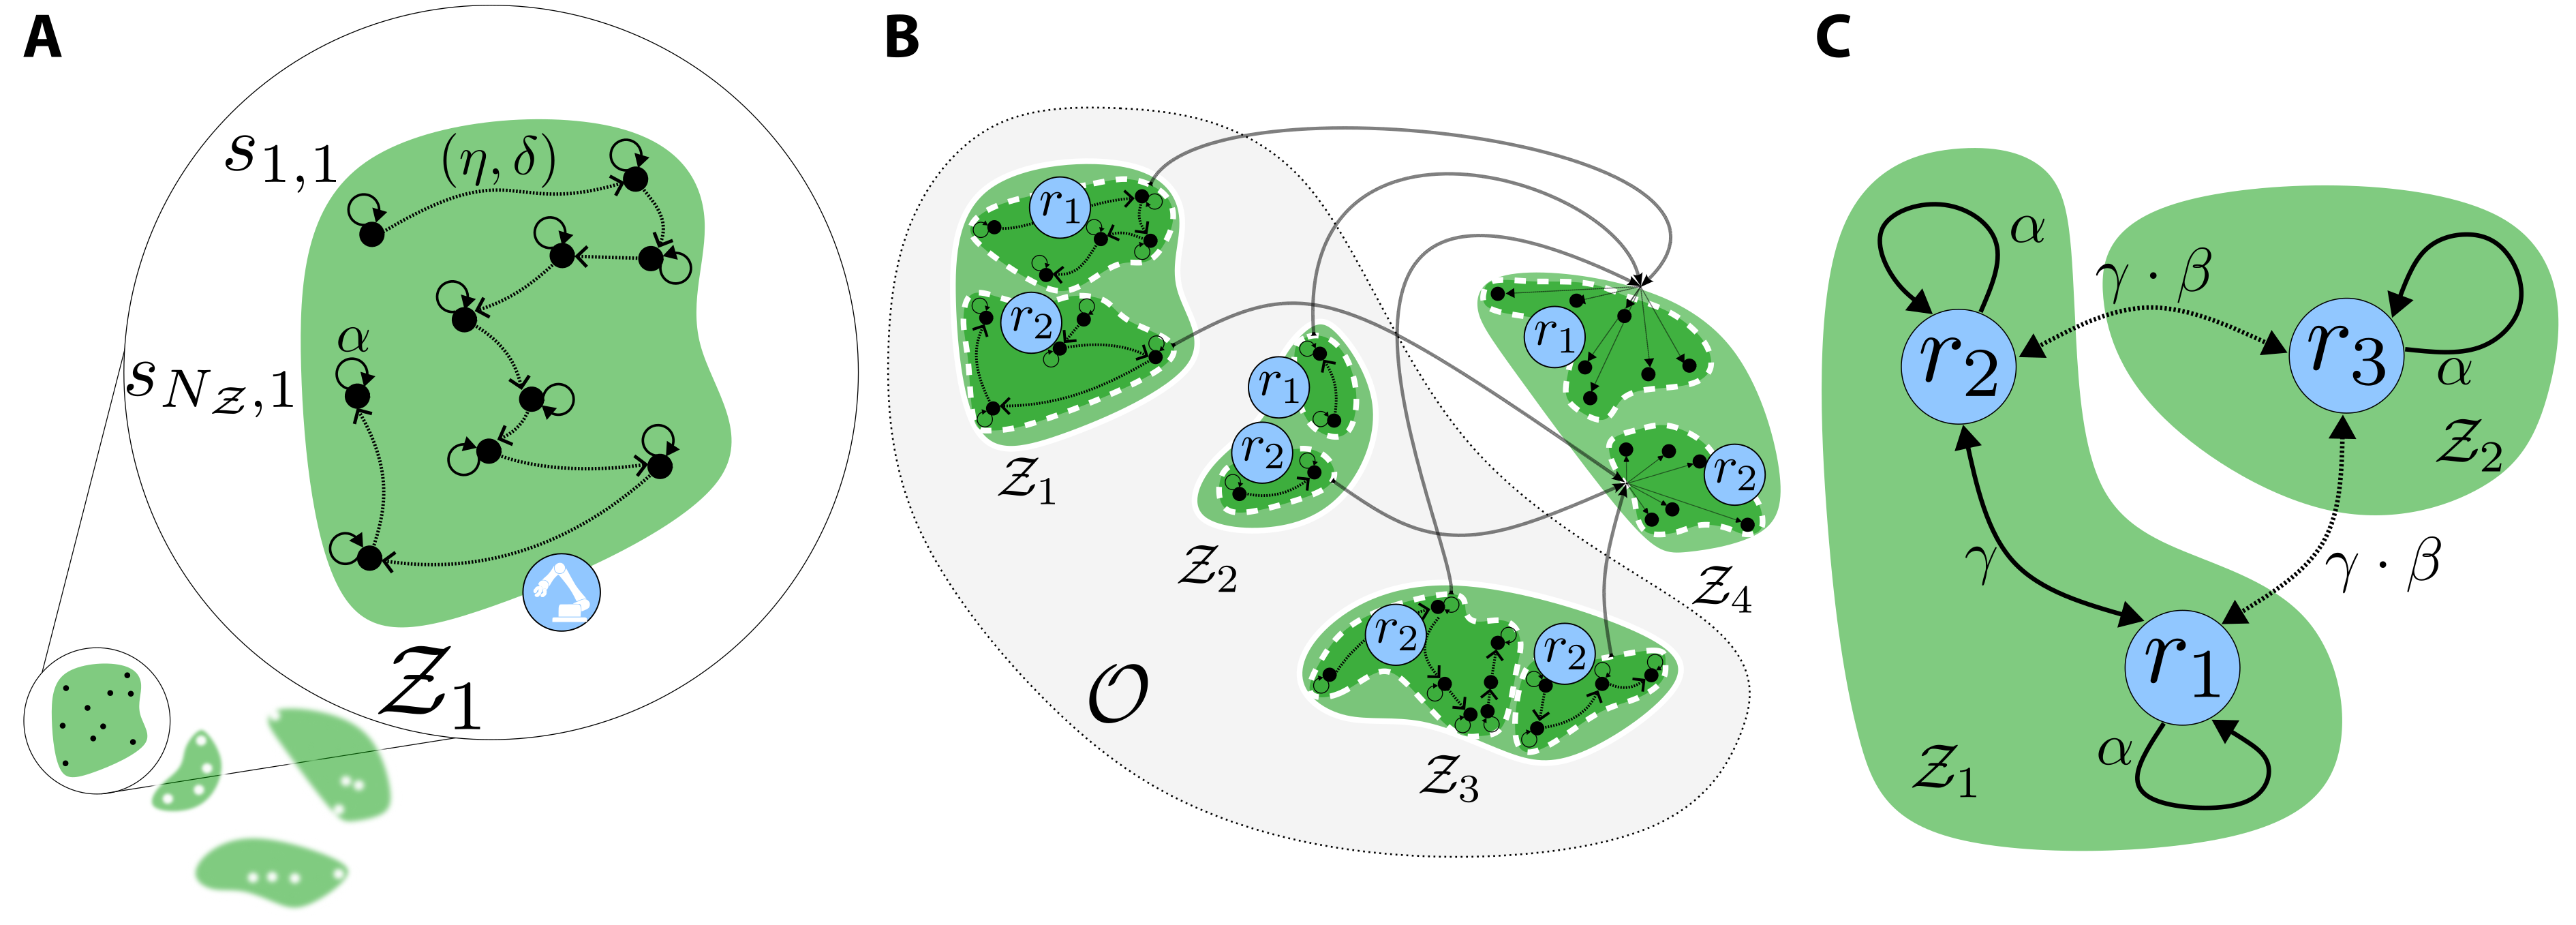
\includegraphics[width=0.95\textwidth]{fig/learning_paradigms_conceptual_figure.png}
	\caption{\label{fig:learning_paradigms_conceptual_figure} \textbf{The different learning paradigms.} (\textbf{A}) \Acl{il} benefits from the significant similarity of skills belonging to the same cluster. (\textbf{B}) In \acl{tl}, knowledge is shared from various source clusters to a target cluster. Notice that using many robots (e.g., two robots $r_1$ and $r_2$) without inter-agent knowledge exchange among them only subdivides the problem. (\textbf{C}) Exchange of knowledge between \ac{eai} agents enables \acl{cl}.}
\end{figure}
% ---

% ===================================================================================================
\paragraph*{Knowledge sharing under different learning paradigms}
When an \ac{eai} agent learns in isolation---that is, performs \ac{isl}---it learns every skill from the ground up, disregarding knowledge from already learned skills. In contrast, during \ac{il}---also known as continual learning \cite{Lesort2020Continuallearningrobotics}---an agent benefits from the continuous aggregation and exchange of knowledge from \emph{intra-cluster} skills in virtue of their significant similarity. As depicted in Fig.~\ref{fig:learning_paradigms_conceptual_figure}~\textbf{A}, a robot ($r_1$ in this case) learns every skill in $\mathcal{Z}_1$ with a rate $\alpha$---the self-learning loops---but also retains the acquired knowledge in its local memory and uses it to learn subsequent skills. \Ac{tl} alone refers to the use of acquired knowledge about a distant set of skills on a new skill \cite{Hosna2022Transferlearningfriendly,Jaquier2023TransferLearningRobotics}. In particular, it implies the one-time \emph{inter-cluster} exchange of knowledge. \Ac{tl} represents the exchange of knowledge from the skills learned in different \emph{origin} clusters $\mathcal{O} = \{ \mathcal{Z}_1,\mathcal{Z}_2,\ldots,\mathcal{Z}_{k-1} \}$ to the skills that will be learned in a \emph{destination} cluster $\mathcal{Z}_k$ (see Fig.~\ref{fig:learning_paradigms_conceptual_figure}~\textbf{B}). Concretely, the effect that \ac{tl} has on the skills of the destination cluster is the reduction of the initial remaining knowledge and the increase of the initial learning rate for all the skills in the target cluster through \emph{transferable knowledge fraction factor} $\xi_k \in [0,1)$. The latter results from aggregating the available knowledge $\varsigma^{(k)}$ that an agent has in memory about each of the $N_\mathcal{K}$ clusters weighted by the \emph{cluster similarity matrix}
% ---
\begin{equation}\label{eq:cluster_similarity_matrix}
	\bm{B}\in \mathbb{R}^{N_\mathcal{K} \times N_\mathcal{K}}=\begin{cases}
		1, & i=j, \\
		\beta_{i,j} = \beta_{j,i}, & i \neq j.
	\end{cases}
\end{equation}
% ---
Here, $\beta_{i,j} \in [0,1)$ defines the closeness between the skills in the different clusters (recall the dashed lines in  Fig.~\ref{fig:collective_learning_and_skill_manifold_conceptualization}~\textbf{A}). In general, \ac{il} and \ac{tl} are ideally combined; as such, we consider \ac{til} as the third learning paradigm. A complementary discussion about the effects of these paradigms on the skill complexity is provided in the \nameref{sec:supplementary_materials}.

% In general, \ac{il} and \ac{tl} can always be combined; as such, we consider \ac{til} as the third learning paradigm. A complementary discussion on the effects that these paradigms have on the skill complexity is provided in Sec.~\ref{sec:materials_and_methods} of the \nameref{sec:supplementary_materials}.

% ===================================================================================================
\paragraph*{\textbf{\Acl{cl}}}
This paradigm goes far beyond simple parallelization, understood as learning different skills with different robots at the same time. In \ac{cl} $N_\mathrm{r}$ robotic agents $ \left\lbrace r_i \right\rbrace_{i=1}^{N_\mathrm{r}} $ develop and accumulate an emerging common mind (body of knowledge) dynamically via networked interactions where individual experience, knowledge, and skills are disseminated to all the other elements in the collective \cite{Garavan2012CollectiveLearning}. Information flows vertically as previous knowledge is passed on, automatically improving knowledge gaps in the skill tree, and horizontally by sharing concurrent experience between agents, to accelerate skill acquisition ``in action''. Knowledge can be replicated, complemented, and further developed via these mechanisms. Moreover, to enable \ac{cl} from a technical standpoint, it is assumed that an inter-agent communication protocol and the appropriate infrastructure are in place that allow agents to concurrently exchange and integrate the self-acquired and incoming knowledge to incrementally speed up the learning of all the agents as a whole. As a result, concurrent intra- and inter-cluster knowledge sharing is possible. Naturally, a complex scheduling problem to determine the optimal skill distribution and inter-agent knowledge-sharing strategy is part of the \ac{cl} paradigm. 

Rather than focusing on specific learning, communication, and scheduling algorithms to make \ac{cl} possible, our primary objective is to illustrate the overarching ideal systemic behavior of a \acl{cl}.~% system (see Fig.~\ref{fig:collective_learning_system}).
Grounded on Assumptions~\ref{assumption:average_behavior}, \ref{assumption:agent_similarity},~\ref{assumption:cluster_size}, and~\ref{assumption:cluster_transferability}, in the remainder of this work, we concentrate the discussion on the target knowledge-sharing dynamics of a \ac{cl} system. Figure~\ref{fig:learning_paradigms_conceptual_figure}~\textbf{C} illustrates the \ac{cl} concept, where the self-loop represents the knowledge dynamics of a single robot learning at a rate $\alpha$. The exchange of knowledge across agents is represented via the cross-couplings, weighted by a parameter $\gamma$ that models how efficient the bidirectional pairwise knowledge exchange is between any two agents. Similar to \ac{tl}, if two robots exchange knowledge about skills in different clusters $j$ and $l$, then $\gamma_{j,l}$ is scaled down by the cluster similarity $\beta_{j,l}$. 

In \ac{cl}, the dynamics of the remaining knowledge  about a skill acquired by an agent exchanging knowledge with a set $\mathcal{N}$ of other agents is described by
% ---
%\begin{equation}\label{eq:collective_knowledge_dynamics}
%	\dot{\bar{\sigma}}^{(\text{CL})}_{j,k} =
%	\begin{cases}
%		\overbrace{\left[-\alpha \left( \frac{\eta \kappa + 1}{1 - \xi_k} \right)  - \sum\limits_{l \in \mathcal{N}(j)} \beta_{j,l} \gamma_{j,l} d(\bar{\sigma}_j,\bar{\sigma}_l)\right]}^{f(\cdot)} \bar{\sigma}^{(\text{CL})}_{j,k}, & \epsilon < \bar{\sigma}_{j,k} < 1, \\
%		0, & \text{otherwise};
%	\end{cases}
%\end{equation}

% ---
\begin{equation}\label{eq:collective_knowledge_dynamics}
	\dot{\bar{\sigma}}^{(\text{CL})}_{i,j} =
		\overbrace{\left[-\alpha_i\:\left( \frac{\eta_i \kappa + 1}{1 - \xi_{i,j}(\bm{B},\bm{\varsigma}_i)} \right)  - \sum\limits_{l \in \mathcal{N}(j)} \bar{\xi}_{i,l}(\bm{B},\bm{v}) \gamma_{i,l} d(\bar{\sigma}_{i,j},\bar{\sigma}_{l,\cdot})\right]}^{\textbf{learning rate}} \bar{\sigma}^{(\text{CL})}_{i,j},
\end{equation}
% ---
\noindent for $\epsilon < \bar{\sigma}_{i,j} < 1$ and with \textbf{initial condition} $\bar{\sigma}^{(\text{CL})}_{i,j}(0) = g_{i,j}\left(\kappa\right)$. Note that $\kappa$ represents the total number of successfully learned skills. Without knowledge sharing, $\kappa= N_{\zeta_k}$, with $N_{\zeta_k}$ being the number of skills already learned in the cluster of skill $s_j$. In \ac{cl}, ideally $\kappa$ is equal to all the skills learned by the robots in the collective up to the current learning cycle. However, it is possible that some agents may fail to successfully learn a given skill.

Each gain $\gamma_{i,l} \in \mathbb{R} $ weighs the knowledge exchange strength among robots. Since robots may have in-memory skills from different clusters, the transferable knowledge fraction factor is given by
% ---
\begin{equation}\label{eq:scaled_transferable_knowledge_fraction}
	{\xi}_{i,j} = \mathbb{1}^\intercal_j\:(\bm{B} - \bm{I})\:\bm{\varsigma}_i ,
\end{equation}
% ---
\noindent~where $\mathbb{1}_j \in \mathbb{R}^{N_\mathcal{K}}$ is a one-hot vector representing the cluster to which skill $s_j$ belongs. In the absence of knowledge sharing, the entries of vector $\bm{\varsigma}_i \in \mathbb{R}^{N_\mathcal{K}}$ are the knowledge fraction from each skill cluster that agent $i$ holds in memory. In contrast, when operating as a collective, $\bm{\varsigma}_i$ contains the aggregated cluster knowledge fraction gathered by all the agents. The expression in Eq.~\eqref{eq:scaled_transferable_knowledge_fraction} accounts for the one-time transfer of knowledge based upon the cluster similarity at the beginning of a learning cycle. Similarly, the term $ \bar{\xi}_{i,l}(\bm{B},\bm{v}) $ downsizes the concurrent---that is, during learning---sharing of knowledge coming from the skills currently being learned in different clusters. The vector $\bm{v} \in \mathbb{R}^{N_\mathrm{r}}$ describes the cluster membership of each of the skills in the current skill batch learned by the $N_\mathrm{r}$ agents. 




% In \ac{cl}, after a learning cycle, ideally $\kappa= N_\mathrm{r} N_{\zeta_k}$. However, since some agents may fail to successfully learn a given skill, then $\kappa \leq N_\mathrm{r} N_{\zeta_k}$.

The \emph{knowledge integration function} 
% ---
\begin{equation}\label{eq:knowledge_integration_function}
	d(\bar{\sigma}_{i,j},\bar{\sigma}_{l,\cdot}) = e^{-a\:\left(\bar{\sigma}_{l,\cdot}-\bar{\sigma}_{i,j}\right)^2}\in [0,1],
\end{equation}
% --- 
\noindent in Eq.~\eqref{eq:collective_knowledge_dynamics} accounts for the contribution of knowledge from other agents, weighing it according to the relevance (similarity) of the shared knowledge. 

% The functions
% \begin{equation}\label{eq:f_function_collective}
% 	f(\cdot) = -\alpha \left( \frac{\eta \kappa + 1}{1 - \xi_k} \right)  - \sum_{l \in \mathcal{N}(j)} \bar{\xi}_{j,l} \gamma_{j,l}d(\bar{\sigma}_j,\bar{\sigma}_l)
% \end{equation}

% % --- 
% \noindent and 
% % ---
% \begin{equation}%\label{eq:f_function_collective}
% 	g(\cdot) = (1-\xi_k) e^{-\delta \kappa}
% \end{equation}
% % ---
% \noindent are dependent on the number of successfully learned skills $ \kappa $ and the $N_\mathrm{r}$ knowledge-exchanging robots. Note that, after a learning cycle, ideally $\kappa= N_\mathrm{r} N_{\zeta_k}$; however, since some agents may fail to successfully learn a given skill, then $\kappa \leq N_\mathrm{r} N_{\zeta_k}$.

% The \emph{knowledge integration function} 
% % ---
% \begin{equation}\label{eq:knowledge_integration_function}
% 	d(\bar{\sigma}_j,\bar{\sigma}_l) = e^{-a\left(\bar{\sigma}_l-\bar{\sigma}_j\right)^2}\in [0,1],
% \end{equation}
% % --- 
% \noindent in Eq.~\eqref{eq:collective_knowledge_dynamics} accounts for the contribution of knowledge from other agents, weighing it according to the relevance (similarity) of the shared knowledge. 
%% ---
%\begin{table}[!t]
%	\caption{The dynamics of the learning paradigms.\label{tab:learning_paradigms_expressions}}
%	\begin{center}
%		\begin{adjustbox}{width=\textwidth}
%			\begin{tabular}{|l||*{4}{c|}}\hline
%				Learning paradigm
%				&\makebox[3em]{\ac{isl}}&\makebox[3em]{\ac{il}}&\makebox[3em]{\ac{til}}
%				&\makebox[3em]{\ac{cl}}\\\hline\hline
%				Rate $f_{j,k}\left(\cdot \right)$  &$ \alpha$ & $ \alpha\left(\eta N_{\zeta_k} + 1 \right)$ & $\alpha \left( \frac{\eta N_{\zeta_k} + 1}{1 - \beta_k} \right)$ & $  h_{j,k}\left(N_{\zeta_k},\alpha,\eta,\beta_k,r\right)  - \beta_k \sum_{l \in \mathcal{N}(j)}\gamma_{j,l}d(\bar{\sigma}_j,\bar{\sigma}_l)$ \\\hline
%				Initial condition $g_{j,k}\left(\cdot \right)$ &$1$ & $e^{-\delta N_{\zeta_k}}$ & $(1-\beta_k) e^{-\delta N_{\zeta_k}}$ & $(1-\beta_k) e^{-\delta \kappa} $ \\\hline
%			\end{tabular}
%		\end{adjustbox}
%	\end{center}	
%\end{table}
%% ---
%% ---
%\begin{table}[!t]
%	\caption{The dynamics of the learning paradigms.\label{tab:learning_paradigms_expressions}}
%	\begin{center}
%		\begin{adjustbox}{width=\textwidth}
%			\begin{tabular}{|l||*{4}{c|}}\hline
%				Learning paradigm
%				&\makebox[3em]{\ac{isl}}&\makebox[3em]{\ac{il}}&\makebox[3em]{\ac{til}}
%				&\makebox[3em]{\ac{cl}}\\\hline\hline
%				Rate $f_{j,k}\left(\cdot \right)$  &$ \alpha$ & $ \alpha\left(\eta N_{\zeta_k} + 1 \right)$ & $\alpha \left( \frac{\eta N_{\zeta_k} + 1}{1 - \beta_k} \right)$ & $  \alpha \left( \frac{\eta r N_{\zeta_k} + 1}{1 - \beta_k} \right)  - \beta_k \sum_{l \in \mathcal{N}(j)}\gamma_{j,l}d(\bar{\sigma}_j,\bar{\sigma}_l)$ \\\hline
%				Initial condition $g_{j,k}\left(\cdot \right)$ &$1$ & $e^{-\delta N_{\zeta_k}}$ & $(1-\beta_k) e^{-\delta N_{\zeta_k}}$ & $(1-\beta_k) e^{-\delta \kappa} $ \\\hline
%			\end{tabular}
%		\end{adjustbox}
%	\end{center}	
%\end{table}
%% ---
% % ---
% \begin{table}[!t]
% 	\caption{The dynamics of the learning paradigms.\label{tab:learning_paradigms_expressions}}
% 	\begin{center}
% 		\begin{adjustbox}{width=\textwidth}
% 			\begin{tabular}{|l||*{4}{c|}}\hline
% 				\textbf{Learning paradigm}
% 				&\makebox[3em]{\textbf{\ac{isl}}}&\makebox[3em]{\textbf{\ac{il}}}&\makebox[3em]{\textbf{\ac{til}}}
% 				&\makebox[3em]{\textbf{\ac{cl}}}\\\hline\hline
% 				Rate $f_{j,k}\left(\cdot \right)$  &$ -\alpha$ & $ -\alpha\left(\eta \kappa + 1 \right)$ & -$\alpha \left( \frac{\eta \kappa + 1}{1 - \xi_k} \right)$ & $  -\alpha \left( \frac{\eta \kappa + 1}{1 - \xi_k} \right)  - \sum_{l \in \mathcal{N}(j)}\bar{\xi}_{j,l}\gamma_{j,l}d(\bar{\sigma}_j,\bar{\sigma}_l)$ \\\hline
% 				Initial condition $g_{j,k}\left(\cdot \right)$ &$1$ & $e^{-\delta \kappa}$ & $(1-\xi_k) e^{-\delta \kappa}$ & $(1-\xi_k) e^{-\delta \kappa} $ \\\hline
% 			\end{tabular}
% 		\end{adjustbox}
% 	\end{center}	
% \end{table}
% % ---

% More generally, the dynamics of the remaining knowledge for all the considered learning paradigms are captured in Eq.~\eqref{eq:collective_knowledge_dynamics} as described in Table~\ref{tab:learning_paradigms_expressions}. In summary, the model parameters have the following interpretations:
% % ---
% \begin{enumerate}
% 	\item The parameter $\alpha \sim \mathcal{U}(\alpha_{\text{min}},\alpha_{\text{max}}) \in \mathbb{R}_+$ accounts for different embodiments and models the \emph{base learning rate} at which a robot in isolation learns any given skill. According to Asm.~\ref{assumption:agent_similarity}, the range $[\alpha_{\text{min}},\alpha_{\text{max}}]$ is rather narrow.
% 	\item The parameter $\delta \in (0,\delta_{\text{max}}]$ reflects the intrinsic intelligence of the system and controls the \emph{exponential depletion rate}  of the initial remaining knowledge.
% 	\item The parameter $\eta \sim \mathcal{N}(\bar{\eta},\eta_{\Sigma})$ is the \emph{intra-cluster knowledge exchange factor}, it models the efficient use of experience (e.g. accessing memory) and represents the efficiency of knowledge exchange from $\zeta_k$ to $s_{j,k}$.
% 	\item The parameter $\gamma \sim \mathcal{N}(\bar{\gamma},\gamma_\Sigma)$ is the \emph{inter-agent knowledge exchange factor}, it weighs the knowledge exchange between agents and accounts for different embodiments, false communication, and dissimilar knowledge.
% %	\item $\beta_k$ is the head start granted by knowledge transfer from other clusters to the skills in $\mathcal{Z}_k$.
% \end{enumerate}
% % ---

% ===================================================================================================
%                                                 |                                                 |
%                                                 |                                                 |
% -------------------------------------------- SECTION ---------------------------------------------|
%                                                 |                                                 |
%                                                 |                                                 |
% ===================================================================================================
\section*{Supplementary Materials}
Sections \ref{sec:energy_time_and_power_per_episode} to \ref{sec:technical_data_and_references}\\
Fig.~\ref{fig:power_per_episode} to Fig.~\ref{fig:cobot_watt_per_kg}

% ===================================================================================================
%                                                 |                                                 |
%                                                 |                                                 |
% -------------------------------------------- SECTION ---------------------------------------------|
%                                                 |                                                 |
%                                                 |                                                 |
% ===================================================================================================
\renewcommand\refname{References and Notes}
\bibliography{bib/References.bib}
\bibliographystyle{Science}

%\begin{thebibliography}{10}
%	
%	\bibitem{Szczepanski2019Economicimpactsartificial}
%	M.~Szczepanski, Economic impacts of artificial intelligence ({AI}) (2019).
%	
%	\bibitem{Strubell2019EnergyPolicyConsiderations}
%	E.~Strubell, A.~Ganesh, A.~McCallum, {\it Energy and Policy Considerations for
%		Deep Learning in NLP\/}, {\it ACL\/} (2019).
%	
%	\bibitem{Cao2020TowardsAccurateReliable}
%	Q.~Cao, A.~Balasubramanian, N.~Balasubramanian, {\it Towards Accurate and
%		Reliable Energy Measurement of {NLP} Models\/}, {\it Proceedings of
%		SustaiNLP: Workshop on Simple and Efficient Natural Language Processing\/}
%	(Association for Computational Linguistics, Online, 2020), pp. 141--148.
%	
%	\bibitem{Chebotar2019Closingsimreal}
%	Y.~Chebotar, {\it et~al.\/}, {\it Closing the sim-to-real loop: Adapting
%		simulation randomization with real world experience\/}, {\it 2019
%		International Conference on Robotics and Automation (ICRA)\/} (IEEE, 2019),
%	pp. 8973--8979.
%	
%	\bibitem{Lehdonvirta2022futuresunpaidwork}
%	V.~Lehdonvirta, L.~P. Shi, E.~Hertog, N.~Nagase, Y.~Ohta, {\it The future (s)
%		of unpaid work: How susceptible do experts from different backgrounds think
%		the domestic sphere is to automation?\/}, {\it Plos one\/} {\bf 18}, e0281282
%	(2023).
%	
%	\bibitem{andrae2015global}
%	A.~S. Andrae, T.~Edler, {\it On global electricity usage of communication
%		technology: trends to 2030\/}, {\it Challenges\/} {\bf 6}, 117 (2015).
%	
%	\bibitem{Hintemann2022Cloudcomputingdrives}
%	R.~Hintemann, S.~Hinterholzer, Cloud computing drives the growth of the data
%	center industry and its energy consumption (2022).
%	
%	\bibitem{schwartz2019green}
%	R.~Schwartz, J.~Dodge, N.~A. Smith, O.~Etzioni, Green ai (2019).
%	
%	\bibitem{vinuesa2020role}
%	R.~Vinuesa, {\it et~al.\/}, {\it The role of artificial intelligence in
%		achieving the {S}ustainable {D}evelopment {G}oals\/}, {\it Nature
%		Communications\/} {\bf 11}, 1 (2020).
%	
%	\bibitem{zhou2020hulk}
%	X.~Zhou, Z.~Chen, X.~Jin, W.~Y. Wang, {\it HULK: An Energy Efficiency Benchmark
%		Platform for Responsible Natural Language Processing\/}, {\it arXiv preprint
%		arXiv:2002.05829\/}  (2020).
%	
%	\bibitem{Dalgren2019GreenMLA}
%	A.~Dalgren, Y.~Lundeg{\aa}rd, {\it GreenML : A methodology for fair evaluation
%		of machine learning algorithms with respect to resource consumption\/}
%	(2019).
%	
%	\bibitem{GarciaMartin2019Estimationenergyconsumption}
%	E.~Garc{\'\i}a-Mart{\'\i}n, C.~F. Rodrigues, G.~Riley, H.~Grahn, {\it
%		Estimation of energy consumption in machine learning\/}, {\it Journal of
%		Parallel and Distributed Computing\/} {\bf 134}, 75 (2019).
%	
%	\bibitem{real2019regularized}
%	E.~Real, A.~Aggarwal, Y.~Huang, Q.~V. Le, {\it Regularized evolution for image
%		classifier architecture search\/}, {\it Proceedings of the aaai conference on
%		artificial intelligence\/} (2019), pp. 4780--4789.
%	
%	\bibitem{krizhevsky2012imagenet}
%	A.~Krizhevsky, I.~Sutskever, G.~E. Hinton, {\it Imagenet classification with
%		deep convolutional neural networks\/}, {\it Advances in neural information
%		processing systems\/} {\bf 25}, 1097 (2012).
%	
%	\bibitem{IFR2019}
%	{\relax International Federation of Robotics}, {\it World Robotics 2019
%		Industrial Robots\/} (IFR Statistical Department, 2019).
%	
%	\bibitem{sirkin2015}
%	H.~L. Sirkin, M.~Zinser, J.~Rose, How robots will redefine competitiveness
%	(2015). Retrieved March 8, 2016 from: \url{https://goo.gl/YxPfyF}.
%	
%	\bibitem{fraunhofer2016}
%	{\relax Fraunhofer ISE}, Net installed electricity generation capacity in
%	germany. Retrieved March 9, 2016 from:
%	\url{https://www.energy-charts.de/power_inst.htm}.
%	
%	\bibitem{tobe2015}
%	F.~Tobe, Why cobots will be a huge innovation and growth driver for robotics
%	industry (2015). Retrieved April 5, 2016 from: \url{http://goo.gl/hRG5Du}.
%	
%	\bibitem{IFR2015}
%	{\relax International Federation of Robotics}, Service robot statistics.
%	Retrieved April 5, 2016 from:
%	\url{http://www.ifr.org/service-robots/statistics/}.
%	
%	\bibitem{schroder2014}
%	S.~Schr\"oder, Optimized movements: Ballet of the bots (2014). Retrieved March
%	8, 2016 from: \url{http://goo.gl/0Ir231}.
%	
%	\bibitem{CUT2015Smoothrobotmovements}
%	{\relax Chalmers University of Technology}, Smooth robot movements reduce
%	energy consumption by up to 40 percent (2015). Retrieved March 8, 2016 from:
%	\url{www.sciencedaily.com/releases/2015/08/150824064923.htm}.
%	
%	\bibitem{Mohammed2014MinimizingEnergyConsumption}
%	A.~Mohammed, B.~Schmidt, L.~Wang, L.~Gao, {\it Minimizing Energy Consumption
%		for Robot Arm Movement\/}, {\it Procedia CIRP\/} {\bf 25}, 400 (2014).
%	
%	\bibitem{Chemnitz2011Analyzingenergyconsumption}
%	M.~Chemnitz, G.~Schreck, J.~Krüger, {\it Analyzing energy consumption of
%		industrial robots\/}, {\it Emerging Technologies Factory Automation (ETFA),
%		2011 IEEE 16th Conference on\/} (2011), pp. 1--4.
%	
%	\bibitem{Haddadin2014SystemzumErstellen}
%	S.~Haddadin, System zum erstellen von steuerungsdatens\"atzen f\"ur roboter
%	(2014). German Patent {DE} 10 2014 112 639 B4 2018.02.08.
%	
%	\bibitem{Haddadin2015Systemgeneratingsets}
%	S.~Haddadin, System for generating sets of control data for robots (2015).
%	European Patent {EP} 3 189 385 {B}1.
%	
%	\bibitem{Garavan2012CollectiveLearning}
%	T.~N. Garavan, R.~Carbery, {\it Collective Learning\/} (Springer US, Boston,
%	MA, 2012), pp. 646--649.
%	
%	\bibitem{levine2018learning}
%	S.~Levine, P.~Pastor, A.~Krizhevsky, J.~Ibarz, D.~Quillen, {\it Learning
%		hand-eye coordination for robotic grasping with deep learning and large-scale
%		data collection\/}, {\it The International journal of robotics research\/}
%	{\bf 37}, 421 (2018).
%	
%	\bibitem{rudin2022learning}
%	N.~Rudin, D.~Hoeller, P.~Reist, M.~Hutter, {\it Learning to walk in minutes
%		using massively parallel deep reinforcement learning\/}, {\it Conference on
%		Robot Learning\/} (PMLR, 2022), pp. 91--100.
%	
%	\bibitem{flairop2023}
%	K.~I. f\"ur Technologie, {FLAIROP: Federated Learning for Robotic Picking},
%	\url{https://flairop.com/} (2023).
%	
%	\bibitem{Kaelbling2020foundationefficientrobot}
%	L.~P. Kaelbling, {\it The foundation of efficient robot learning\/}, {\it
%		Science\/} {\bf 369}, 915 (2020).
%	
%	\bibitem{statista_ir_cobot_share}
%	Statista, Share of traditional and collaborative robot unit sales worldwide
%	from 2018 to 2022 (2020).
%	
%	\bibitem{montaqim2015}
%	A.~Montaqim, Top 9 industrial robot companies and how many robots they have
%	around the world (2015). Retrieved March 8, 2016 from:
%	\url{http://goo.gl/QEIBr2}.
%	
%	\bibitem{fanuc2015}
%	{\relax FANUC America}, Fanuc announces record-breaking 400,000 robots sold
%	worldwide (2015). Retrieved March 8, 2016 from:
%	\url{http://www.fanucamerica.com/FanucAmerica-news/Press-releases/PressReleaseDetails.aspx?id=76}.
%	
%	\bibitem{yaskawa2014}
%	{\relax Motoman}, 7 things you may not know about yaskawa (2014). Retrieved
%	March 8, 2016 from:
%	\url{http://www.motoman.com/blog/index.php/7-things-may-know-yaskawa/}.
%	
%	\bibitem{ABB2015}
%	{\relax ABB}, {ABB Robotics} (2015). Retrieved March 8, 2016 from:
%	\url{http://new.abb.com/products/robotics}.
%	
%	\bibitem{statista_ir_operational_stock}
%	Statista, Operational stock of multipurpose industrial robots worldwide from
%	2010 to 2020 (2023).
%	
%	\bibitem{Heredia2023BreakingEnergyConsumption}
%	J.~Heredia, C.~Schlette, M.~B. Kj{\ae}rgaard, {\it Breaking Down the Energy
%		Consumption of Industrial and Collaborative Robots: A Comparative Study\/},
%	{\it IEEE International Conference on Emerging Technologies and Factory
%		Automation\/} (IEEE, 2023).
%	
%\end{thebibliography}
% ===================================================================================================
%                                                 |                                                 |
%                                                 |                                                 |
% -------------------------------------------- SECTION ---------------------------------------------|
%                                                 |                                                 |
%                                                 |                                                 |
% ===================================================================================================
\textbf{Acknowledgments:}
We thank Carlos Magno C. O. Valle for his feedback and support throughout the research process. \textbf{Funding:} The authors greatly acknowledge the funding of this work by the Alfried Krupp von Bohlen und Halbach Foundation. \textbf{Author contributions:} S. Haddadin developed the fundamental collective learning concept and hypothesized its learning acceleration and minimizing energy consumption effects.  S. Haddadin and F. Díaz Ledezma developed the mathematical framework. F. Díaz Ledezma implemented and conducted all the experiments and analyzed the data. F. Díaz Ledezma and S. Haddadin interpreted the results. S. Haddadin and F. Díaz Ledezma conceptualized, F. Díaz Ledezma and S. Haddadin wrote the manuscript. All of the authors read the paper. \textbf{Competing interests:} The authors declare no potential conflicts of interest. \textbf{Data and materials availability:} All data needed to evaluate the conclusions in the paper are present in the main manuscript or the Supplementary Materials. %The datasets generated and analyzed in the current study are available at \url{https://github.com/mecafdl/pigraphs_body_morphology}. Requests for additional materials should be addressed to S. Haddadin.

% ===================================================================================================
%                                                 |                                                 |
%                                                 |                                                 |
% -------------------------------------------- SECTION ---------------------------------------------|
%                                                 |                                                 |
%                                                 |                                                 |
% ===================================================================================================
 \newpage
 \beginsupplement
 \section*{Supplementary Materials}\label{sec:supplementary_materials}
 % ===================================================================================================
%                                                 |                                                 |
%                                                 |                                                 |
% -------------------------------------------- SECTION ---------------------------------------------|
%                                                 |                                                 |
%                                                 |                                                 |
% ===================================================================================================
\section{Materials and Methods}\label{sec:materials_and_methods}

% ===================================================================================================
\subsection{Episodic energy and time requirements}\label{sec:power_per_episode}
% ---
\begin{figure}[!h]
	\centering
	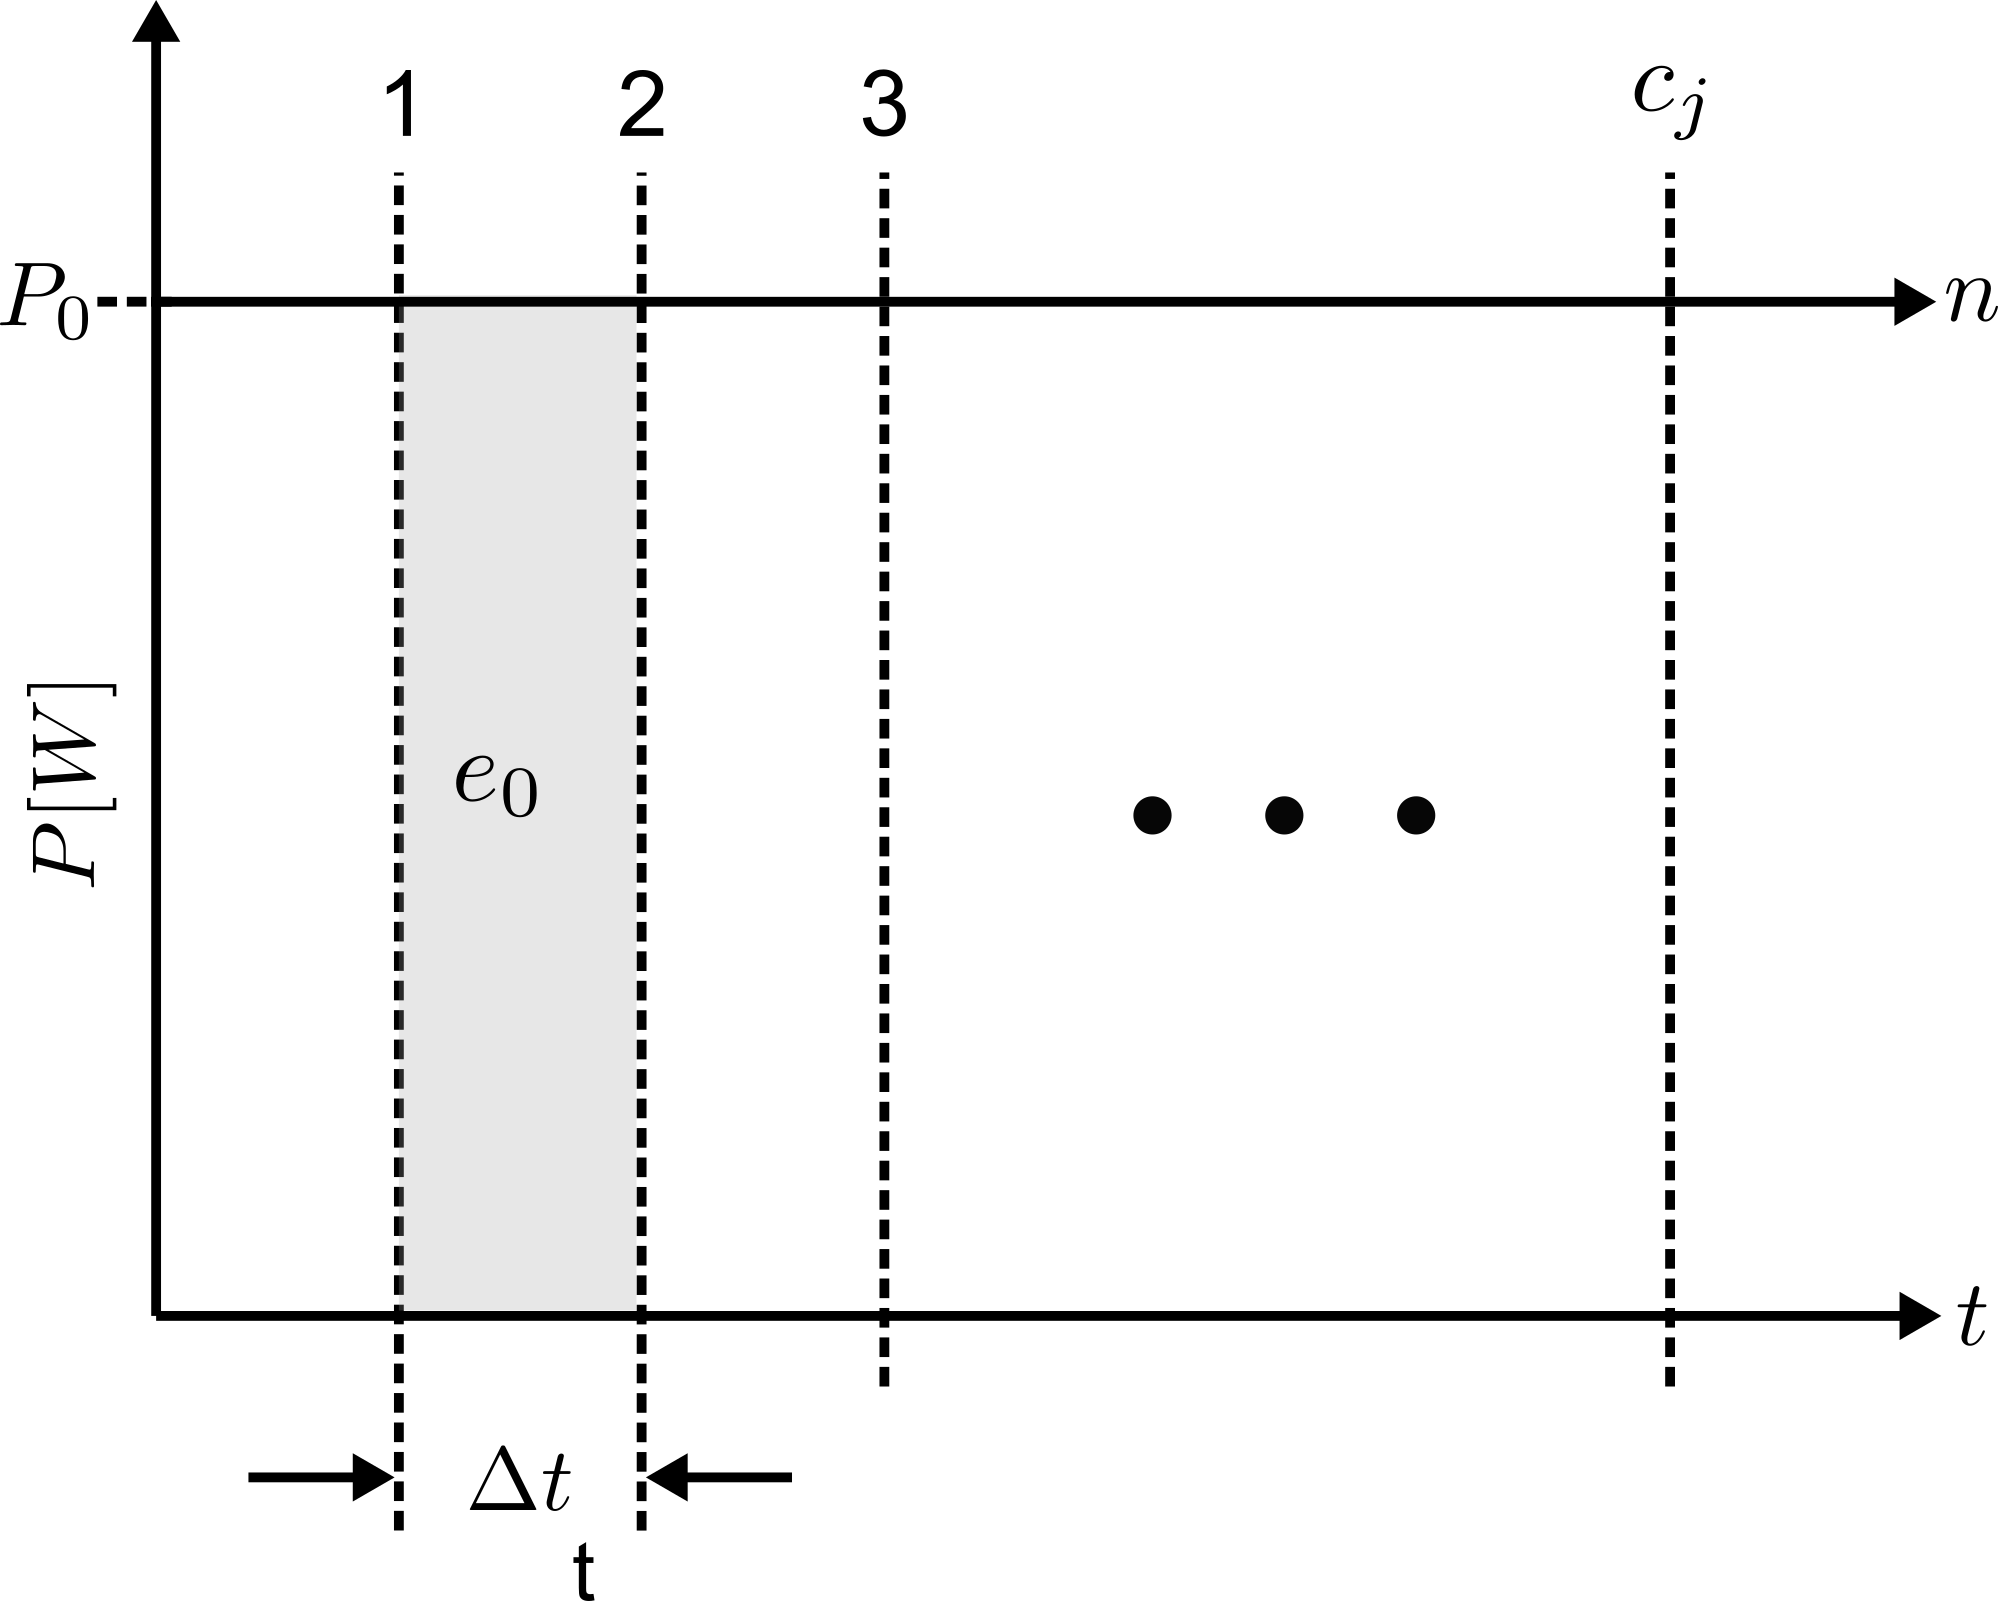
\includegraphics[width=0.45\textwidth]{fig/power_per_episode.png}
	\caption{Power consumption per episode.}
	\label{fig:power_per_episode}
\end{figure}
% ---
\paragraph{Energy requirements.}
Under Asm.~\ref{assumption:power_and_episode_time}, the energy consumption of the $n$-th episode $e_j(n)$ is the constant product
% ---
\begin{equation}\label{eq:energy_per_episode}
	e_j(n) = \underbrace{P_0 \Delta t}_{\text{constant}} = e_0.
\end{equation}
% ---
Consequently, the energy consumed by a robot learning a skill $ s_j $ is directly proportional to the skill complexity $c_j$; i.e.
% ---
\begin{equation}\label{eq:energy_per_skill}
	E_j =\sum_{n=1}^{c_j} e_j(n) = e_0c_j.
\end{equation}
% ---
The energy spent on learning $\mathcal{S}$ under the absence of knowledge transfer is
% ---
\begin{equation}\label{eq:total_energy}
	E_{\mathcal{S}} = \sum_{j=1}^{{N_{\mathcal{S}}}} E_j = e_0 \sum_{j=1}^{{N_{\mathcal{S}}}} c_j%N_{\mathcal{T}} \cdot e_0 \cdot c_j 
\end{equation}
% ---
% ---------------------------------------------------------------------------------------------------
\paragraph{Time requirement.} Similarly, the total learning time $T_{\mathcal{S}}$ for a simple agent is
% ---
\begin{equation}\label{eq:total_time}
	T_{\mathcal{S}} = \Delta t \sum_{j=1}^{{N_{\mathcal{S}}}} c_j.
\end{equation}
% ---

% ===================================================================================================
\subsection{The different learning paradigms}\label{sec:types_of_learning}

% ---------------------------------------------------------------------------------------------------
\paragraph{Isolated Learning (IsL)} A robot performs IsL when it learns each skill in $\mathcal{Z}_k$ one after another from the ground up, disregarding the accumulating knowledge from already learned skills. In such a case the rate of convergence and the initial remaining knowledge for all skills are given by
% ---		
\begin{subequations}\label{eq:fg_isolated}
	\begin{alignat}{2}
		f_{j,k}\left(\cdot \right) &=  -\alpha \\
		g_{j,k}\left(\cdot \right) &= 1,
	\end{alignat}
\end{subequations}
% ---
where $ \alpha>0$ models the rate at which a robot in isolation learns any given skill. Relying on Asm.~\ref{assumption:agent_similarity} we can assign a value to $\alpha$ by using the fundamental complexity $c_0$ as follows
% ---
\begin{equation}\label{eq:isolated_learning_rate}
	\alpha = -\frac{1}{c_0}\text{log}(\epsilon).
\end{equation}
% ---
Since in isolated learning $c^{(IsL)}_{j,k} = c_0$, the trial episodes required by one single robot to learn the skills in the cluster $\mathcal{Z}_k$ is given by
% ---
\begin{equation}
	%	\begin{split}
		%		C^{(IsL)}_{k} &= \sum_{j=1}^{N_{\mathcal{Z}}} c^{(IsL)}_{j,k}= N_{\mathcal{Z}}  \cancelto{c_{0}}{c^{(IsL)}_{j,k}} = N_{\mathcal{Z}} c_0
		%	\end{split}
	C^{(IsL)}_{k} = \sum_{j=1}^{N_{\mathcal{Z}}} c^{(IsL)}_{j,k}= N_{\mathcal{Z}}  c^{(IsL)}_{j,k} = N_{\mathcal{Z}} c_0.
\end{equation}
%-- 
Similarly, the total trial episodes to learn the universe of skills is simply
% ---
\begin{equation}
	C^{(IsL)}_{\mathcal{S}} = N_\mathcal{K} N_{\mathcal{Z}} c_0.
\end{equation}
% ---

\textbf{Multi agent case.} Suppose that a batch of $m$ robots is used to learn the same number of skills in parallel in a given cluster $\mathcal{Z}_k$. Such a strategy only distributes equally the total number of episodes by the number of available robots; i.e.
% ---
\begin{equation}
	^{\lvert \lvert}C^{(IsL)}_k=  \overbrace{\frac{1}{m}C^{(IsL)}_k}^{\text{episodes per robot}}.
\end{equation}
% ---

% ---------------------------------------------------------------------------------------------------
\paragraph{\textbf{Incremental Learning (IL)}}
It corresponds to the continuous aggregation and exchange of knowledge from \emph{intra-cluster} skills. Referring back to Asm.~\ref{assumption:skill_clustering}, the knowledge from skills belonging to a cluster ${\mathcal{Z}_k}$ can be be leveraged by an agent in virtue of their significant similarity. As depicted in Fig.~\ref{fig:intra_skill_learning}, a robot ($r_1$ in this case) learns every skill in $\mathcal{Z}_1$ with a rate $\alpha$ ---the self loops--- but also retains and uses the acquired knowledge to learn subsequent skills. The effect of incremental learning on the knowledge collection rate can be modeled to be directly proportional to the number of learned skills as
% ---
\begin{equation}\label{eq:f_function_incremental}
	f_{j,k}\left(N_{\zeta_k}\right) = -\alpha\left(\eta N_{\zeta_k} + 1 \right), 
\end{equation}
% ---
where $\eta>0$ represents the efficiency of knowledge exchange from $\zeta_k$ to $s_{j,k}$. Different potential models might be used to model the depletion of the initial remaining knowledge represented by $g_{j,k}\left(N_{\zeta_k}\right)$, e.g. a linear decay rate, our expectation is that, under the assumption that a learning strategy involving the ordering of skills according to similarity and their balanced distribution in the different clusters, $g_{j,k}\left(N_{\zeta_k}\right)$ might naturally resemble an exponential decay that is strongly dependent on $N_{\zeta_k}$. Such considerations motivate our choice of the following function
% ---
\begin{equation}\label{eq:g_function_incremental}
	g_{j,k}\left(N_{\zeta_k}\right) = e^{-\delta N_{\zeta_k}},
\end{equation}
%---
again with a factor $\delta>0$ controlling the rate at which the exponential converges. Similar to $\alpha$, using Asm.~\ref{assumption:cluster_size} $\delta$ can be defined as 
% ---
\begin{equation}\label{eq:delta}
	\delta = -\frac{1}{N_\mathcal{Z}}\text{log}(\epsilon).
\end{equation}
% ---
Essentially, such choice of $\delta$ implies that the remaining knowledge in a cluster after seeing all its skills is negligible. Via the exchange factors $(\eta,\delta)$, in incremental learning the knowledge about every new skill gets gradually increased by leveraging previous knowledge, resulting in
% ---
\begin{equation*}\label{eq:remaining_knowledge__IL}
	\bar{\sigma}^{(IL)}_{i,j}(n) = e^{-\alpha  \left(\eta N_{\zeta_k}+1\right) n} e^{-\delta N_{\zeta_k}}.
\end{equation*}
% ---
As the complexity $c_{j,k}$ of a skill can also be interpreted as the number of trial episodes required for the remaining knowledge to go below a threshold $\epsilon$; i.e.
% ---
\begin{equation*}
	\bar{\sigma}^{(IL)}_{i,j}(n) \Big \rvert_{n \ge c^{(IL)}_{j,k}} \leq \epsilon.
\end{equation*}
% ---
Then, under this scheme the complexity $c^{(IL)}_{j,k}$ to learn a new is skill in the cluster results in
% ---
\begin{equation}\label{eq:complexity_IL}
	c^{(IL)}_{j,k} = -\frac{\text{log}(\epsilon) - \text{log}\left(\bar{\sigma}^{(IL)}_{j,k}(0)\right)}{\alpha (\eta N_{\zeta_k}+ 1)} = -\frac{\text{log}(\epsilon) + \delta N_{\zeta_k}}{\alpha (\eta N_{\zeta_k}+ 1)}  .
\end{equation}
% ---
The total number of trial episodes $ C_k $ that an agent following an incremental learning strategy needs to learn the $N_{\mathcal{Z}_k}$ skills in a cluster $ \mathcal{Z}_k $ is given by
% ---
\begin{align}\label{eq:total_episodes_incremental}
	\begin{split}
		C^{(IL)}_k &= \sum^{N_{\mathcal{Z}}}_{j=1} c^{(IL)}_{j,k}.
	\end{split}
\end{align}
% ---

\textbf{Multi-agent case.} If $m$ robots are used in parallel to divide the load of learning the tasks then
% ---
\begin{align}
	\begin{split}
		{}^{\lvert \rvert}C^{(IL)}_k &= \sum^{\frac{N_{\mathcal{Z}}}{m}}_{j=1} c^{(IL)}_{j,k}.
	\end{split}
\end{align}
% --
In essence, using $m$ robots without exchanging knowledge only subdivides the learning in every cluster into $m$ smaller problems \emph{without adding any additional benefit to the rate at which knowledge is acquired}. 

% ---------------------------------------------------------------------------------------------------
\paragraph{\textbf{Transfer + Incremental Learning (TIL)}}
Transfer learning (TL) alone refers to the one-time \emph{inter-cluster} exchange of knowledge. Considering $\mathcal{K} = \{ \mathcal{Z}_k \}^{N_\mathcal{K}}_{k=1}$ to be the set of all available skill clusters, TL represents the exchange of knowledge from the skills learned in different \emph{origin} clusters $\mathcal{O} = \{ \mathcal{Z}_1,\mathcal{Z}_2,\ldots,\mathcal{Z}_{k-1} \}$ to the skills that will be learned in a \emph{destination} cluster $\mathcal{Z}_k$ (see Fig.~\ref{fig:cluster_to_cluster_knowledge_transfer_parallel}). Concretely, the effect that TL has on the skills of the destination cluster is the reduction of the initial remaining knowledge and the increase of the initial learning rate for all the skills in the $k$-th cluster via the parameter $\beta_k$; i.e.
% ---
\begin{equation}\label{eq:f_function_transfer}
	f_{j,k}\left(N_{\zeta_k}\right) = -\alpha \left( \frac{\eta N_{\zeta_k} + 1}{1 - \beta_k} \right),
\end{equation}
% ---
and
% ---
\begin{equation}\label{eq:g_function_transfer}
	g_{j,k}\left(N_{\zeta_k}\right) = (1-\beta_k) e^{-\delta N_{\zeta_k}}.
\end{equation}
%---
In essence, $\beta_k$ is the head start granted by knowledge transfer from other clusters to the skills in $\mathcal{Z}_k$. We argue that  $0<\beta_{k} < 1$ since it represents the \emph{aggregated} knowledge exchange factor from the different origin clusters $\mathcal{Z}_{c}$ to the target cluster $\mathcal{Z}_{k}$. Let $0<\beta_{c} < 1$ be the transfer contribution factor of a single origin cluster $\mathcal{Z}_c$. Additionally, consider that
% ---
\begin{equation}
	\sum\limits_{c=1}^{N_\mathcal{K}}\beta_{c} \leq 1,
\end{equation}
% --
as $1$ represents all the knowledge in $\mathcal{S}$. Asm.~\ref{assumption:cluster_transferability} implies that $\beta_c$ is equal for all the clusters. In this work we select $\beta_c = 1/N_\mathcal{K}$ for simplicity. The aggregated transfer factor $\beta_k$ is the sum of the individual factors from the already-visited clusters; i.e.
% ---
\begin{equation}\label{eq:beta_k_transfer}
	\beta_{k}= \left(k-1\right)\beta_c = \left(k-1\right)\frac{1}{N_\mathcal{K}}.
\end{equation}
% ---

Consequently, the remaining knowledge when transfer and incremental learning are used in conjunction is
% ---
\begin{equation}\label{eq:remaining_knowledge__ITL}
	\bar{\sigma}^{(TIL)}_{j,k}(n) = \left(1- \beta_k\right) e^{-\alpha  \left(\frac{ \eta N_{\zeta_k}+1}{1 - \beta_k}\right) n} e^{-\delta N_{\zeta_k}}.
\end{equation}
% ---
Similar to incremental learning, the complexity to learn a skill in transfer learning is
\begin{equation}\label{eq:skill_complexity_TL}
	c^{(TIL)}_{j,k} = -\frac{1 - \beta_{k}}{\alpha (\eta N_{\zeta_k}+ 1)}\left[\text{log}(\epsilon) + \delta N_{\zeta_k} - \text{log}(1 - \beta_{k})\right]
\end{equation}
% ---
and the total number of episodes  $ C_k $ that an agent requires to learn the $N_{\mathcal{Z}_k}$ skills is merely their sum
% ---
\begin{align}\label{eq:total_episodes_transfer}
	\begin{split}
		C^{(TIL)}_k &= \sum^{N_{\mathcal{Z}}}_{j=1} c^{(TIL)}_{j,k}.
	\end{split}
\end{align}
% --- 

\textbf{Multi-agent case.} If $m$ robots are used in parallel to divide the load of learning the tasks then, the transfer of knowledge from cluster to cluster is also divided by the number of robots, this implies that \eqref{eq:beta_k_transfer} changes to
% ---
\begin{equation}\label{eq:beta_k_transfer_parallel}
	{}^{\lvert \rvert}\beta_{k}= \frac{1}{m}\beta_{k}.
\end{equation}
% ---
Correspondingly, when using transfer learning in parallel $\beta_k$ is replaced by ${}^{\lvert \rvert}\beta_{k}$ in \eqref{eq:skill_complexity_TL}. Then, similar to IL, the total number of episodes to learn the skills in a cluster is
% ---
\begin{align}
	\begin{split}
		{}^{\lvert \rvert}C^{(TIL)}_k &= \sum^{\frac{N_{\mathcal{Z}}}{m}}_{j=1} c^{(TIL)}_{j,k}.
	\end{split}
\end{align}
% ---
This case is depicted on Fig.~\ref{fig:cluster_to_cluster_knowledge_transfer_parallel}, where two robots $ r_1$ and $r_2$ learn skills in four different clusters. The shaded areas are the subclusters of skills learned by each robot. Since they do not share knowledge between them, each robot has access only to the knowledge it has collected and cannot benefit from one another. 

% ---------------------------------------------------------------------------------------------------
%\subsection*{\textbf{Collective learning (CL)}}
%As mentioned in Sec.~\ref{sec:intro}, EAI agents will be a core element of industrial, healthcare, and domestic ecosystems with advanced communication and remote processing capabilities. Given the anticipated legions of EAI agents executing and learning several different skills at any given time in those environments, it is immediately evident that the previous learning paradigms are not meant to exploit these large number of agents together with the advanced communication and processing infrastructure to take full advantage of the potential for concurrent knowledge exchange among the agents. Therefore, the use of isolated, incremental, and transfer learning by these many agents 
%would directly aggravate computational demand (see challenge C1). As discussed in \cite{Kaelbling2020foundationefficientrobot} an leaning algorithm that would allow an agent to learn new tasks on-the-fly would need to be sample-efficient, generalizable, compositional, and (truly) incremental. Collective learning is the natural paradigm that meets this requirements exploiting the full communication potential of the networked EAI agents to leverage the real-time synergistic exchange and aggregation of collected knowledge to make the learning of tasks energy- and time-efficient.
%
%To formalize this idea, let $ \left\lbrace \rho_i \right\rbrace_{i=1}^{m} $ be a set of robotic agents that defines a community of robots. In collective learning, the different robotic agents $ \rho_i $ develop and accumulate dynamically a common mind (body of knowledge) via networked interactions where individual experience, knowledge and skills are disseminated to all the other elements in the collective. Information flows vertically as previous knowledge is passed on, as well as horizontally by sharing concurrent experience between agents. Via these mechanisms, knowledge can be replicated, complimented and further developed. We take from \cite{Garavan2012CollectiveLearning} two notions central in collective learning that are applicable to the embodied AI agents:
%% ---
%\begin{enumerate}
%	\item Capability to restructure and meet changing conditions
%	\item Aggregation of skills, knowledge, and behaviors
%\end{enumerate}
%% ---
%Collective learning contrasts with the previously discussed incremental learning in that a single agent $ r_i $ can aggregate only so much knowledge via trial and error and is limited by a sequential learning structure. Learning collectively, on the other hand, enforces parallelization of knowledge acquisition via the concurrent learning and sharing of all agents as they acquire new skills, knowledge. Moreover, collective learning involves not only the information acquisition, but also how this information is brought to use to form and develop knowledge. 
%
%CL is not only a promising research direction but, in our opinion, has the potential to be a unifying solution to the grand challenges posed by embodied AI. Furthermore, by incorporating new mechanical designs as elements of the learning pipeline it is possible to iteratively evaluate the energy efficiency of proposed solutions and select the best ones as reference designs for future manufacturing processes with underlying learning, therefore, promoting a cyclical optimization towards a semi-optimal general design.
%
%Unlike isolated and transfer learning, in this paradigm a batch of robots $\left \lbrace r_i \right \rbrace^m_{1}$ not only learn different skills concurrently but also exchange the acquired knowledge between each other and are actually able to leverage it. To enable CL, it is assumed that
%\begin{itemize}
%	\item an inter-agent communication protocol/infrastructure is in place that
%	\item enables agents to concurrently exchange and integrate the self-acquired and received knowledge to
%	\item incrementally speed up the learning of all the agents as a whole.
%\end{itemize}
%% ---
%As a result, the intra- and inter-cluster knowledge transfer is possible. Naturally, the CL paradigm involves a complex scheduling problem to determine the optimal skill distribution and inter-agent knowledge sharing strategy. Since we have not tackled this problem yet, we ground the subsequent discussion on Assumptions~\ref{assumption:average_behavior}, \ref{assumption:agent_similarity},~\ref{assumption:cluster_size}, and~\ref{assumption:cluster_transferability} that suggest an average behavior given a suitable scheduling.
%
%Fig.~\ref{fig:cl_example_figure} illustrates the CL concept, where the self loop represents the dynamics of a single robot learning (at a rate $\alpha$). The exchange of knowledge across agents is represented via the cross-couplings weighted by a parameter $\gamma$ that models how efficient is the bidirectional pairwise knowledge exchange. Similar to transfer learning, if two robots exchange knowledge about skills with low similarity (i.e. skills in different clusters), then $\gamma$ is scaled by the inter-cluster transferability parameter $\beta$. In CL \eqref{eq:simple_knowledge_dynamics} is extended to 
%% ---
%\begin{subequations}\label{eq:collective_knowledge_dynamics}
%	\begin{empheq}[left=\empheqlbrace]{align}
%		\dot{\bar{\bm{\sigma}}}^{(CL)}_{j,k}\left(n\right) &= \left[  f_{j,k}\left(N_{\zeta_k},r\right) \bm{I} + \gamma \bm{A} \odot \bm{B}  \right] \bar{\bm{\sigma}}^{(CL)}_{j,k}\left(n\right)\\
%		\bar{\bm{\sigma}}^{(CL)}_{j,k}(0) &= g_{j,k}\left( N_{\zeta_k}, r\right) \bm{I},
%	\end{empheq}
%\end{subequations}
%% ---
%where $r=m$ is the number of robots that exchange knowledge among them. This implies that now $\bar{\bm{\sigma}}^{}_{j,k} \in \mathbb{R}^r$ is a vector that represents the dynamics of the remaining knowledge of all the $m$ skills being concurrently learned. $\bm{A} \in \mathbb{R}^{r \times r}$ is a zero-diagonal symmetric adjacency matrix whose entry $(\bm{A})_{i,j} = 1$ if robot $i$ exchanges knowledge with robot $j$ and $(\bm{A})_{i,j} = 0$ if it does not. The term $\gamma \in \mathbb{R}_+ $ weighs the knowledge exchange strength among robots. Furthermore, since there may be robots learning skills in different clusters at the same time, the matrix $\bm{B}$, whose entries are $\left(\bm{B}\right)_{i,j} \in \left \lbrace 1, \beta_{k} \right \rbrace$, with
%% ---
%\begin{equation}
%	%\beta_{k} = 1/N_\mathcal{K}, 
%	\beta_{k} = r\frac{ N_{\zeta_k}}{N_\mathcal{S}}, 
%\end{equation}
%% ---
%scales down the knowledge contributions between robots from different clusters. Finally, the operator $\odot$ represents the Hadamard product of matrices. The functions $ f(\cdot)$ and $g(\cdot)$ are now also dependent on the number of robots that exchange knowledge, which directly impacts the number of skills that enter $\zeta_k$ after a learning cycle; i.e.
%% ---
%\begin{equation}\label{eq:f_function_collective}
%	f_{j,k}\left(N_{\zeta_k},r\right) = -\alpha \left( \frac{\eta r N_{\zeta_k} + 1}{1 - \beta_k} \right),
%\end{equation}
%% ---
%and
%% ---
%\begin{equation}\label{eq:g_function_collective}
%	g_{j,k}\left(N_{\zeta_k},r\right) = (1-\beta_k) e^{-\delta r N_{\zeta_k}}.
%\end{equation}
%%---
%Some considerations need to be taken when selecting the value of $\gamma$ given that the dynamics matrix of the collective system
%% ---
%\begin{equation}
%	\bar{\bm{A}}\left(N_{\zeta_k}\right) = f\left(N_{\zeta_k},r\right) \bm{I} + \gamma \bm{A} \odot \bm{B} 
%\end{equation} 
%% ---
%exhibits a dependency on the number of seen skills $N_{\zeta_k}$, which is directly influenced by the number of robots $r$ in the collective. Yet, it can be proven that there is a coupling strength $\gamma$ for a given connectivity $\bm{A}$ that ensures that the remaining knowledge for all skills converges asymptotically to zero.


% ===================================================================================================
%                                                 |                                                 |
%                                                 |                                                 |
% -------------------------------------------- SECTION ---------------------------------------------|
%                                                 |                                                 |
%                                                 |                                                 |
% ===================================================================================================
\newpage
\section{Results}\label{sec:use_case_results}
Fig.~\ref{fig:collective_learning} shows the results of applying isolated learning, incremental learning, transfer and incremental learning, and collective learning to the learning scenario defined by the tuple
% ---
\begin{equation*}
	\phi_{SF} = \left(N_\mathcal{S}= 512, N_\mathcal{K}=4, m=32, \left[\alpha =  0.0461, \delta =  0.0360, \eta= 0.1\right]\right).
\end{equation*}
% ---
In this scenario all $m$ agents are always concurrently learning skills from the same cluster $Z_i$.
% ---
\begin{figure}[!h]
	\centering
	\hspace*{\fill}
	\subfloat[]{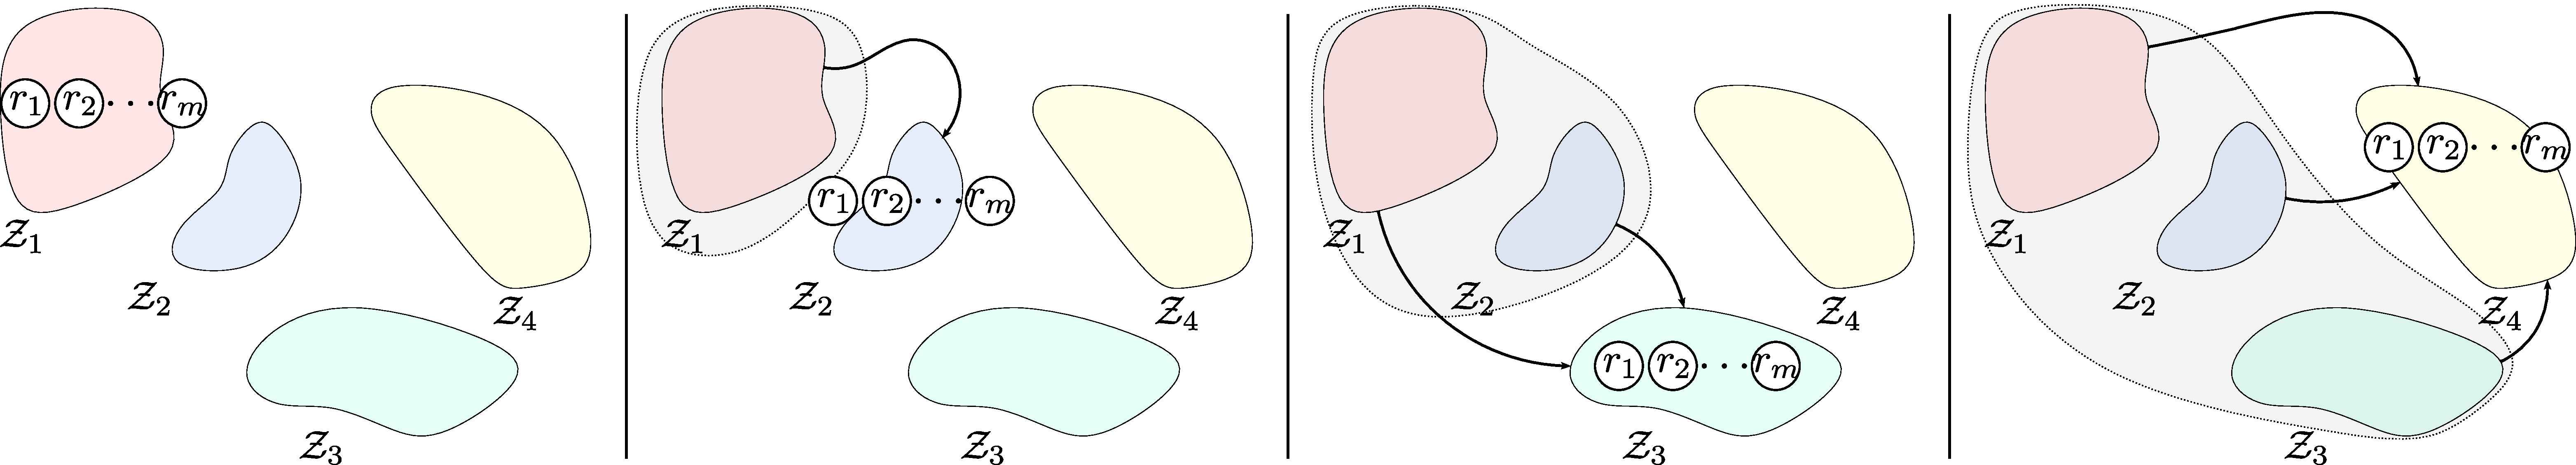
\includegraphics[width= 0.7\textwidth]{fig/cluster_learning_sequence.png} \label{fig:cluster_learning_sequence}}
	\hspace*{\fill}
	\\	
	\hspace*{\fill}
	\subfloat[]{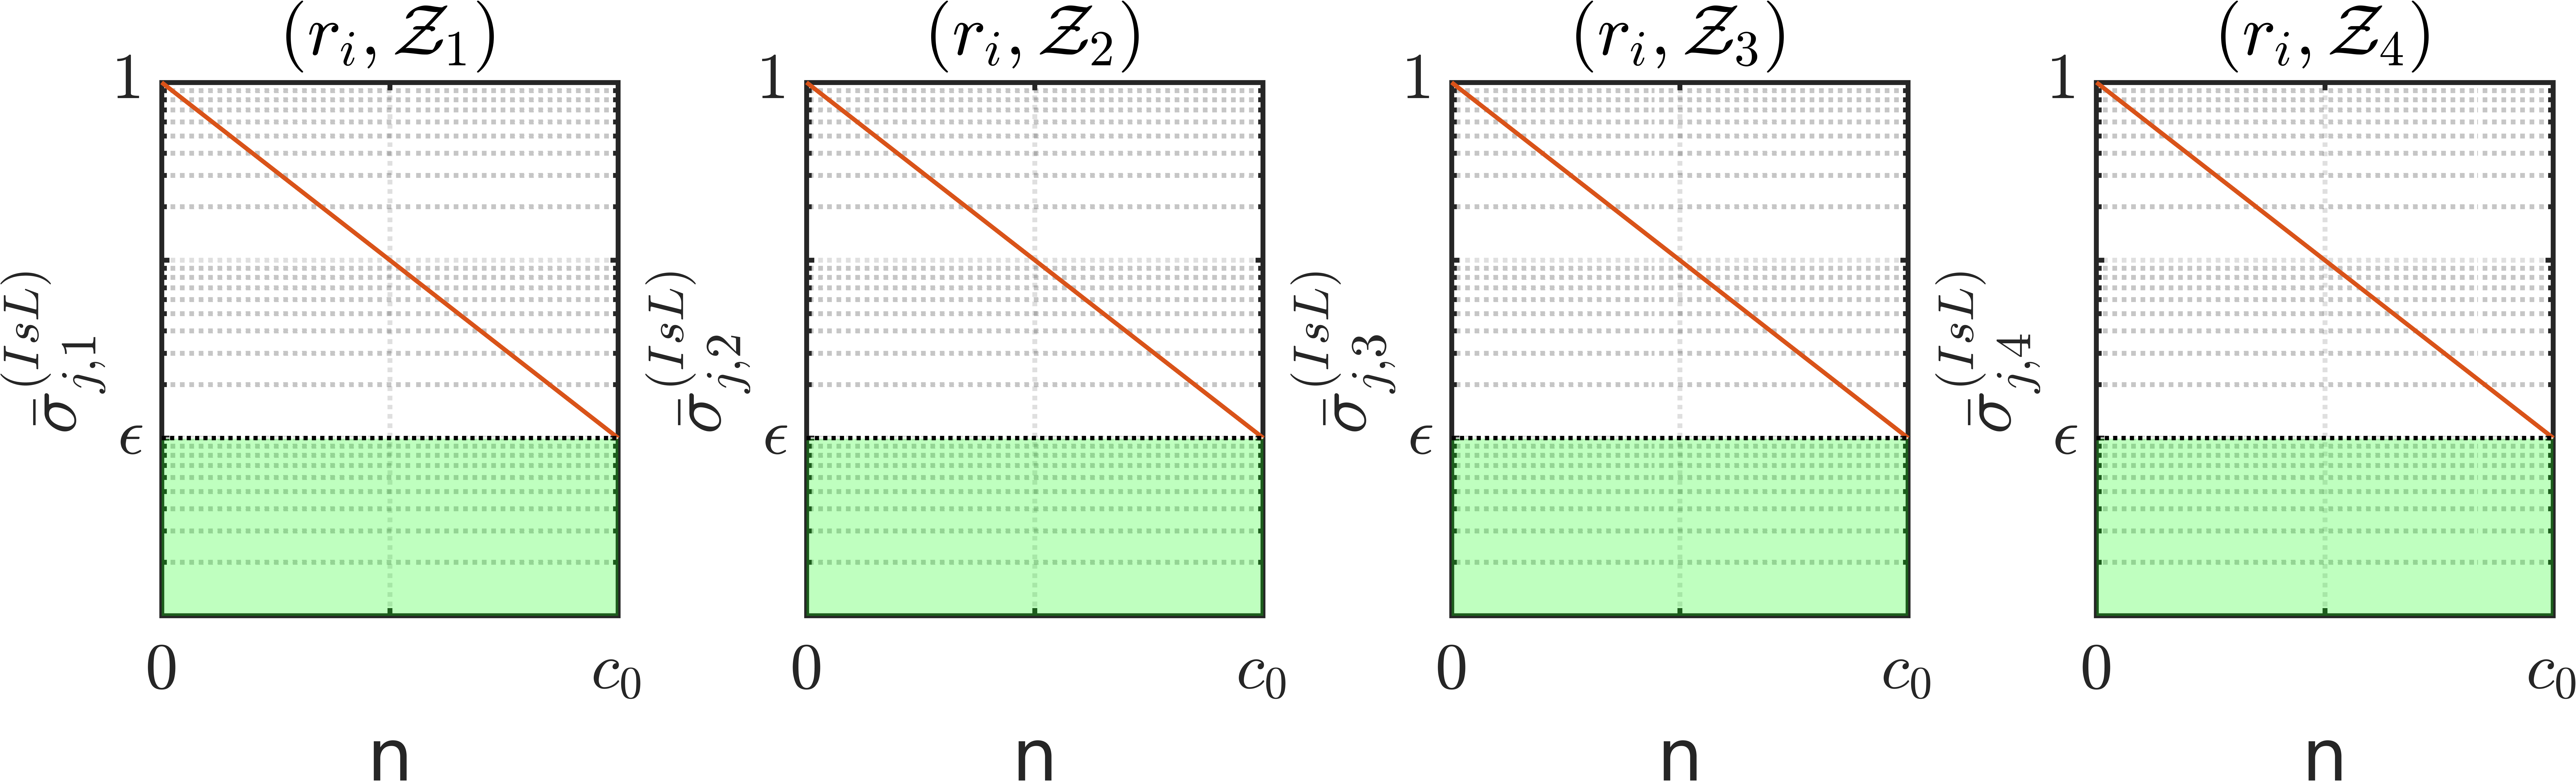
\includegraphics[width= 0.7\textwidth]{fig/dynamics_isolated_learning.png} \label{fig:dynamics_isolated_learning}}  
	\hspace*{\fill}
	\\	
	\hspace*{\fill}
	\subfloat[]{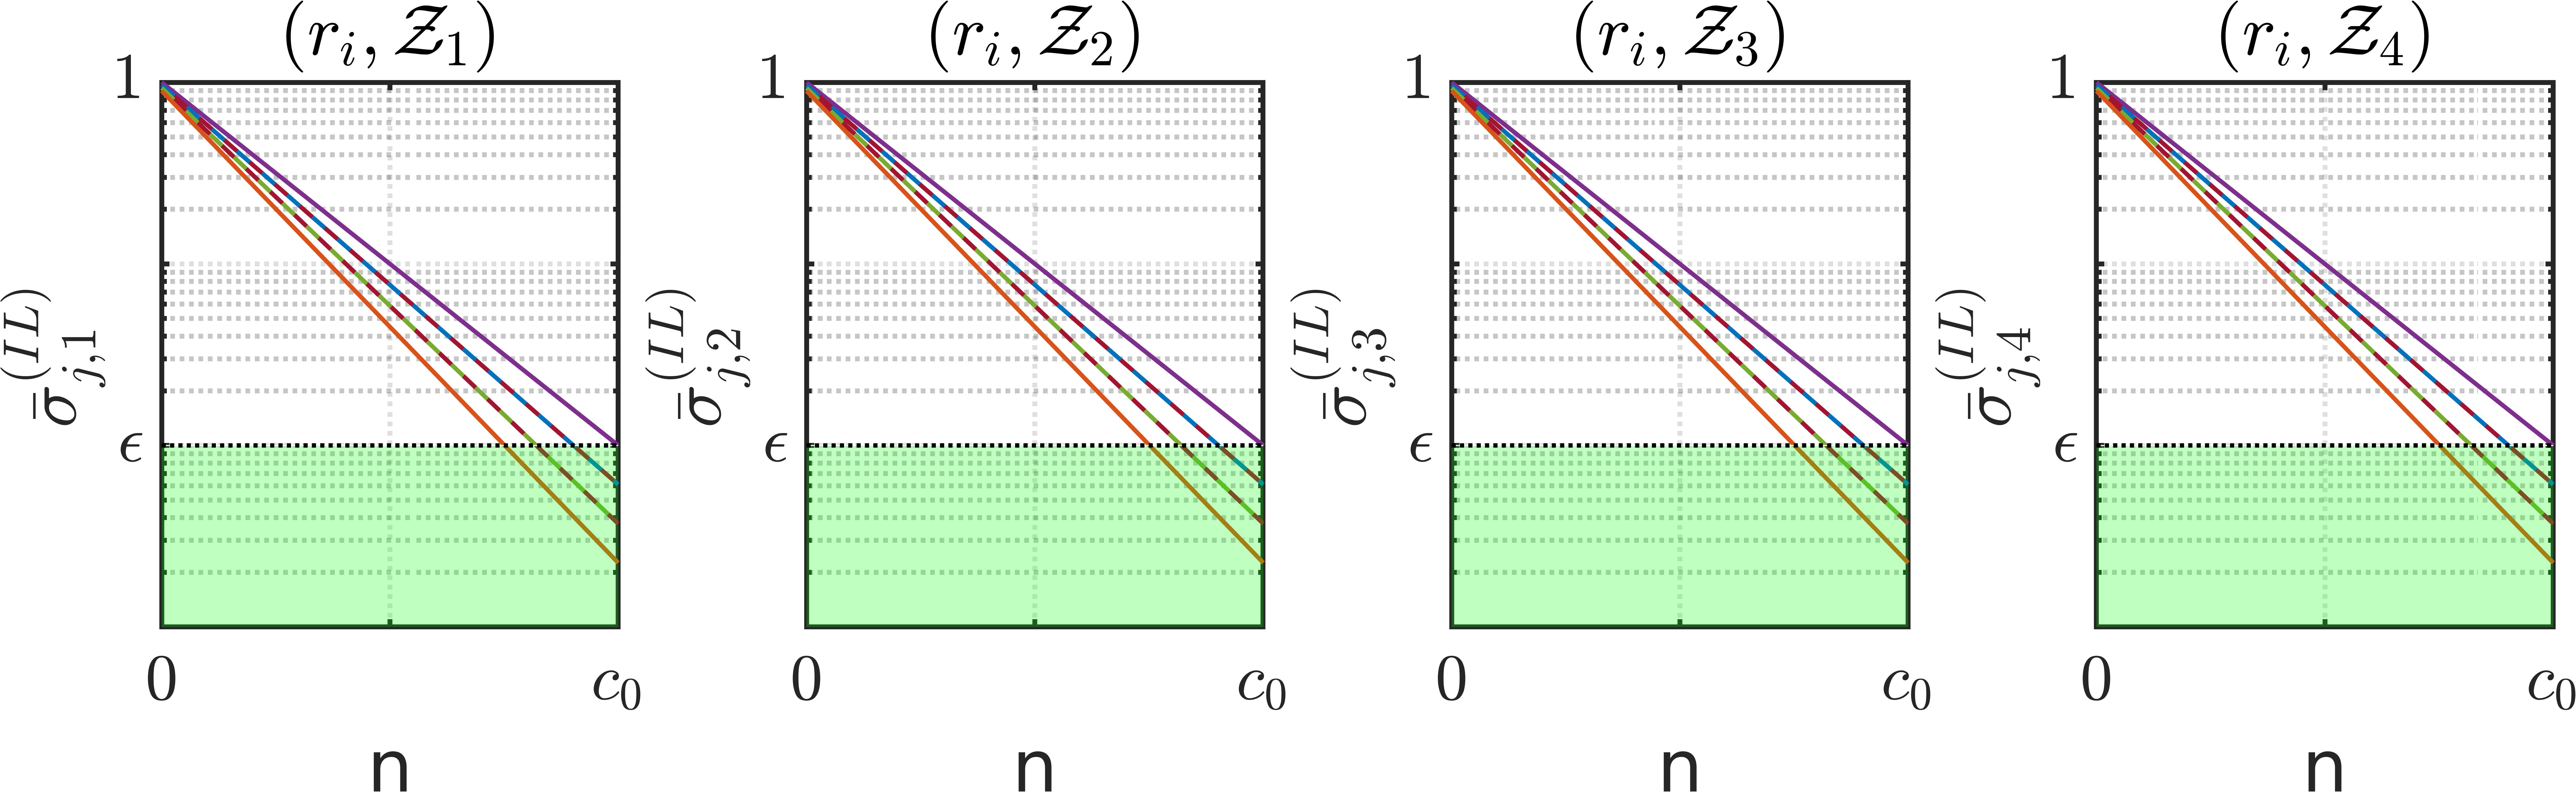
\includegraphics[width= 0.7\textwidth]{fig/dynamics_incremental_learning.png} \label{fig:dynamics_incremental_learning}}  
	\hspace*{\fill}	
	\\
	\hspace*{\fill}
	\subfloat[]{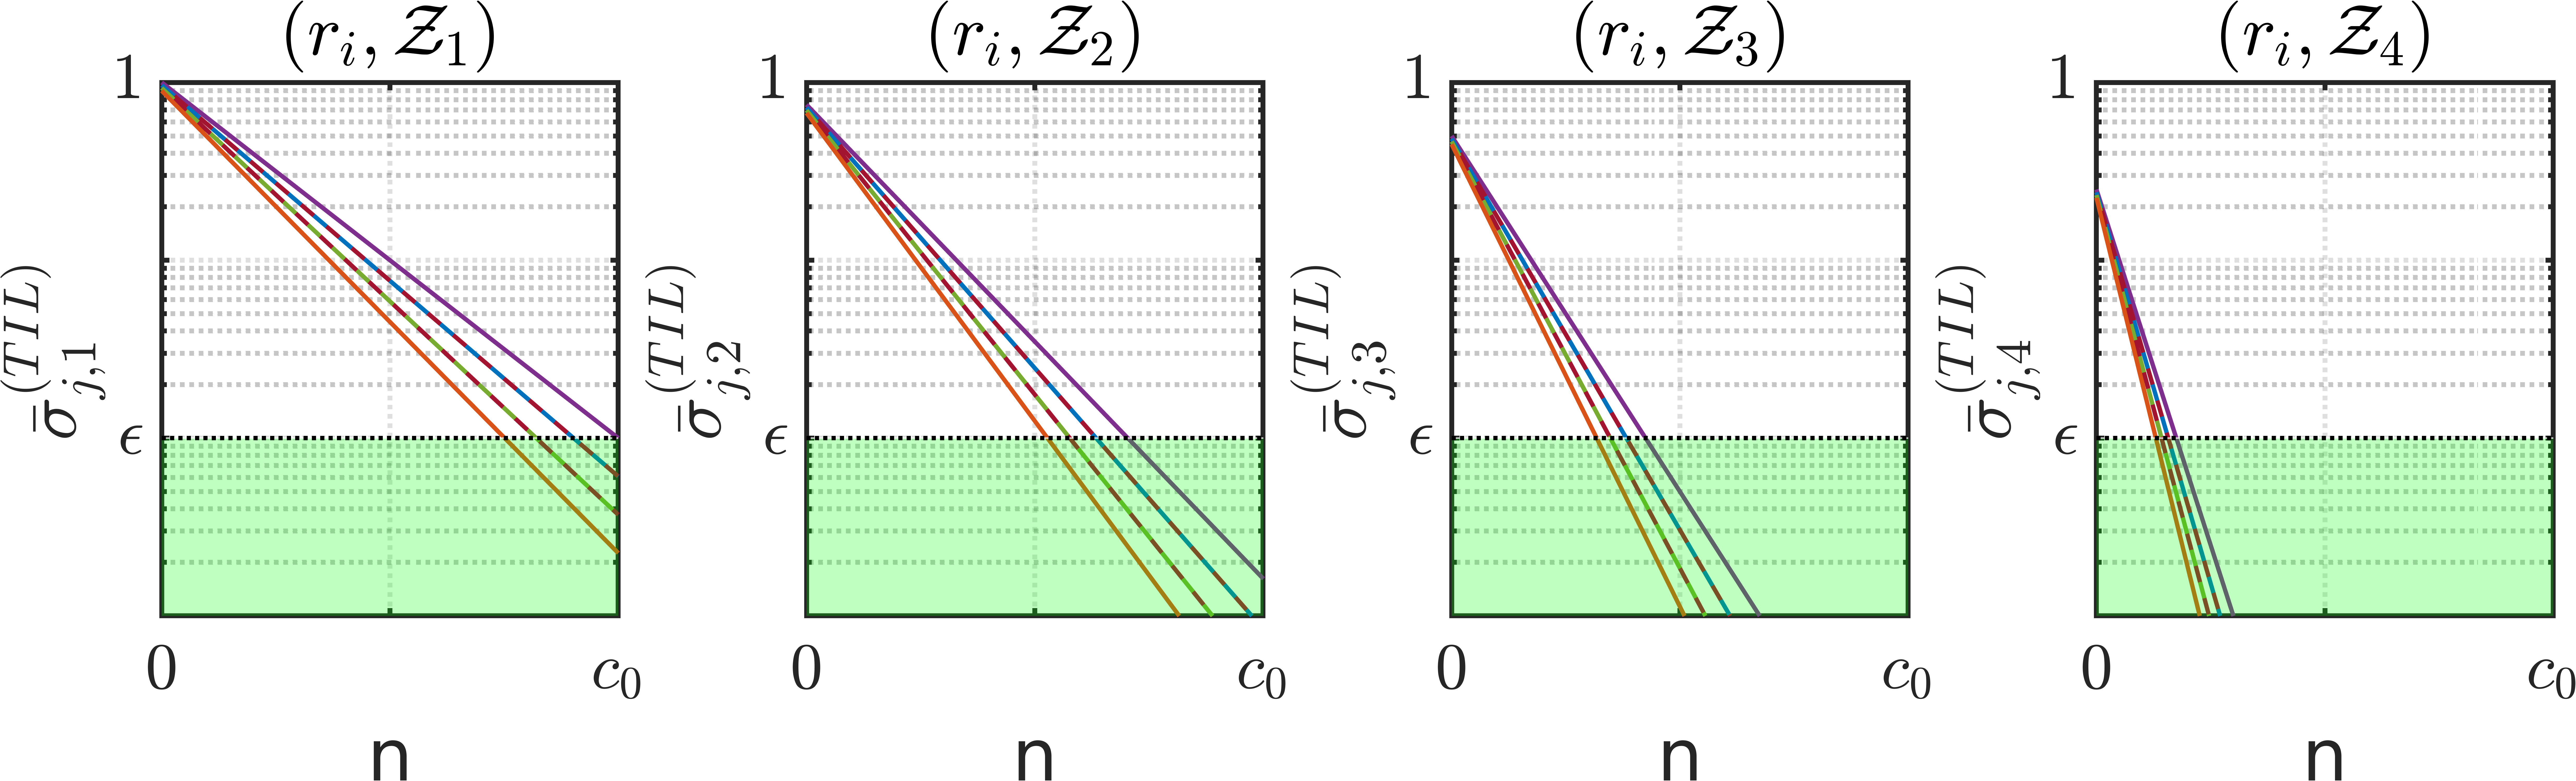
\includegraphics[width= 0.7\textwidth]{fig/dynamics_incremental_transfer_learning.png} \label{fig:dynamics_incremental_transfer_learning}}  
	\hspace*{\fill}
	\\
	\hspace*{\fill}
	\subfloat[]{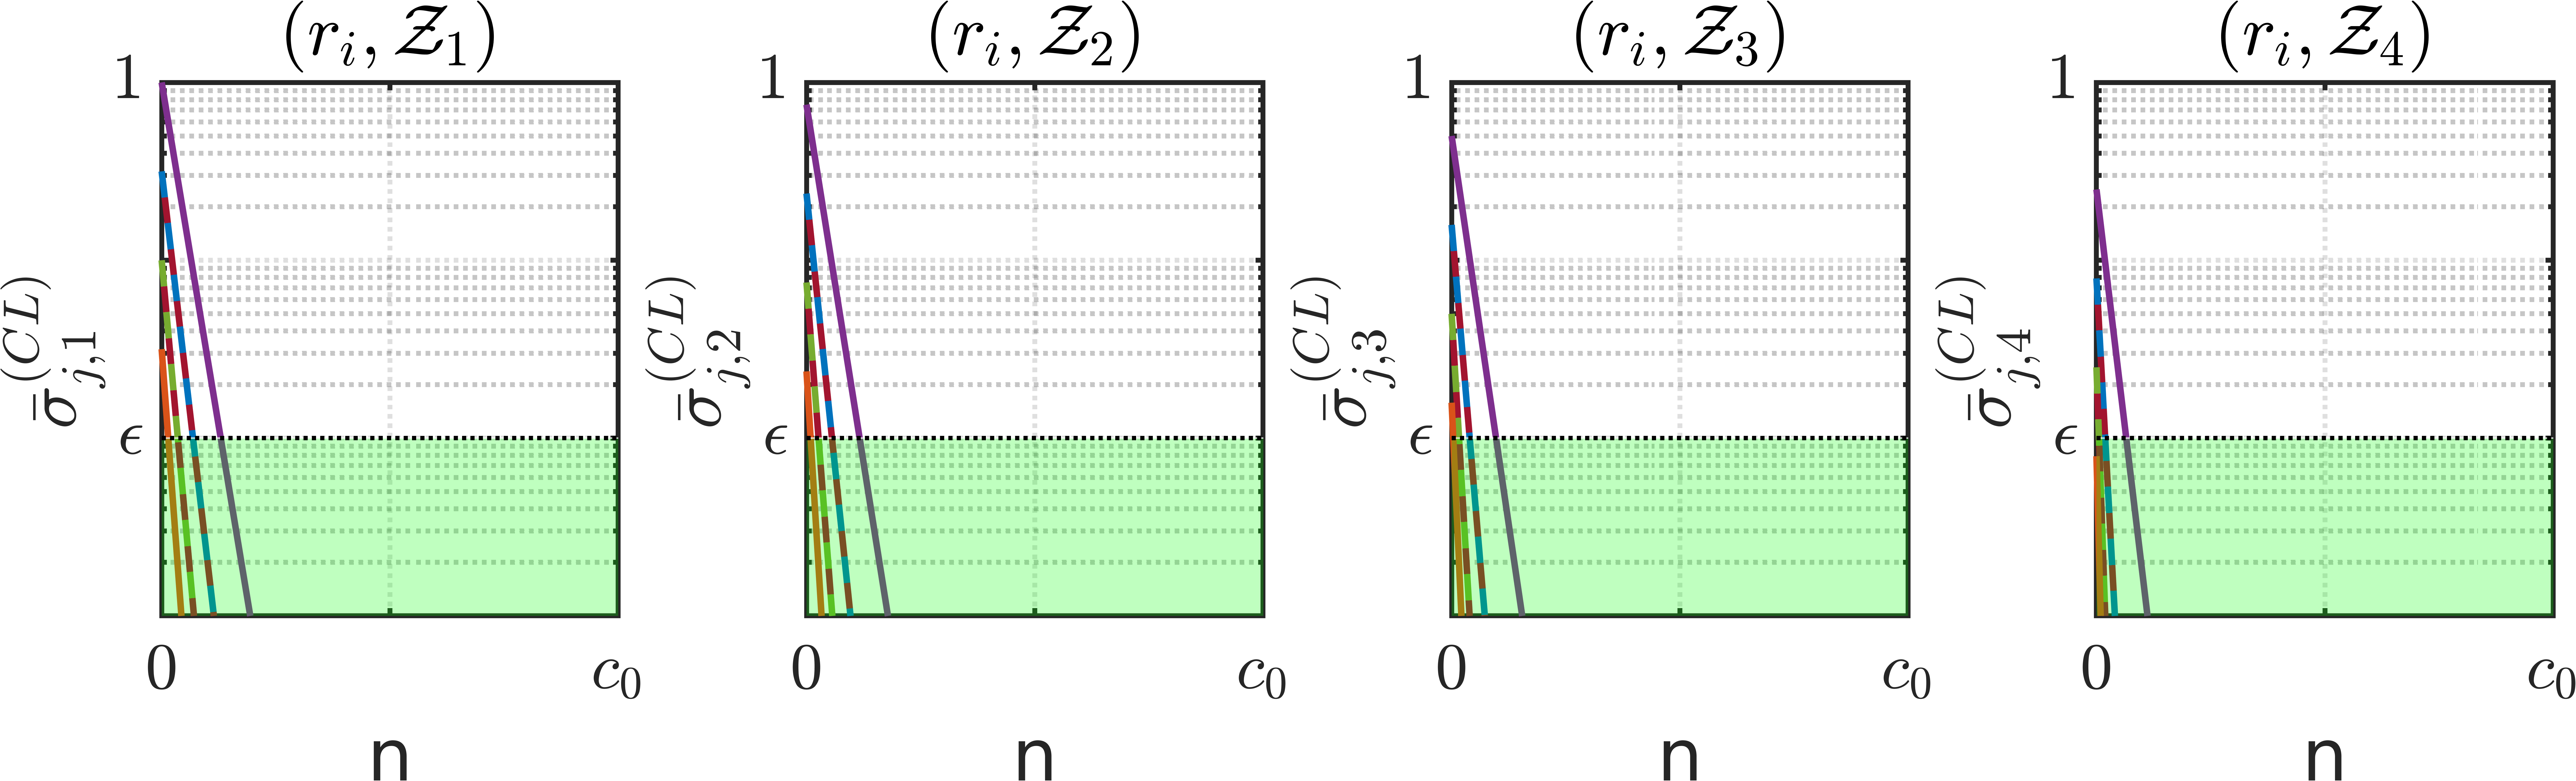
\includegraphics[width= 0.7\textwidth]{fig/dynamics_collective_learning.png} \label{fig:dynamics_collective_learning}}
	\hspace*{\fill}
	\caption[] {\label{fig:collective_learning} Scenario 1: \subref{fig:cluster_learning_sequence} the skills of each cluster are learned by the $ m$ robots in succession, \subref{fig:dynamics_isolated_learning} isolated learning, \subref{fig:dynamics_incremental_learning} incremental learning,  \subref{fig:dynamics_incremental_transfer_learning} incremental + transfer learning, \subref{fig:dynamics_collective_learning} collective learning.}
\end{figure}
% ---


% ===================================================================================================
%                                                 |                                                 |
%                                                 |                                                 |
% -------------------------------------------- SECTION ---------------------------------------------|
%                                                 |                                                 |
%                                                 |                                                 |
% ===================================================================================================
\newpage
\section{Supporting statistics}
% ===================================================================================================
\subsection{Industrial and cobot statistics}\label{sec:robot_statistics}
According to the International Federation of Robotics (IFR) the unit sales of collaborative robots in relation to conventional industrial robots has been constantly increasing in the past years \cite{statista_ir_cobot_share}. Recent data, see Fig.~\ref{fig:industrial_cobot_share}, shows that cobots now make almost 15 \% of the sales.
%---
\begin{figure}[!h]
	\centering
	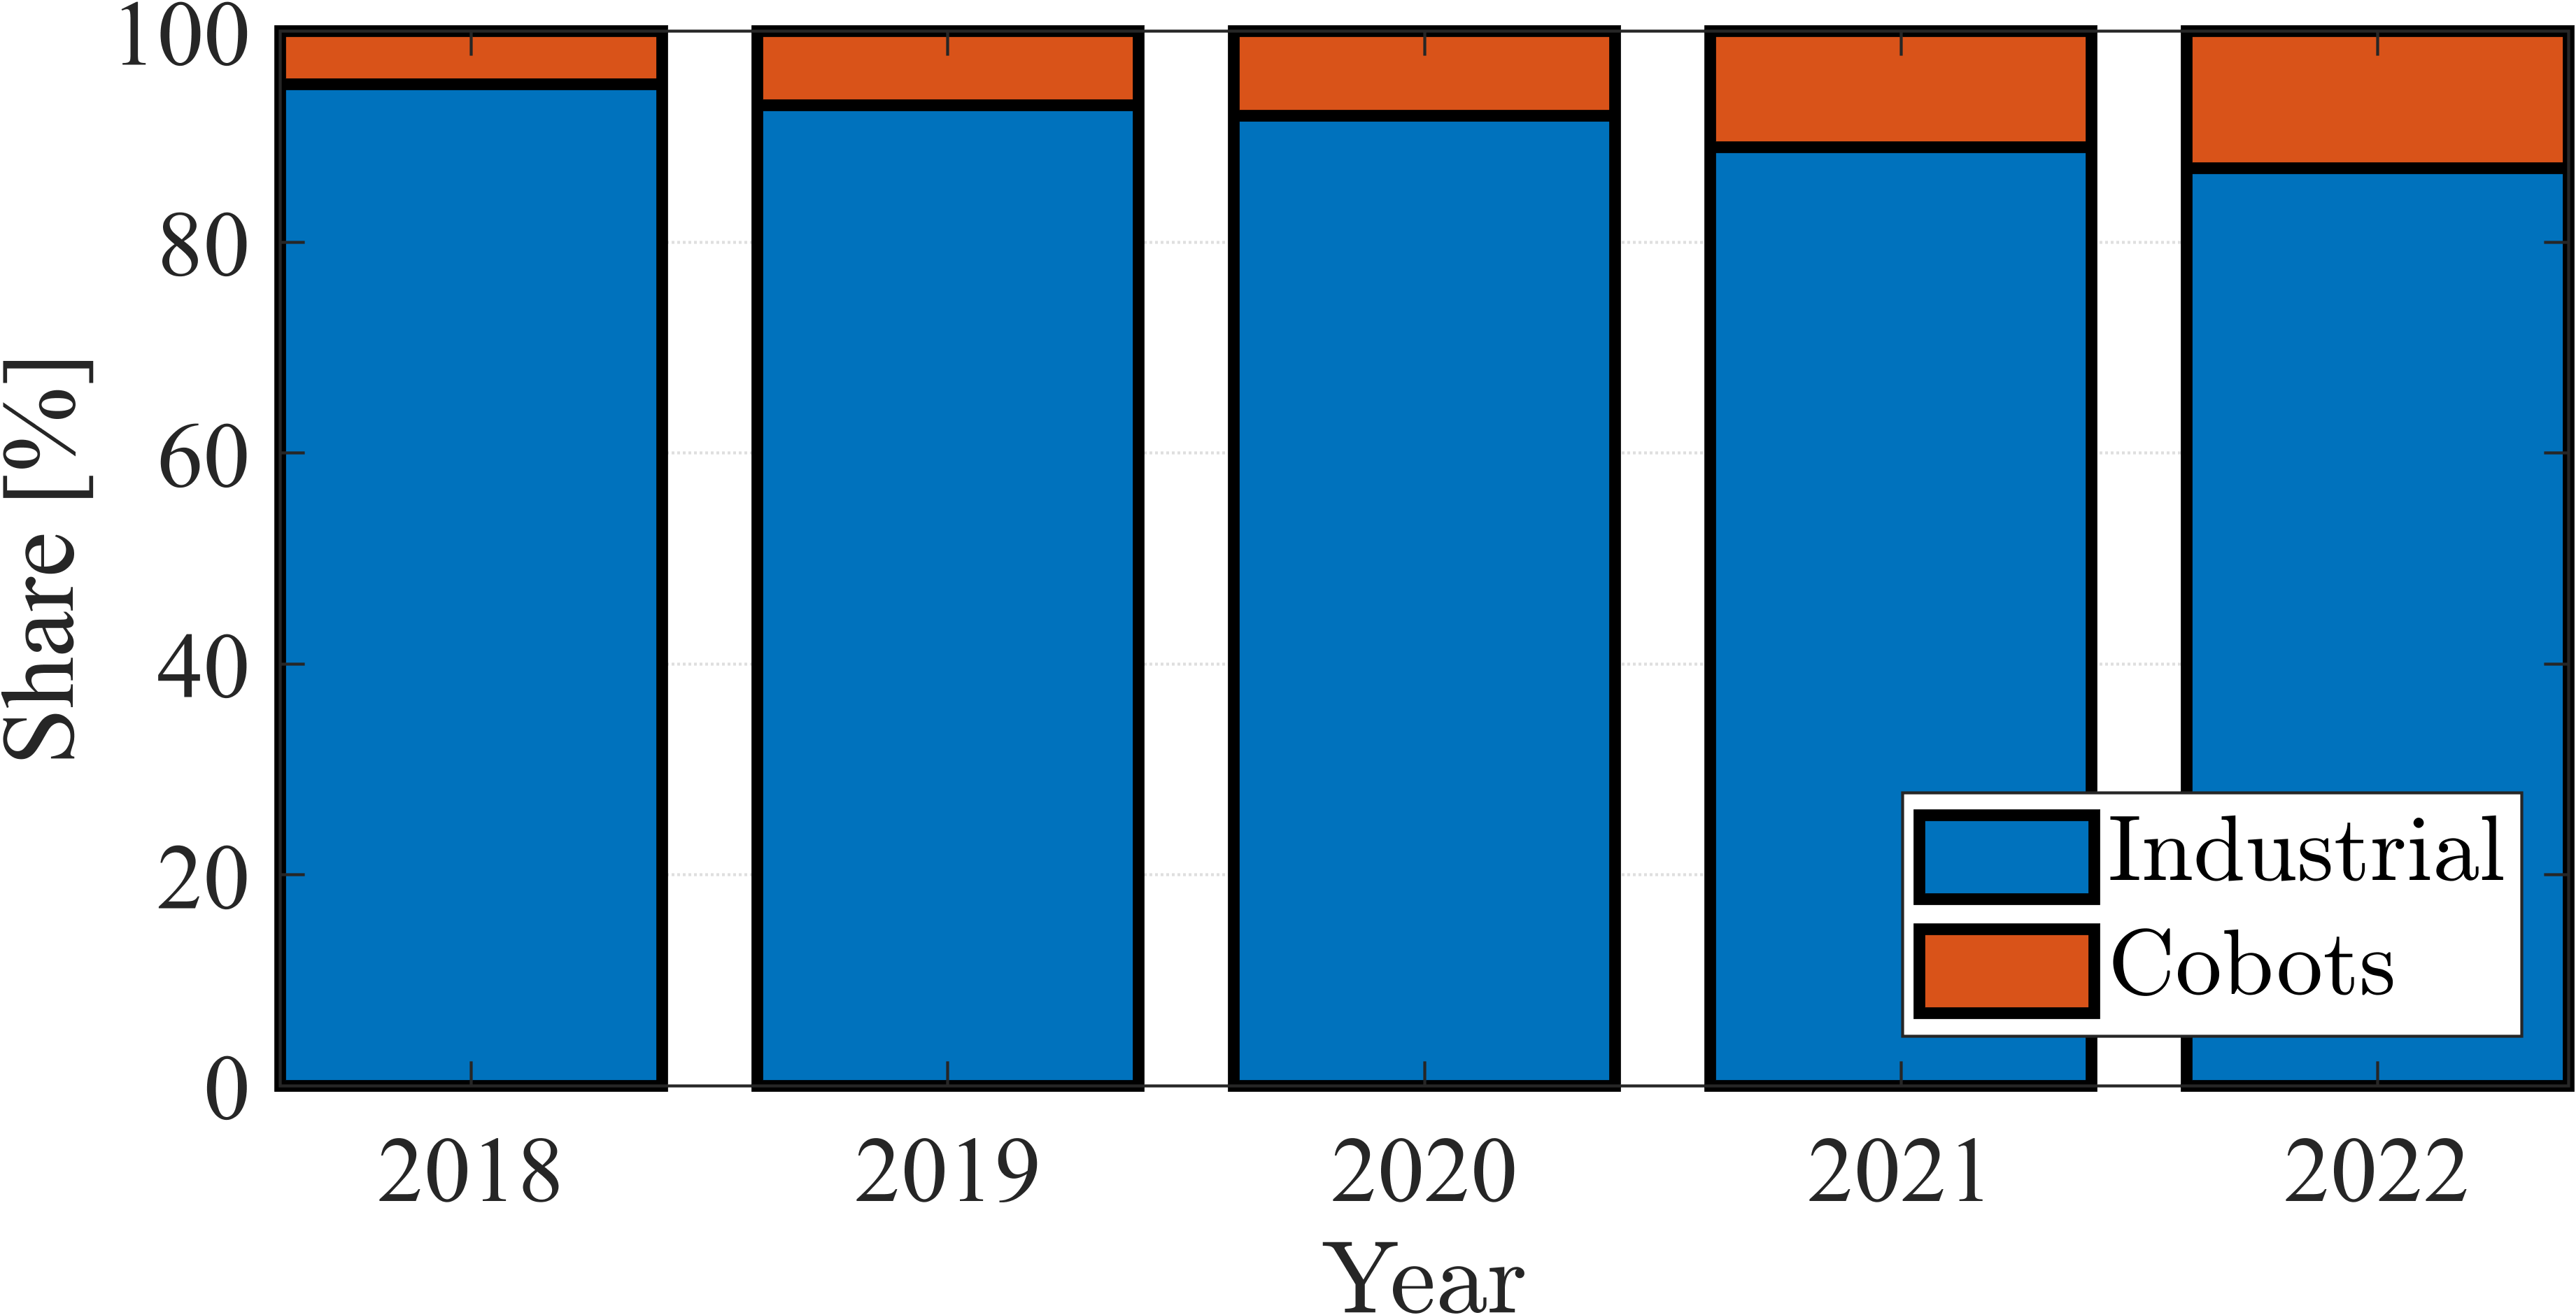
\includegraphics[width= 0.45\textwidth]{fig/share_industrial_and_cobots.png} 
	\caption{Unit sales share industrial robots to cobots }
	\label{fig:industrial_cobot_share}
\end{figure}
% ---

The unit sales are congruent with the the estimated operational stock of industrial (Fig.~\ref{fig:ir_stock}) robots and cobots (\ref{fig:cobot_stock}).
% ---
\begin{figure*}[!h]
	\centering
	\hspace*{\fill}
	\begin{subfigure}[t]{0.45\textwidth}
		\subcaption{}
		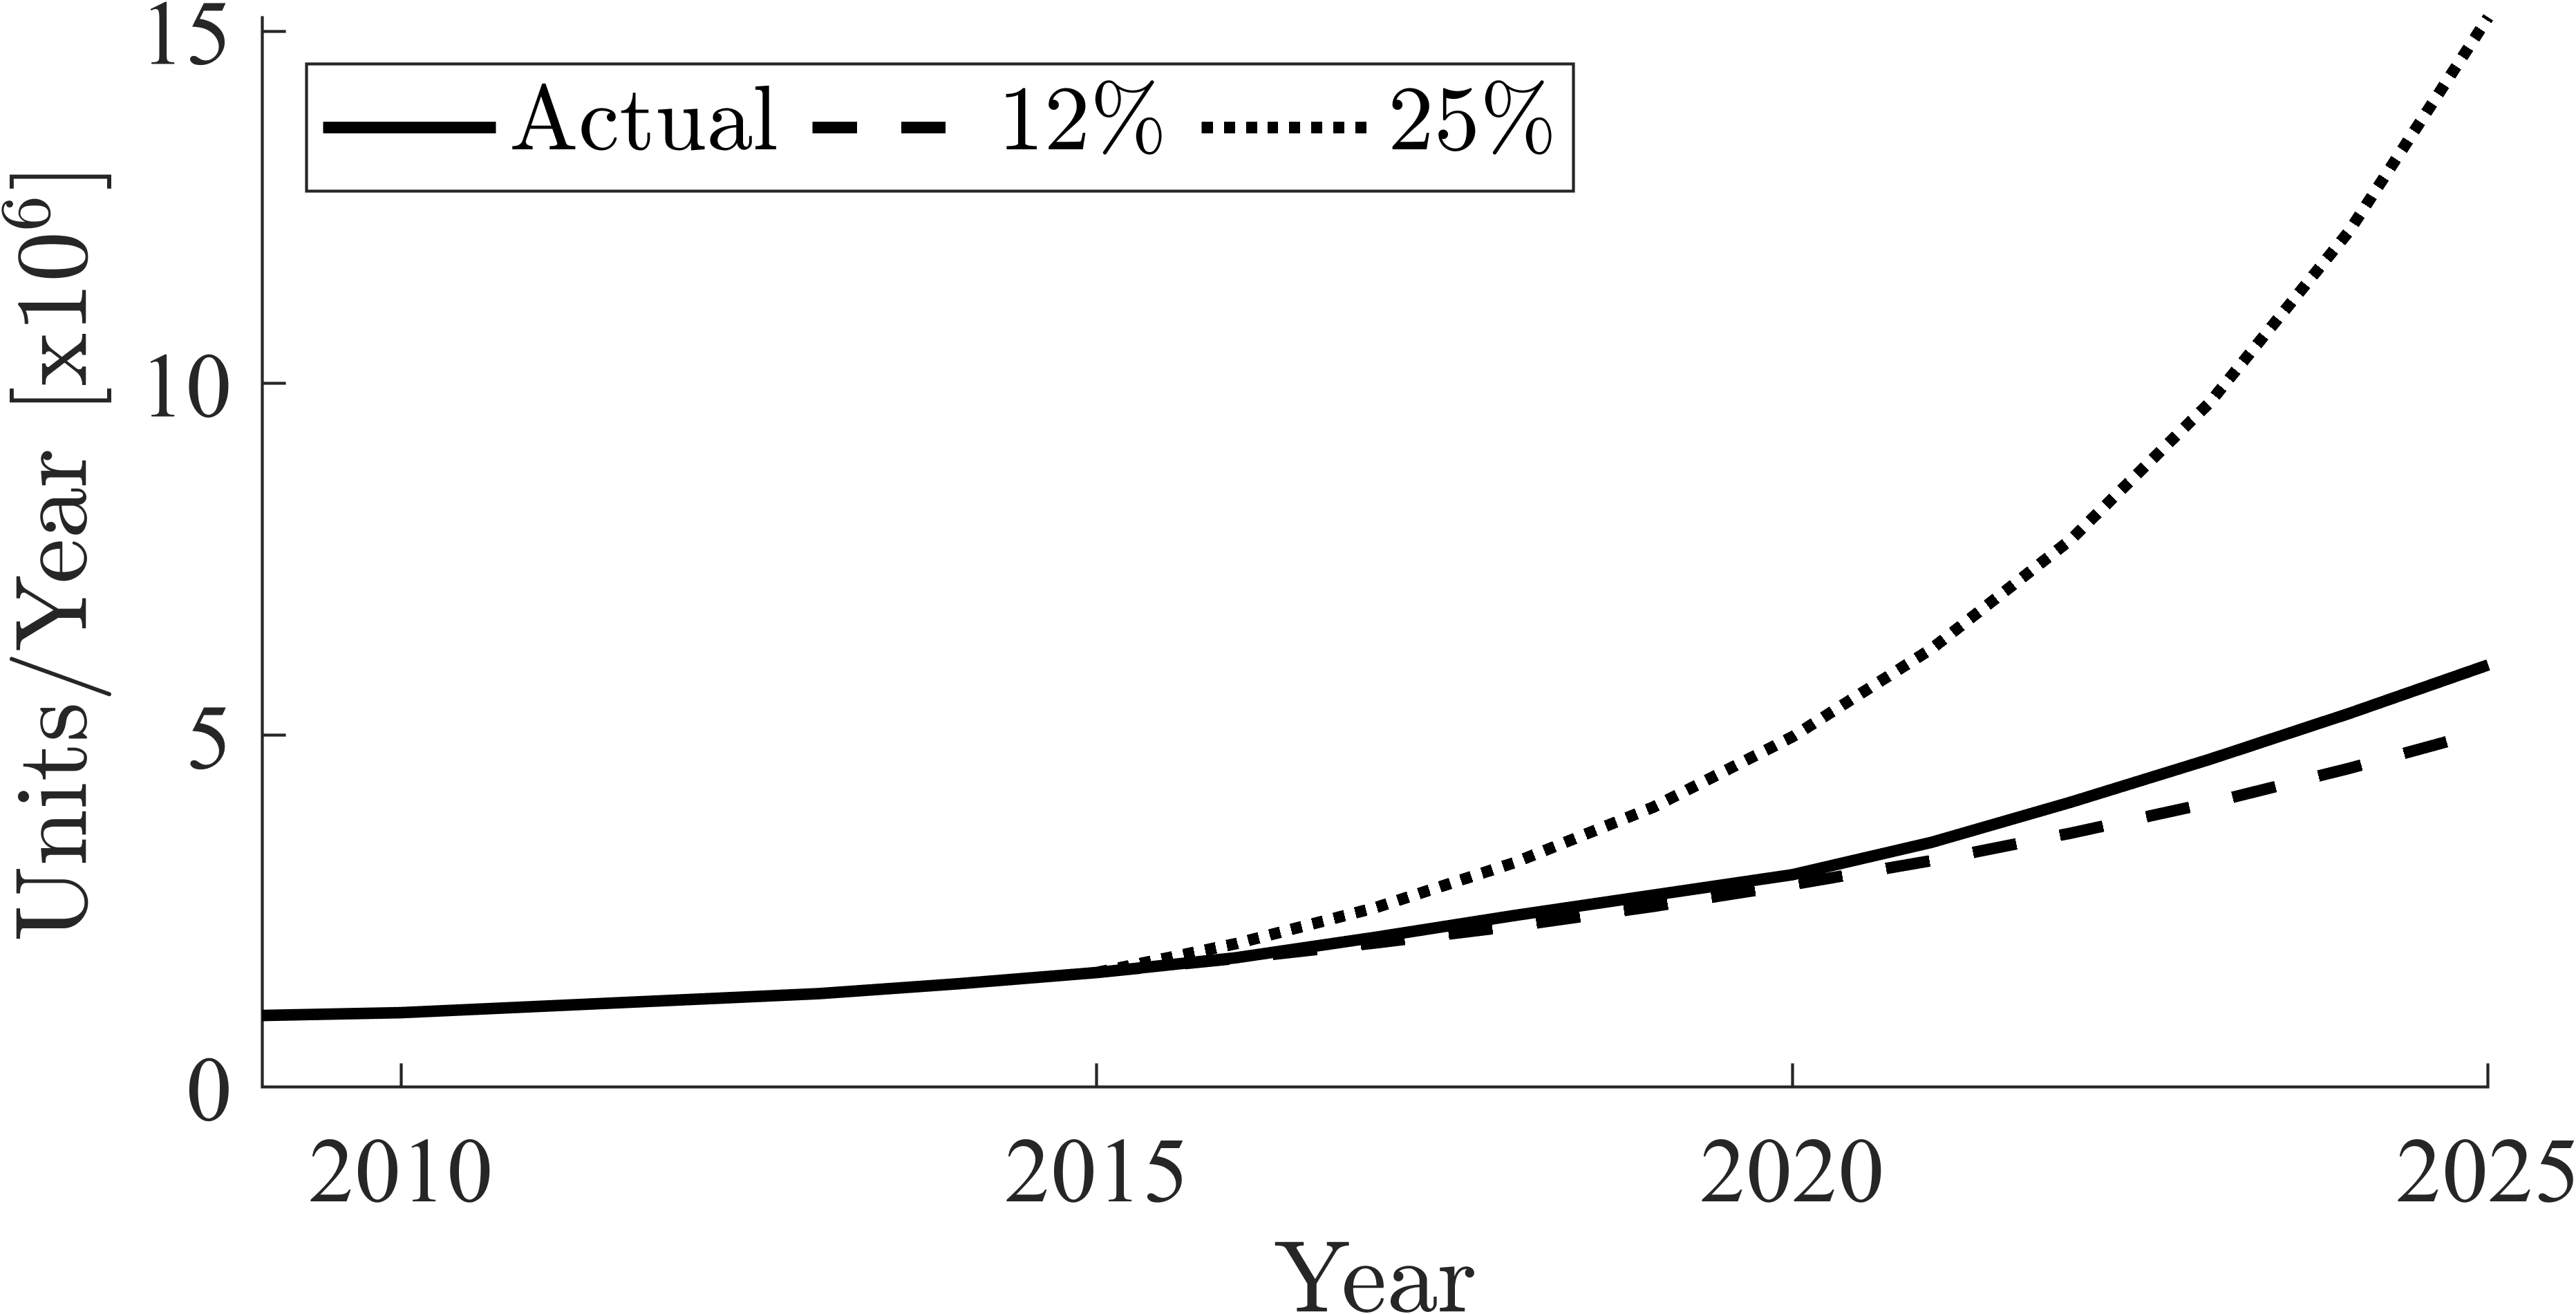
\includegraphics[width= \textwidth]{ir_units_projections.png}
		\label{fig:ir_stock}
	\end{subfigure}
	\hfill
	\begin{subfigure}[t]{0.45\textwidth}
		\subcaption{}
		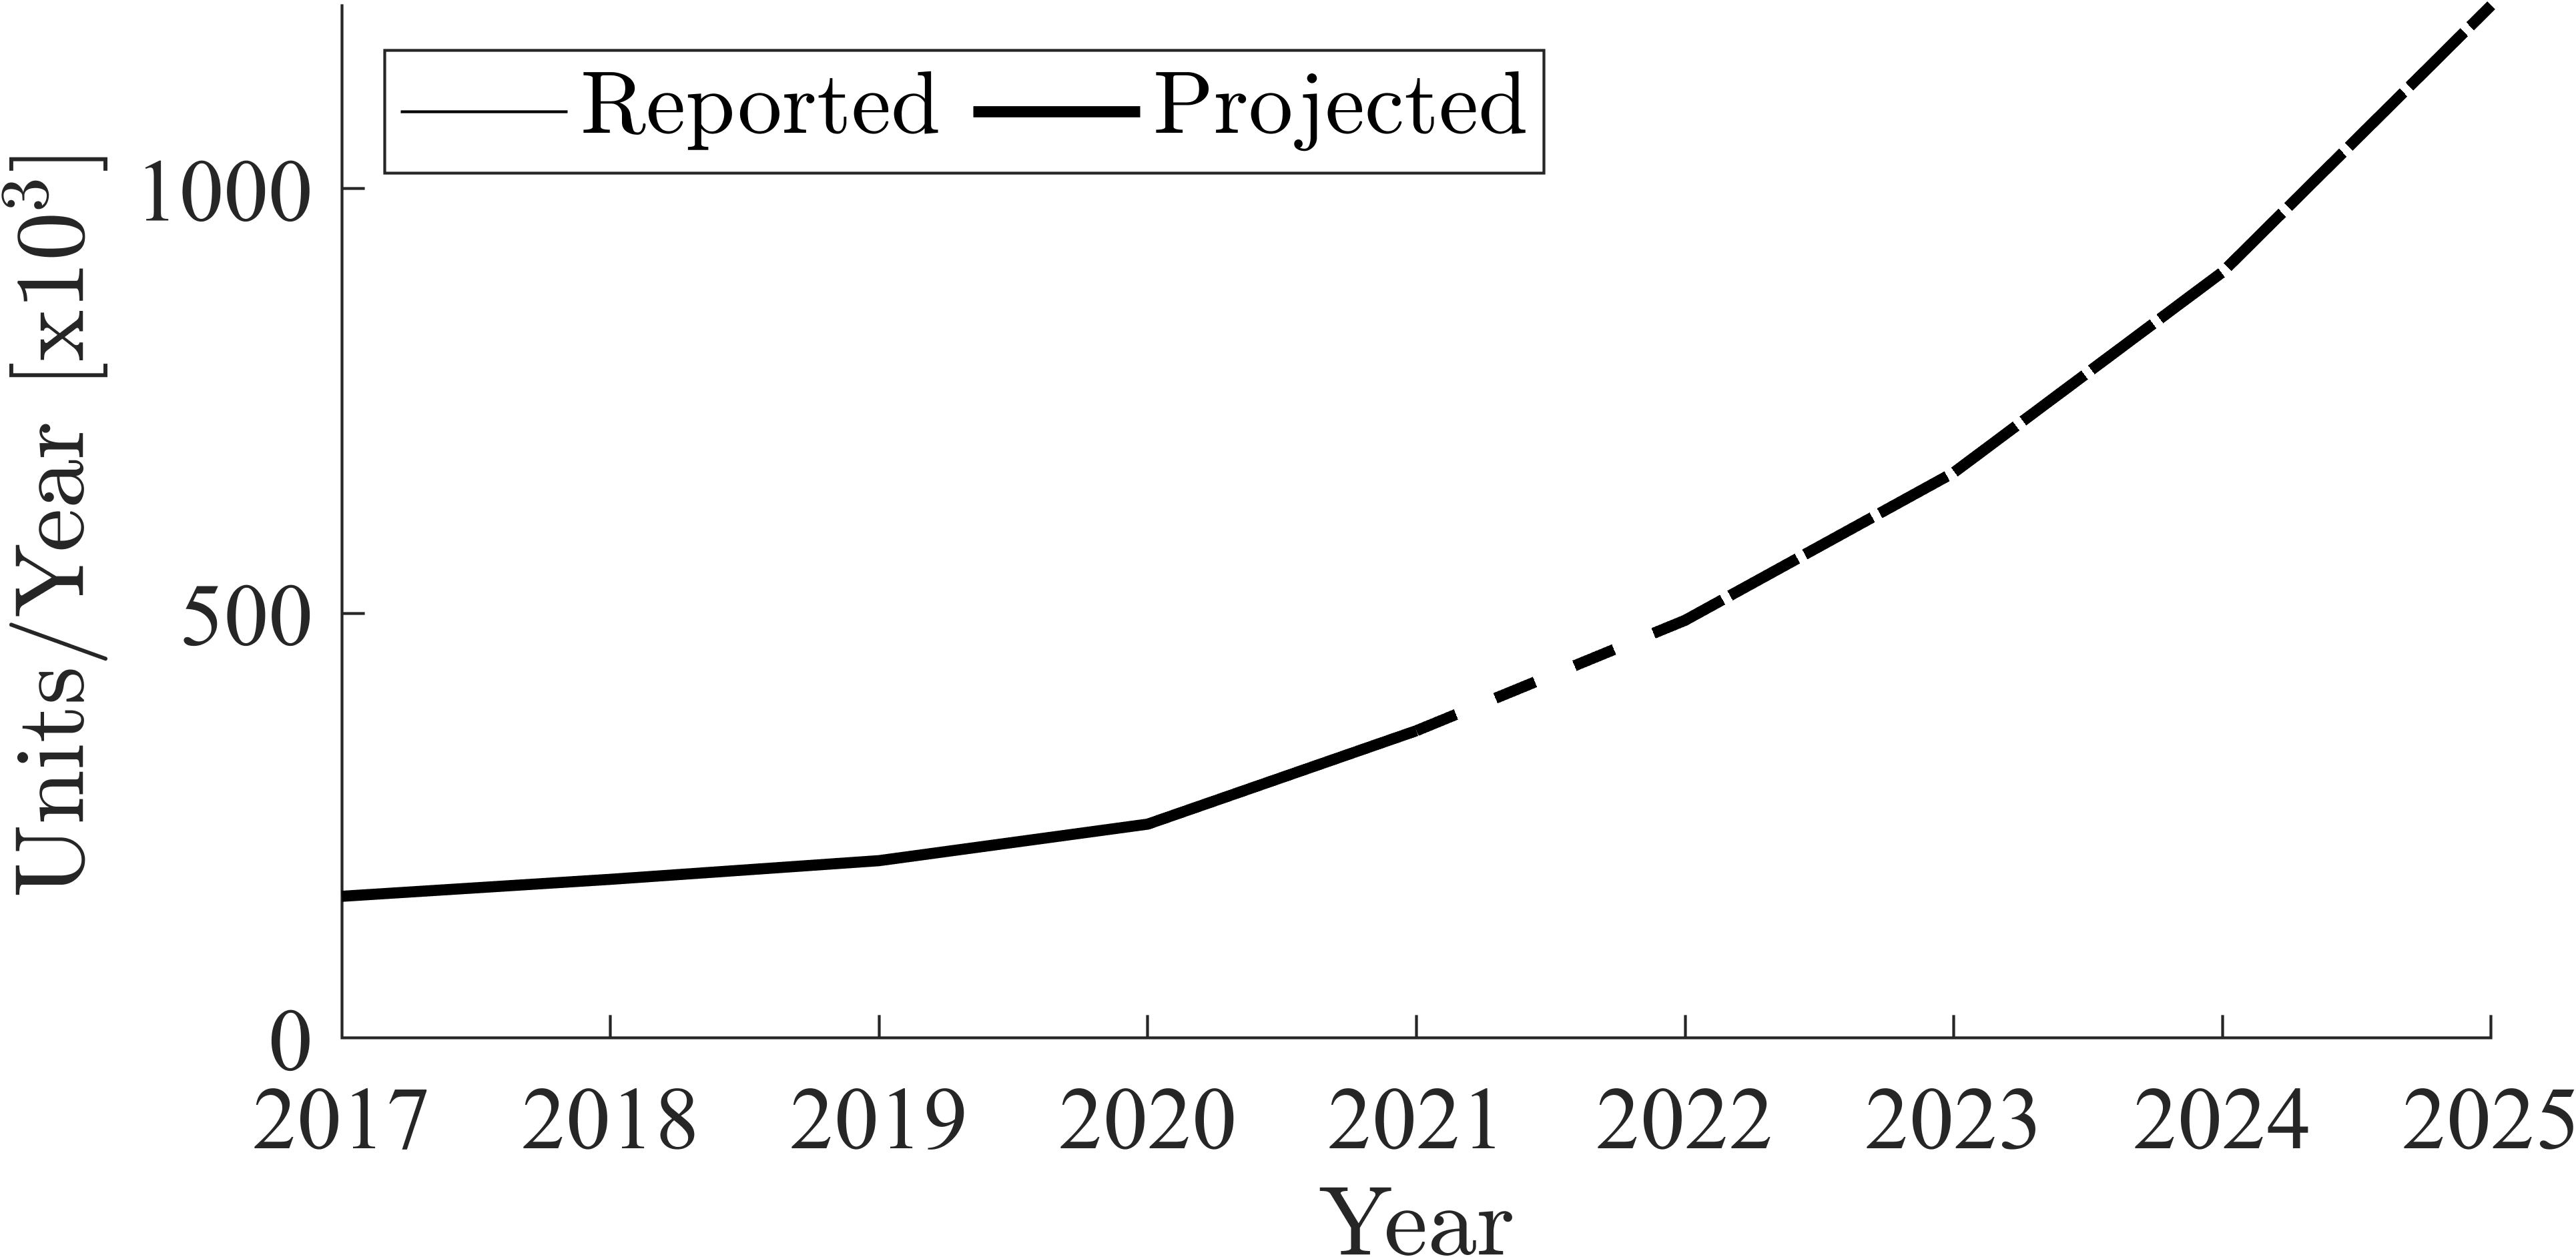
\includegraphics[width= \textwidth]{cb_units_projections.png}
		\label{fig:cobot_stock}
	\end{subfigure}
	\hspace*{\fill}	
	\caption[] {\label{fig:robot_forecasts} Forecasts for robot operational stock. \subref{fig:ir_stock} industrial robots install base forecast and \subref{fig:cobot_stock} cobots install base forecast.}	
\end{figure*}
% ===================================================================================================
%                                                 |                                                 |
%                                                 |                                                 |
% -------------------------------------------- SECTION ---------------------------------------------|
%                                                 |                                                 |
%                                                 |                                                 |
% ===================================================================================================
\newpage
\section{Industrial robot energy consumption support data}\label{sec:app_robot_ener_consumption}
To provide estimates of the worldwide energy consumption of industrial and collaborative robots we surveyed various sources including reports from consulting agencies and non-profit organizations, news articles and manufacturer press releases and data-sheets to determine essential data such as the operational stock and power consumption per type of robot.

\subsection{Industrial robots}
According to \cite{montaqim2015} and available press releases of different robotic companies \cite{fanuc2015, yaskawa2014, ABB2015}, the approximate distribution of the industrial robot install base per manufacturer is shown in Fig.~\ref{fig:manufacturers_pie}.
% ---
\begin{figure*}[!h]
	\centering
	\hspace*{\fill}
	\begin{subfigure}[t]{0.45\textwidth}
		\subcaption{}
		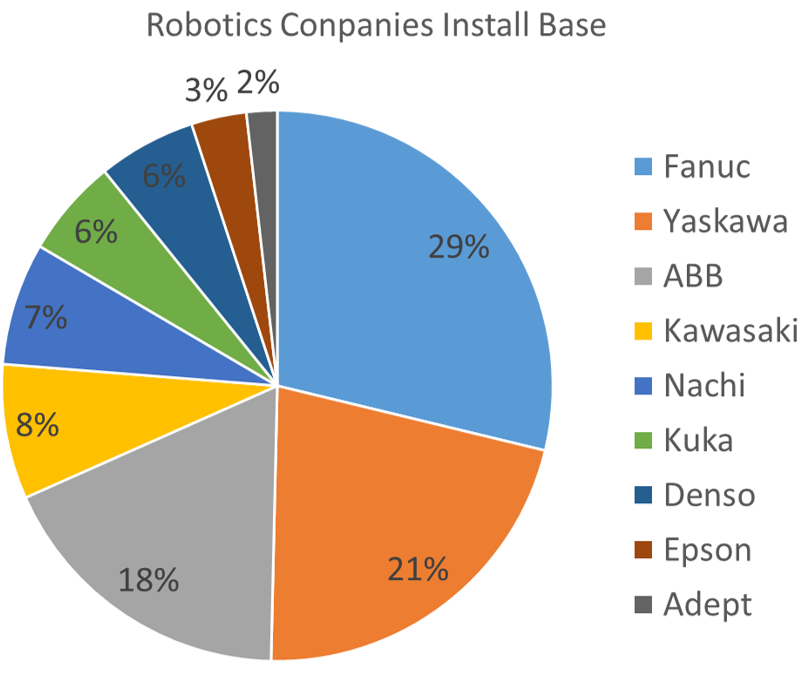
\includegraphics[width= \textwidth]{manufacturers}
		\label{fig:manufacturers_pie}
	\end{subfigure}
	\hfill
	\begin{subfigure}[t]{0.45\textwidth}
		\subcaption{}
		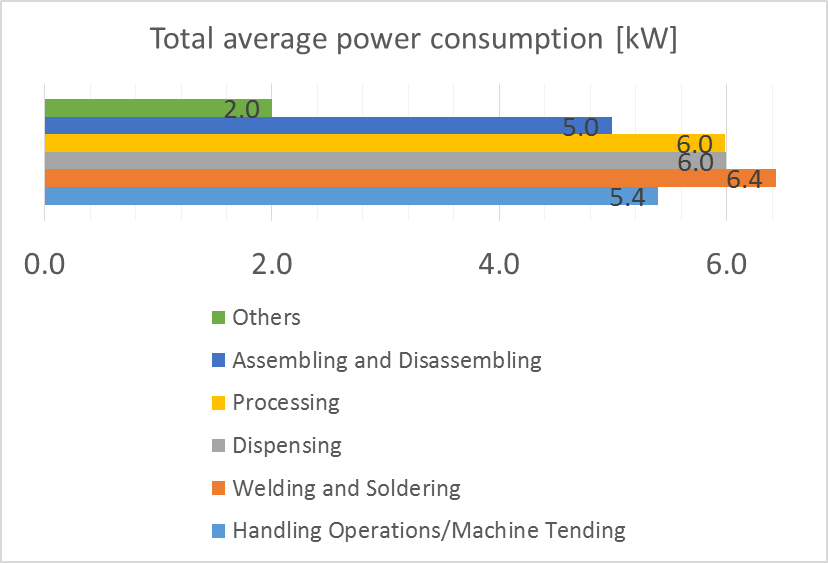
\includegraphics[width=\textwidth]{industrial_robots_average_power_per_category} \label{fig:ir_average_power}
	\end{subfigure}
	\hspace*{\fill}
	\caption[] {\label{fig:ir_statistics} Industrial robots statistics. \subref{fig:manufacturers_pie} Percentage of installed industrial robots per manufacturer and \subref{fig:ir_average_power} average power consumption of industrial robots per category.}
\end{figure*}
% ---

Since Fanuc, Yaskawa, and ABB make for two-thirds of the total install base of industrial robots, we took the power consumption of the robots from those manufacturers to estimate the total power consumption. After surveying the data-sheets for the different robot types in their portfolio, the average power consumption for each model was estimated. Additionally, every manufacturer classifies their robots according to one or more possible applications, which can be grouped into the application categories defined by the IFR. The average power consumption was calculated for every application using the values reported in the robot data-sheets. Finally, the power consumption for each category was computed as a weighted average based on the companies' market share percentage (assuming that 68 \% is the total number of robots)\footnote[1]{These numbers should be used with discretion since there is no available information on which are the most common installed robot models. This information may change the estimation.}. The estimated power consumption per robot application is shown in Fig.~\ref{fig:ir_average_power}. Using these numbers and the estimated operational stock of industrial robots reported in \cite{statista_ir_operational_stock} and by the International Federation of Robotics (see Fig.~\ref{fig:ir_stock}), the estimated worldwide industrial robot energy consumption was computed and shown in Fig.~\ref{fig:ir_energy}.

% ===================================================================================================
\subsection{Collaborative robots}\label{sec:app_cobot_ener_consumption}
%---
\begin{figure}[!h]
	\centering
	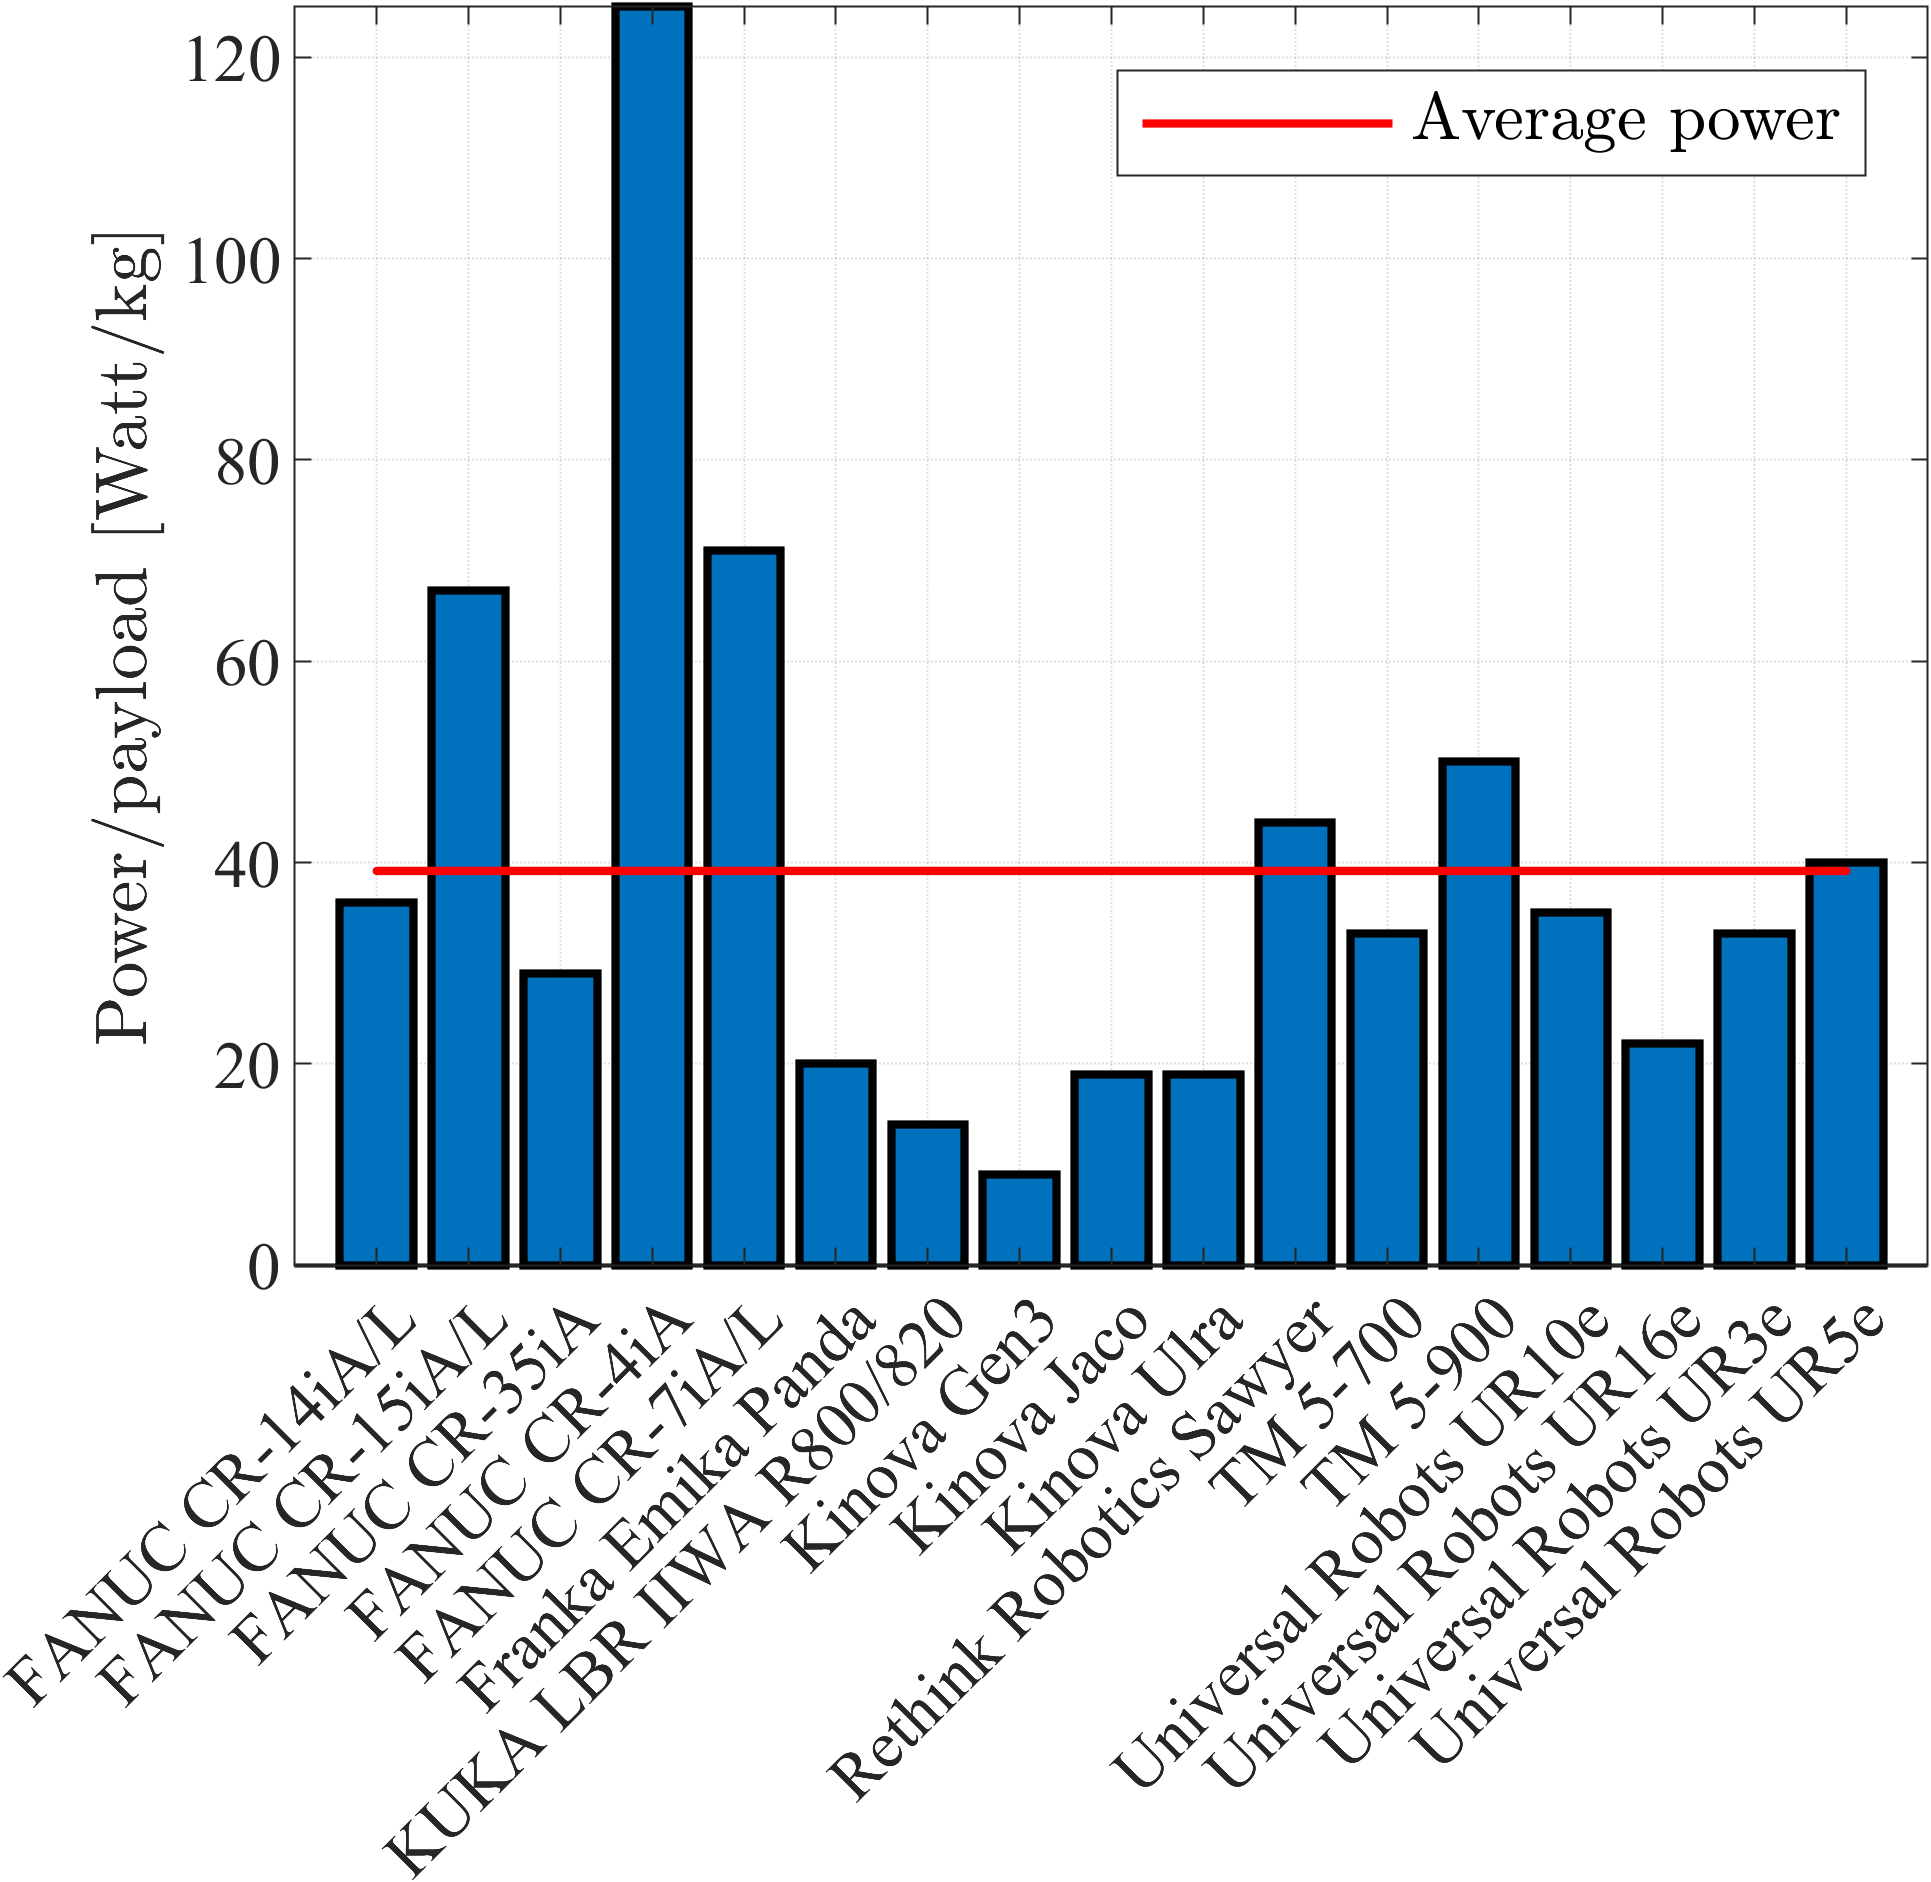
\includegraphics[width=0.45\textwidth]{cobot_watt_per_kg.png}
	\caption{Power consumption per payload for different cobots.}
	\label{fig:cobot_watt_per_kg}
\end{figure}
%---
To approximate the energy consumption of cobots we looked at the power consumption per payload of various manufacturers, see Fig.~\ref{fig:cobot_watt_per_kg} resulting in an average power consumption of approximately 40 W. Together with a typical power consumption of the robot controller of 60 W \cite{Heredia2023BreakingEnergyConsumption}, we consider a total of 100 W power demand. Similar to the industrial robots, the worldwide energy consumption was calculated assuming a 24/7 operation.





\end{document}

%The strength of agent-level intra-cluster skill knowledge integration is quantified by the parameter $\eta$, while $\gamma$ captures the quality of inter-agent knowledge exchange. Additional factors such as $\alpha$ (agent's inherent learning capability), $\beta$ (inter-cluster spread), and $N_r$ (number of agents) influence the overall system dynamics.

% The expression in Fig.\ref{fig:collective_learning_and_skill_manifold_conceptualization}~\textbf{B} formalizes the dynamics of the remaining knowledge about a skill learned by an \ac{eai} agent in a collective, denoted by $\dot{\bar{\sigma}}^{(\mathrm{CL})}_j$, through a set of interpretable components. The governing equation, introduced in Eq.\eqref{eq:collective_knowledge_dynamics}, exhibits dependencies on four main terms. The \emph{agent learning gain} captures the individual agent's ability to acquire knowledge about a skill and is parametrized by $\alpha$. The \emph{intra-cluster knowledge sharing gain} accounts for efficient knowledge propagation between related tasks within the same cluster, modulated by $\eta$. The \emph{inter-cluster similarity gain} reflects the transfer between groups based on structural similarities in the skill manifold, captured by the parameter $\beta$. Finally, the \emph{inter-agent transfer gain} models skill propagation between agents, governed by $\gamma$ and scaled by the number of agents $N_\mathrm{r}$. Together, these components determine whether the remaining knowledge about a skill decays---indicating successful learning---or grows, which signals corruption or forgetting, depending on the interplay of agent-level and collective learning dynamics.

% The expression in Fig.\ref{fig:collective_learning_and_skill_manifold_conceptualization}~\textbf{B}---discussed in detail in Eq.\eqref{eq:collective_knowledge_dynamics} in \nameref{sec:methods}---formalizes the dynamics of the remaining knowledge about a skill $j$ learned by an \ac{eai} agent $i$ in a collective, denoted by $\dot{\bar{\sigma}}^{(\mathrm{CL})}_{i,j}$. This governing equation exhibits dependencies on four main terms that influence the overall dynamics of the system. The \emph{agent learning gain} $\alpha_i$ captures the inherent capacity of the agent $i$ to acquire knowledge about a skill. The \emph{intra-cluster knowledge sharing gain}  $\eta_i$ accounts for the efficient propagation of knowledge to skill $j$ that comes from the skills in the agent's memory belonging to the same cluster. Pairwise \emph{inter-cluster similarity gains}, contained in vector $\bm{\beta}_i$, weigh the transfer of knowledge from other clusters of skills to skill $j$ based on structural similarities in the skill manifold. Furthermore, each pairwise \emph{inter-agent transfer gain} $\gamma$ contained in matrix $\bm{\Gamma}$ models the concurrent propagation of knowledge from the different skills learned by the $N_\mathrm{r}$ agents in the collective. These parameters, together with the number $kappa_{i,k}$ of skills learned from each $k$ cluster that agent $i$ has in memory, determine whether the remaining knowledge about a skill decays, indicating successful learning, or grows, signaling corruption or forgetting, depending on the interplay of agent level and \ac{ cl} dynamics.


% This equation depends on four key terms that govern the behavior of the system:
% % ---
% \begin{itemize}
%     \item \textbf{Agent Learning Gain} ( $\alpha_i$): Represents the inherent ability of agent $i$ to acquire knowledge about skill $j$. The collection of all the agents' gains is contained in the vector $\bm{\alpha}$.
    
%     \item \textbf{Intra-Cluster Knowledge Sharing Gain} ($\eta_i$): Quantifies how efficiently agent $i$ can reinforce skill $j$ through related skills in its memory that belong to the same skill cluster. As before, vector $\bm{\eta}$ gathers the gains for all agents.
    
%     \item \textbf{Inter-Cluster Similarity Matrix} ($\bm{B} \in \mathbb{R}^{N_\mathcal{K}\times N_\mathcal{K}}$): Weighs the contribution of skills from other clusters to skill $j$, based on structural similarity within the skill manifold. For each agent $i$ learning skill $j$, a corresponding vector $\bm{\beta}_{ij}$ is defined from the entries of $\bm{B}$ and the skills in the agent's memory.
    
%     \item \textbf{Inter-Agent Transfer Gains} ($\bm{\Gamma} \in \mathbb{R}^{N_\mathrm{r}\times N_\mathrm{r}} $): The entries $\gamma$ in this matrix model the concurrent transfer of knowledge across the $N_\mathrm{r}$ agents in the collective, through pairwise interactions involving different skills.
% \end{itemize}
% % ---
% Additionally, the number of skills $\kappa_{i,k}$ from each cluster $k$  retained in the $i$-th agent's memory also influences the dynamics. Together, these parameters determine whether the residual knowledge about a skill decreases---indicating successful learning---or increases, which may signal knowledge corruption or forgetting, depending on both agent-level and collective learning dynamics.

% The expression shown in Fig.~\ref{fig:collective_learning_and_skill_manifold_conceptualization}~\textbf{B}---and detailed in Eq.~\eqref{eq:collective_knowledge_dynamics} in \nameref{sec:methods}---describes the dynamics of the remaining knowledge $\dot{\bar{\sigma}}^{(\mathrm{CL})}_{i,j}$ about a skill $j$ learned by an \ac{eai} agent $i$ within a \ac{cl} system. \myhl{This equation depends on four key terms that govern the behavior of the \ac{cl} system: \textbf{Agent Learning Gain} ($\alpha_i$), which represents the inherent ability of agent~$i$ to acquire knowledge about skill~$j$, with the collection of all agents' gains contained in the vector~$\bm{\alpha}$; \textbf{Intra-Cluster Knowledge Sharing Gain} ($\eta_i$), which quantifies how efficiently agent~$i$ can reinforce skill~$j$ through related skills in its memory that belong to the same skill cluster, with vector~$\bm{\eta}$ gathering the gains for all agents; \myhl{\textbf{Inter-Cluster Similarity Matrix} ($\bm{B} \in \mathbb{R}^{N_\mathcal{K} \times N_\mathcal{K}}$), which weighs the contribution of skills from other clusters to skill~$j$ based on structural similarity within the skill manifold---for each agent~$i$ learning skill~$j$, a corresponding vector~$\bm{\beta}{ij}$ is defined from the entries of~$\bm{B}$ and the skills in the agent's memory}; and \textbf{Inter-Agent Transfer Gains} ($\bm{\Gamma} \in \mathbb{R}^{N\mathrm{r} \times N_\mathrm{r}}$), where the entries~$\gamma$ model the concurrent transfer of knowledge across the~$N_\mathrm{r}$ agents in the collective, through pairwise interactions involving different skills. Additionally, the number of skills~$\kappa_{i,k}$ from each cluster~$k$ retained in the $i$-th agent's memory also influences the dynamics. Together, these parameters determine whether the residual knowledge about a skill decreases---indicating successful learning---or increases, which may signal knowledge corruption or forgetting, depending on both agent-level and collective learning dynamics.}